% =====================================================================================
%  score: Sockets, Columns and Tail Risk -- a dark-mode deep-dive tutorial
%  Build:  xelatex main.tex (x3)   -- see README.txt in this folder
%  Fonts:  Carlito (text), DejaVu Sans Mono (code), Latin Modern Math (math)
% =====================================================================================
\documentclass[11pt,oneside]{report}
\usepackage[letterpaper,margin=0.8in,top=0.8in,bottom=0.85in,headheight=14pt]{geometry}
\usepackage{amsmath,amssymb,amsthm,mathtools}
\usepackage{fontspec}
\usepackage{unicode-math}
\setmainfont{Carlito}[Extension=.ttf,UprightFont=*-Regular,BoldFont=*-Bold,ItalicFont=*-Italic,BoldItalicFont=*-BoldItalic,Ligatures=TeX]
\setsansfont{Carlito}[Extension=.ttf,UprightFont=*-Regular,BoldFont=*-Bold,ItalicFont=*-Italic,BoldItalicFont=*-BoldItalic,Ligatures=TeX]
\setmonofont{DejaVu Sans Mono}[Scale=0.84,HyphenChar=None]
\setmathfont{latinmodern-math.otf}
\usepackage{xcolor}
\usepackage{graphicx}
\usepackage{needspace}
\usepackage{tabularx,booktabs,array,multirow,longtable}
\usepackage[shortlabels]{enumitem}
\usepackage{fancyhdr}
\usepackage{titlesec}
\usepackage{float}
\usepackage[font=small,labelfont={bf,color=acc},textfont={color=muted}]{caption}
\usepackage{tikz}
\usetikzlibrary{arrows.meta,positioning,calc,decorations.pathreplacing,fit,backgrounds,shapes.geometric}
\usepackage{pgfplots}
\pgfplotsset{compat=1.18}
\usepackage[most]{tcolorbox}
\usepackage{listings}
\usepackage[hidelinks=false,colorlinks=true,linkcolor=acc,citecolor=grn,urlcolor=strc,
            pdftitle={score: Sockets, Columns and Tail Risk -- A Deep-Dive Tutorial},
            pdfauthor={score project}]{hyperref}
\usepackage[nameinlink]{cleveref}
\usepackage{xurl}

% ------------------------------------------------------------ palette (dark mode)
\definecolor{bg}{HTML}{0D1117}
\definecolor{fg}{HTML}{E6EDF3}
\definecolor{muted}{HTML}{9DA7B3}
\definecolor{acc}{HTML}{58A6FF}
\definecolor{grn}{HTML}{3FB950}
\definecolor{yel}{HTML}{E3B341}
\definecolor{red}{HTML}{FF7B72}
\definecolor{pur}{HTML}{D2A8FF}
\definecolor{org}{HTML}{FFA657}
\definecolor{codebg}{HTML}{161B22}
\definecolor{panel}{HTML}{11161D}
\definecolor{codeframe}{HTML}{3D444D}
\definecolor{strc}{HTML}{A5D6FF}

\makeatletter
\AtBeginDocument{\pagecolor{bg}\color{fg}\def\normalcolor{\color{fg}}}
\makeatother
\tcbset{colupper=fg,collower=fg}
\setlength{\parindent}{0pt}
\setlength{\parskip}{5pt plus 1pt}
\setlist{itemsep=2pt,topsep=3pt,leftmargin=1.4em}
\setlist[itemize]{label=\textcolor{acc}{\textbullet}}
\renewcommand{\arraystretch}{1.18}
\linespread{1.04}
\setlength{\emergencystretch}{3em}

% ------------------------------------------------------------ headings
\titleformat{\chapter}[display]
  {\normalfont\color{fg}}
  {\large\color{muted}\MakeUppercase{\chaptertitlename}\ \thechapter}
  {4pt}
  {\Huge\bfseries\color{acc}\raggedright}
  [\vspace{4pt}{\color{codeframe}\titlerule[0.8pt]}]
\titlespacing*{\chapter}{0pt}{-10pt}{18pt}
\titleformat{\section}{\Large\bfseries\color{acc}}{\thesection}{0.7em}{}
\titleformat{\subsection}{\large\bfseries\color{strc}}{\thesubsection}{0.6em}{}
\titleformat{\subsubsection}[runin]{\normalsize\bfseries\color{yel}}{}{0pt}{}[.]
\titlespacing*{\section}{0pt}{14pt}{6pt}
\titlespacing*{\subsection}{0pt}{11pt}{4pt}
\setcounter{secnumdepth}{2}
\setcounter{tocdepth}{1}

\pagestyle{fancy}
\fancyhf{}
\renewcommand{\headrulewidth}{0pt}
\fancyhead[L]{\small\color{muted}\leftmark}
\fancyhead[R]{\small\color{muted}score deep dive}
\fancyfoot[C]{\small\color{muted}\thepage}
\renewcommand{\chaptermark}[1]{\markboth{\thechapter.\ #1}{}}
\fancypagestyle{plain}{\fancyhf{}\fancyfoot[C]{\small\color{muted}\thepage}}

% ------------------------------------------------------------ theorem-like environments
\theoremstyle{definition}
\newtheorem{theorem}{Theorem}[chapter]
\newtheorem{definition}[theorem]{Definition}
\newtheorem{lemma}[theorem]{Lemma}
\newtheorem{proposition}[theorem]{Proposition}
\newtheorem{corollary}[theorem]{Corollary}
\newtheorem{example}[theorem]{Worked example}
\newtheorem{claim}[theorem]{Claim}
\crefname{example}{worked example}{worked examples}
\crefname{definition}{definition}{definitions}
\crefname{lemma}{lemma}{lemmas}
\crefname{proposition}{proposition}{propositions}
\crefname{corollary}{corollary}{corollaries}
\crefname{claim}{claim}{claims}
\crefname{exercise}{exercise}{exercises}
\tcolorboxenvironment{theorem}{enhanced,breakable,colback=codebg,colframe=acc,boxrule=0.7pt,arc=2pt,left=7pt,right=7pt,top=5pt,bottom=5pt,before skip=8pt,after skip=8pt}
\tcolorboxenvironment{lemma}{enhanced,breakable,colback=codebg,colframe=acc,boxrule=0.7pt,arc=2pt,left=7pt,right=7pt,top=5pt,bottom=5pt,before skip=8pt,after skip=8pt}
\tcolorboxenvironment{proposition}{enhanced,breakable,colback=codebg,colframe=acc,boxrule=0.7pt,arc=2pt,left=7pt,right=7pt,top=5pt,bottom=5pt,before skip=8pt,after skip=8pt}
\tcolorboxenvironment{corollary}{enhanced,breakable,colback=codebg,colframe=acc,boxrule=0.7pt,arc=2pt,left=7pt,right=7pt,top=5pt,bottom=5pt,before skip=8pt,after skip=8pt}
\tcolorboxenvironment{claim}{enhanced,breakable,colback=codebg,colframe=acc,boxrule=0.7pt,arc=2pt,left=7pt,right=7pt,top=5pt,bottom=5pt,before skip=8pt,after skip=8pt}
\tcolorboxenvironment{definition}{enhanced,breakable,colback=codebg,colframe=grn,boxrule=0.7pt,arc=2pt,left=7pt,right=7pt,top=5pt,bottom=5pt,before skip=8pt,after skip=8pt}
\tcolorboxenvironment{example}{enhanced,breakable,colback=panel,colframe=org,boxrule=0.7pt,arc=2pt,left=7pt,right=7pt,top=5pt,bottom=5pt,before skip=8pt,after skip=8pt}
\renewcommand{\qedsymbol}{\textcolor{acc}{$\blacksquare$}}
\makeatletter
\renewenvironment{proof}[1][\proofname]{\par\pushQED{\qed}\normalfont\topsep6\p@\@plus6\p@\relax
  \trivlist\item[\hskip\labelsep\color{acc}\bfseries\itshape #1.]\ignorespaces}{\popQED\endtrivlist\@endpefalse}
\makeatother

% ------------------------------------------------------------ pedagogical boxes
\newtcolorbox{layman}[1][]{enhanced,breakable,colback=panel,colframe=yel,boxrule=0.6pt,arc=2pt,
  left=7pt,right=7pt,top=4pt,bottom=4pt,fonttitle=\bfseries,colbacktitle=codeframe,coltitle=yel,
  title={Plain-language analogy},#1}
\newtcolorbox{remarkbox}[1][]{enhanced,breakable,colback=panel,colframe=pur,boxrule=0.6pt,arc=2pt,
  left=7pt,right=7pt,top=4pt,bottom=4pt,fonttitle=\bfseries,colbacktitle=codeframe,coltitle=pur,
  title={Remark},#1}
\newtcolorbox{history}[1][]{enhanced,breakable,colback=panel,colframe=org,boxrule=0.6pt,arc=2pt,
  left=7pt,right=7pt,top=4pt,bottom=4pt,fonttitle=\bfseries,colbacktitle=codeframe,coltitle=org,
  title={Historical note},#1}
\newtcolorbox{pitfall}[1][]{enhanced,breakable,colback=panel,colframe=red,boxrule=0.6pt,arc=2pt,
  left=7pt,right=7pt,top=4pt,bottom=4pt,fonttitle=\bfseries,colbacktitle=codeframe,coltitle=red,
  title={Pitfall},#1}
\newtcolorbox{objectives}[1][]{enhanced,breakable,colback=codebg,colframe=acc,boxrule=0.6pt,arc=2pt,
  left=7pt,right=7pt,top=4pt,bottom=4pt,fonttitle=\bfseries,colbacktitle=codeframe,coltitle=acc,
  title={Learning objectives},#1}
\newtcolorbox{verified}[1][]{enhanced,breakable,colback=codebg,colframe=grn,boxrule=0.6pt,arc=2pt,
  left=7pt,right=7pt,top=4pt,bottom=4pt,fonttitle=\bfseries,colbacktitle=codeframe,coltitle=grn,
  title={Verified by running code},#1}

% exercises: numbered per chapter, hints live in Appendix A
\newcounter{exercise}[chapter]
\renewcommand{\theexercise}{\thechapter.\arabic{exercise}}
\newenvironment{exercises}{\Needspace{6\baselineskip}\begin{tcolorbox}[enhanced,breakable,colback=codebg,colframe=grn,boxrule=0.7pt,arc=2pt,
  left=7pt,right=7pt,top=5pt,bottom=5pt,fonttitle=\bfseries\large,colbacktitle=codeframe,coltitle=grn,
  title={Engineering questions and exercises}]
  \small\color{muted}Difficulty: \textcolor{grn}{$\bullet$} warm-up \quad \textcolor{yel}{$\bullet\bullet$} design/derive \quad \textcolor{red}{$\bullet\bullet\bullet$} research-grade.
  Hints (not solutions) are in \cref{app:hints}.\color{fg}\par\vspace{2pt}\setlength{\parskip}{3pt}}{\end{tcolorbox}}
\newcommand{\ex}[2]{\par\refstepcounter{exercise}\label{#1}\textbf{\color{grn}Exercise \theexercise}\ #2\ }
\newcommand{\lvA}{\textcolor{grn}{$\bullet$}}
\newcommand{\lvB}{\textcolor{yel}{$\bullet\bullet$}}
\newcommand{\lvC}{\textcolor{red}{$\bullet\bullet\bullet$}}
\newcommand{\hint}[2]{\par\textbf{\color{grn}\ref{#1}.}\ #2}

% ------------------------------------------------------------ inline helpers
\newcommand{\cc}[1]{\leavevmode{\ttfamily\color{org}\detokenize{#1}}}
\newcommand{\file}[1]{\leavevmode{\ttfamily\color{strc}\detokenize{#1}}}
\newcommand{\VaR}{\mathrm{VaR}}
\newcommand{\ES}{\mathrm{ES}}
\newcommand{\CVaR}{\mathrm{CVaR}}
\newcommand{\fl}{\mathrm{fl}}
\newcommand{\ulp}{\mathrm{ulp}}
\newcommand{\R}{\mathbb{R}}
\newcommand{\N}{\mathbb{N}}
\newcommand{\Prob}{\mathbb{P}}
\newcommand{\E}{\mathbb{E}}
\newcommand{\ord}[1]{X_{(#1)}}
\newcommand{\hex}[1]{\text{\ttfamily\color{org}#1}}

% ------------------------------------------------------------ code listings
\lstdefinestyle{dark}{
  basicstyle=\ttfamily\fontsize{8.4}{10.4}\selectfont\color{fg},
  keywordstyle=\color{red},
  keywordstyle=[2]\color{pur},
  keywordstyle=[3]\color{acc},
  commentstyle=\color{muted}\itshape,
  stringstyle=\color{strc},
  numbers=left, numberstyle=\fontsize{7}{9}\selectfont\color{codeframe!60!muted}, numbersep=7pt,
  showstringspaces=false, columns=fullflexible, keepspaces=true,
  breaklines=true, breakatwhitespace=false, tabsize=4, upquote=true,
  postbreak=\mbox{\textcolor{muted}{$\hookrightarrow$}\space},
  literate={—}{{\textemdash}}1 {–}{{\textendash}}1 {→}{{$\rightarrow$}}1 {≥}{{$\geq$}}1,
}
\lstdefinestyle{cppdark}{style=dark,language=C++,
  morekeywords={nullptr,constexpr,noexcept,override,final,static_cast,using,namespace,throw,explicit,virtual,default,delete},
  morekeywords=[2]{size_t,uint8_t,uint16_t,uint32_t,int64_t,std,string,vector,optional,function,unique_ptr,Frame,FrameCodec,JsonFrameCodec,EventLoop,Connection,Server,Bar,ColumnStore,ColumnStoreV1,IngestionSource,SocketHandle,IoEvent,IoCallback,CodecFactory,RiskStats,HistoricalTail,DomainError,EmptySeriesError,NotImplementedError,ScoreException,DimensionMismatchError,json},
  morekeywords=[3]{historical_var,historical_cvar,historical_tail,log_returns,encode,feed,try_decode,register_io,unregister,run,stop,listen,send,close,append,scan,symbols,count,ingest,name,sort,accumulate,max},
}
\lstdefinestyle{pydark}{style=dark,language=Python,
  morekeywords=[2]{np,math,date,timedelta,dataclass,TickerConfig,MarketData,cached_property},
  morekeywords=[3]{standard_normal,cumsum,exp,normal,history,iloc,concatenate},
}
\lstdefinestyle{plaindark}{style=dark,language={},numbers=none}
\lstset{style=cppdark}
\newtcblisting[auto counter,number within=chapter,crefname={listing}{listings}]{code}[3][]{listing only,breakable,enhanced,
  listing options={style=cppdark},colback=codebg,colframe=codeframe,boxrule=0.5pt,arc=2pt,left=16pt,right=4pt,top=1pt,bottom=1pt,boxsep=2pt,
  title={\small Listing~\thetcbcounter\quad\ttfamily #2\hfill\rmfamily\itshape illustrative sketch, tested},fonttitle=\color{muted},colbacktitle=panel,coltitle=muted,toptitle=1pt,bottomtitle=1pt,label={#3},#1}
\newtcblisting[use counter from=code,crefname={listing}{listings}]{pycode}[3][]{listing only,breakable,enhanced,
  listing options={style=pydark},colback=codebg,colframe=codeframe,boxrule=0.5pt,arc=2pt,left=16pt,right=4pt,top=1pt,bottom=1pt,boxsep=2pt,
  title={\small Listing~\thetcbcounter\quad\ttfamily #2},fonttitle=\color{muted},colbacktitle=panel,coltitle=muted,toptitle=1pt,bottomtitle=1pt,label={#3},#1}
\newtcblisting[use counter from=code,crefname={listing}{listings}]{progout}[3][]{listing only,breakable,enhanced,
  listing options={style=plaindark,basicstyle=\ttfamily\fontsize{8.2}{10.2}\selectfont\color{grn}},colback=black!60!bg,colframe=grn!50!codeframe,boxrule=0.5pt,arc=2pt,left=6pt,right=4pt,top=1pt,bottom=1pt,boxsep=2pt,
  title={\small Listing~\thetcbcounter\quad program output: #2},fonttitle=\color{muted},colbacktitle=panel,coltitle=muted,toptitle=1pt,bottomtitle=1pt,label={#3},#1}
% verbatim excerpt of a repository file: \repo[lst opts]{path}{caption}{label}
\newtcolorbox[use counter from=code,crefname={listing}{listings}]{repobox}[2]{enhanced,breakable,colback=codebg,colframe=codeframe,boxrule=0.5pt,arc=2pt,
  left=16pt,right=4pt,top=1pt,bottom=2pt,boxsep=2pt,
  title={\small\color{muted}Listing~\thetcbcounter\quad\ttfamily\color{strc}\detokenize{#1}\hfill\color{muted}\rmfamily\itshape verbatim from repository},
  colbacktitle=panel,toptitle=1pt,bottomtitle=1pt,label={#2},lowerbox=visible,segmentation style={draw=codeframe,dashed}}
\newcommand{\repo}[4][]{\begin{repobox}{#2}{#4}\lstinputlisting[style=cppdark,#1]{repo/#2}\tcblower\small\color{muted}#3\end{repobox}}
\newcommand{\repopy}[4][]{\begin{repobox}{#2}{#4}\lstinputlisting[style=pydark,#1]{repo/#2}\tcblower\small\color{muted}#3\end{repobox}}
\newcommand{\repomd}[4][]{\begin{repobox}{#2}{#4}\lstinputlisting[style=plaindark,#1]{repo/#2}\tcblower\small\color{muted}#3\end{repobox}}
\tcbset{lowerbox=visible,segmentation style={draw=codeframe,dashed}}

% ------------------------------------------------------------ pgfplots / tikz dark styling
\pgfplotsset{
  darkaxis/.style={
    axis line style={muted}, tick style={muted}, every tick label/.append style={font=\footnotesize,color=muted},
    label style={font=\small,color=fg}, title style={color=fg},
    grid style={codeframe,line width=0.3pt}, major grid style={codeframe},
    legend style={fill=codebg,draw=codeframe,text=fg,font=\footnotesize},
    tick label style={/pgf/number format/fixed}, scaled ticks=false,
  }
}
\tikzset{
  byte/.style={draw=muted,minimum width=8.2mm,minimum height=6.5mm,inner sep=0pt,font=\ttfamily\footnotesize,text=fg},
  boxn/.style={draw=acc,rounded corners=2pt,fill=codebg,text=fg,inner sep=4pt,font=\small,align=center},
  arr/.style={-{Stealth[length=2mm]},thick,draw=muted},
  lbl/.style={font=\footnotesize,text=muted},
}

\begin{document}
% ---------------------------------------------------------------- title page
\begin{titlepage}
\pagecolor{bg}\color{fg}
\vspace*{0.6in}
{\color{muted}\large A deep-dive tutorial on the \texttt{score} repository}\par
\vspace{10pt}
{\fontsize{38}{44}\selectfont\bfseries\color{acc} Sockets, Columns\\[2pt] and Tail Risk}\par
\vspace{14pt}
{\Large\color{fg} Designing a networked stock-risk engine from first principles:\\ TCP framing, reactors, columnar storage, Value at Risk,\\ and the floating-point bug that hid in a confidence level}\par
\vspace{26pt}
{\color{codeframe}\rule{\linewidth}{0.8pt}}\par
\vspace{12pt}
\begin{tikzpicture}
  % a small decorative frame header: 4 length bytes then payload
  \foreach \i/\b in {0/00,1/00,2/00,3/28}{\node[byte,draw=yel,text=yel] at (\i*0.86,0) {\b};}
  \foreach \i/\b in {4/7B,5/22,6/63,7/6F,8/6E,9/66,10/22,11/3A,12/30,13/2E,14/39,15/35}{\node[byte,draw=acc] at (\i*0.86,0) {\b};}
  \node[byte,draw=muted,text=muted] at (16*0.86,0) {\dots};
  \draw[decorate,decoration={brace,amplitude=5pt,mirror},draw=yel] (-0.4,-0.45) -- (3*0.86+0.4,-0.45) node[midway,below=6pt,font=\footnotesize,text=yel]{length = 40 (big-endian)};
  \draw[decorate,decoration={brace,amplitude=5pt,mirror},draw=acc] (4*0.86-0.4,-0.45) -- (15*0.86+0.4,-0.45) node[midway,below=6pt,font=\footnotesize,text=acc]{\texttt{\{"conf":0.95,...} (JSON payload)};
\end{tikzpicture}
\vspace{22pt}

\begin{minipage}[t]{0.55\linewidth}
\color{muted}\small
\textbf{\color{fg}What this is.} A textbook-style companion to the \texttt{score} C++23 library's
storage, networking and risk extensions. Every number, byte and bit pattern in it was produced by
running code; every repository listing is quoted verbatim from the working tree.\par
\vspace{6pt}
\textbf{\color{fg}How to read it.} Work each chapter in order: objectives, exposition, worked examples,
then the engineering questions. Hints, not solutions, are in \cref{app:hints}.
\end{minipage}\hfill
\begin{minipage}[t]{0.38\linewidth}
\color{muted}\small
\textbf{\color{fg}Repository state.} Branch \texttt{formatter}; newest changelog entry dated 2026-10-17.\par
\vspace{6pt}
\textbf{\color{fg}Measurements.} Benchmarks ran on an Apple M3 Max (14 cores), macOS 26.6.2, Apple clang 21.\par
\vspace{6pt}
\textbf{\color{fg}Compiled.} \today.
\end{minipage}
\vfill
{\color{muted}\footnotesize Prepared with AI assistance (Claude). The text and figures are largely AI-generated and were checked by
re-running the code that produced every quoted number; please review before relying on it.}
\end{titlepage}

% ---------------------------------------------------------------- abstract
\chapter*{Abstract}
\addcontentsline{toc}{chapter}{Abstract}
\markboth{Abstract}{}
The \texttt{score} repository began as a C++23 library of descriptive statistics and stock metrics
(log-returns, the Sharpe ratio, maximum drawdown) exposed to Python through nanobind. It had three
conspicuous gaps: nothing was ever \emph{stored} (prices arrived either from live \texttt{yfinance}
calls or from a synthetic geometric-Brownian-motion generator, and both were discarded after use);
nothing measured \emph{tail} risk (no Value at Risk, no Expected Shortfall); and there was no
\emph{networking or concurrency} code at all. A structured design interview, a ``grilling session'',
turned the vague wish ``add a database and some networking'' into twelve falsifiable decisions and a
twelve-phase roadmap.

This tutorial teaches the ideas behind those decisions from first principles. We treat TCP as what
it is, an ordered byte stream with no message boundaries, and prove that a length-prefixed decoder
reconstructs messages under every possible segmentation. We compare thread-per-connection,
\texttt{poll}, \texttt{epoll}/\texttt{kqueue} and \texttt{io\_uring} with a cost model and with
measurements taken on the author's machine. We derive the byte-level advantage of columnar storage
for the one query a risk engine runs constantly. We define Value at Risk and Expected Shortfall
precisely, relate the repository's estimator to order statistics and to the Hyndman--Fan quantile
taxonomy, and verify a counterexample to the subadditivity of VaR. Finally, we dissect a real
IEEE-754 defect found while implementing VaR, in which \(1.0-0.90\) evaluates to
\(0.09999999999999998\), bound the conditions under which the repository's \(10^{-9}\) guard is
provably correct, and set it beside three historical numerical failures.

Each chapter ends with engineering questions specific to this codebase. Citations point to primary
sources: original papers, standards, and official reports.

\begin{remarkbox}[title={Colour conventions used in every figure}]
\textcolor{acc}{Blue}: interfaces, structure, the ``current'' item.
\textcolor{grn}{Green}: implemented, correct, done.
\textcolor{yel}{Yellow}: length prefixes, headers, ``next''.
\textcolor{red}{Red}: failure, loss, the thing that breaks.
\textcolor{pur}{Purple}: Python producers and remarks.
\textcolor{org}{Orange}: worked examples, inline code, historical notes.
\end{remarkbox}

% ---------------------------------------------------------------- contents
{\hypersetup{linkcolor=fg}\setlength{\parskip}{0pt}\tableofcontents}

% ---------------------------------------------------------------- notation
\chapter*{Notation and glossary}
\addcontentsline{toc}{chapter}{Notation and glossary}
\markboth{Notation and glossary}{}
\begin{center}
\small
\begin{tabularx}{\linewidth}{@{}>{\leavevmode\color{yel}}l X@{}}
\toprule
\textcolor{muted}{Symbol} & \textcolor{muted}{Meaning}\\
\midrule
$P_t$ & closing price on trading day $t$\\
$r_t=\ln(P_t/P_{t-1})$ & daily log-return (\cc{risk::log_returns})\\
$X$, $L=-X$ & return (profit-and-loss fraction) and the corresponding loss\\
$F_X(x)=\Prob(X\le x)$ & cumulative distribution function (CDF) of $X$\\
$F_n$ & empirical CDF of a sample of size $n$: $F_n(x)=\frac1n\#\{i:X_i\le x\}$\\
$\ord{1}\le\dots\le\ord{n}$ & order statistics (the sample sorted ascending, as \cc{std::sort} leaves it)\\
$c$, $\alpha$ & confidence level, e.g.\ $0.95$ (the code's \cc{confidence_level})\\
$p=1-c$ & tail probability\\
$k=\lfloor pn+\varepsilon\rfloor$ & the code's \cc{tail_index}, $\varepsilon=10^{-9}$\\
$\VaR_c$, $\ES_c$ & Value at Risk and Expected Shortfall (CVaR) at confidence $c$\\
$\fl(x)$ & the IEEE-754 binary64 number nearest to the real $x$ (round-to-nearest-even)\\
$u=2^{-53}$ & unit roundoff of binary64\\
$\ulp(x)$ & unit in the last place: spacing of binary64 numbers near $x$\\
$n$ & number of connections (\cref{ch:conc}) or of observations (\cref{ch:risk,ch:float}); context decides\\
$\Theta$, $O$ & asymptotic tight bound and upper bound\\
\bottomrule
\end{tabularx}
\end{center}

\begin{center}
\small
\begin{tabularx}{\linewidth}{@{}>{\leavevmode\bfseries\color{acc}}p{3.2cm} X@{}}
\toprule
\textcolor{muted}{Term} & \textcolor{muted}{Definition}\\
\midrule
Byte stream & An ordered, reliable sequence of bytes with no record boundaries (TCP's service model).\\
Frame & One application message plus the framing bytes that delimit it on the wire.\\
Codec & Encoder/decoder pair turning frames into bytes and back (\cc{FrameCodec}).\\
Reactor & Event-demultiplexing pattern: the loop learns a handle is \emph{ready}, then calls the handler, which performs the I/O.\\
Proactor & The loop \emph{starts} I/O on the handler's behalf and calls it on \emph{completion}.\\
Readiness API & \cc{select}, \cc{poll}, \cc{epoll}, \cc{kqueue}: report which descriptors can make progress.\\
Completion API & \cc{io_uring} (Linux), IOCP (Windows): report which submitted operations finished.\\
Column store & Storage that keeps each attribute's values contiguous rather than each record's.\\
OHLCV & Open, high, low, close, volume: one daily bar (\cc{score::db::Bar}).\\
Historical simulation & Estimating risk from the empirical distribution of past returns, without a parametric model.\\
Coherent risk measure & A risk measure satisfying the four axioms of Artzner et al.\ (\cref{def:coherent}).\\
Scaffolding & An interface plus stub bodies that throw \cc{score::NotImplementedError}.\\
\bottomrule
\end{tabularx}
\end{center}



\chapter{Design Method: From a Vague Idea to Twelve Falsifiable Decisions}\label{ch:design}

\begin{objectives}
After this chapter you should be able to:
\begin{itemize}
\item describe the state of \texttt{score} before the extension, and name its three structural gaps;
\item explain what makes a design decision \emph{falsifiable}, and write a falsifier for each of the twelve decisions;
\item explain the ``decision frontier'' technique a grilling session uses to order questions;
\item argue, with a counting argument, why the extension was built as interfaces first;
\item justify scaffolding with stubs that \emph{throw} rather than stubs that return defaults.
\end{itemize}
{\small\color{muted}\textbf{Chapter references:} Parnas~\cite{parnas1972criteria}; Martin~\cite{martin2003agile}; Gamma et al.~\cite{gamma1994design};
Brooks~\cite{brooks1975mythical}.}
\end{objectives}

\section{Where the repository started}\label{sec:start}
\texttt{score} is a C++23 shared library, \texttt{libscore\_core}, with a C API and nanobind bindings to a Python
package. Before this work it computed descriptive statistics, log-returns, a Sharpe ratio and maximum drawdown
(\cref{fig:arch}). It had three structural gaps, and every later chapter grows out of one of them.

\begin{enumerate}[label=\textbf{\color{yel}G\arabic*.}]
\item \textbf{No persistence.} Prices entered through two unconnected paths: live pulls from \texttt{yfinance}
(\cref{lst:market}) and a synthetic geometric-Brownian-motion generator (\cref{lst:gbm}). Neither stored anything that a
later query could read.
\item \textbf{No tail-risk measure.} The library could say how volatile a stock was, but not how bad a bad day is.
That question is answered by Value at Risk and Expected Shortfall.
\item \textbf{No networking or concurrency.} Nothing could serve a request from another process.
\end{enumerate}

\begin{figure}[htbp]
\centering
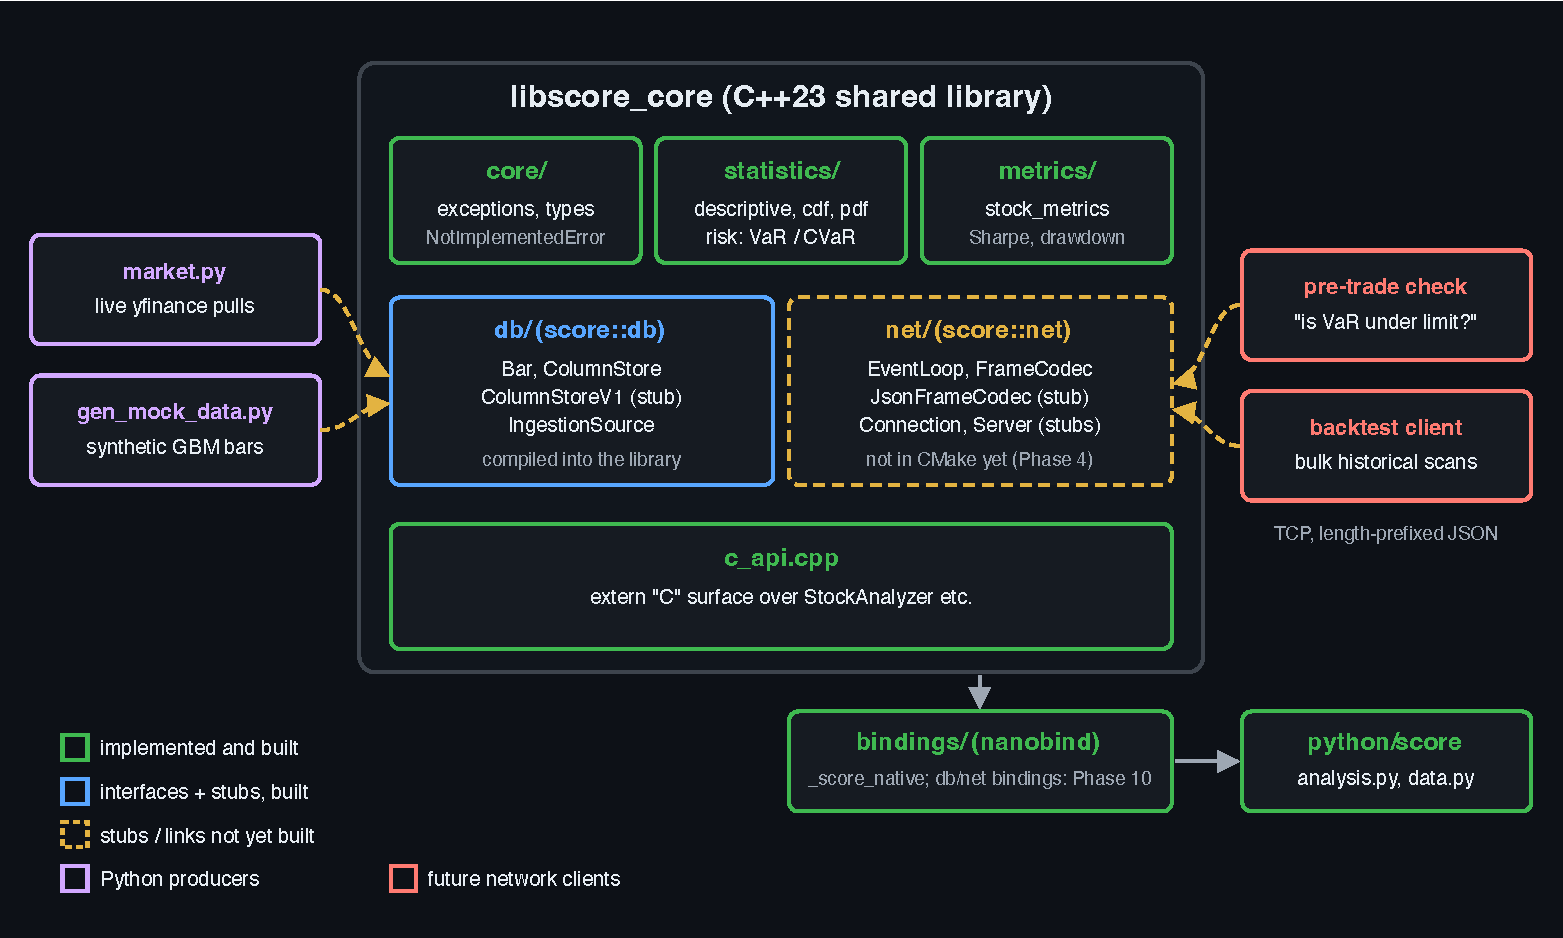
\includegraphics[width=\linewidth]{diagrams/architecture.pdf}
\caption{Module map of \texttt{score} after Phases 0--3 (hand-authored SVG). \texttt{db/} is compiled into the library;
\texttt{net/} exists as headers and stubs but is deliberately not yet in the CMake source list (Phase~4, \cref{ch:roadmap}).}
\label{fig:arch}
\end{figure}

\repopy{src/score/market.py}{\textbf{Data path 1.} \cc{MarketData} wraps \cc{yfinance} and caches one daily-history fetch.
Note \cc{period="1d"}: this facade fetches a single day, so it cannot supply the hundreds of returns a historical VaR
needs. \Cref{ex:yf} asks what \cc{ingest()} must change.}{lst:market}

\repopy[firstline=74,lastline=80]{scripts/gen_mock_data.py}{\textbf{Data path 2} (lines 74--80). The path is the exact
log-space GBM recursion $S_{t+1}=S_t\exp\big((\mu-\tfrac12\sigma^2)\Delta t+\sigma\sqrt{\Delta t}\,Z\big)$ with
$\Delta t=1/252$ (\cref{sec:gbm}). The output is written to JSON and is never read back by the C++ side.}{lst:gbm}

\section{Grilling: interviewing a design into existence}
The request that started this work was roughly ``add a database and some networking, so I can learn''.
That sentence admits thousands of designs, from ``install PostgreSQL and gRPC'' to ``write a kernel-bypass engine''.
A \emph{grilling session} is a structured interview that narrows the space by asking one question at a time,
always with a recommended answer and a reason, until every remaining question has an obvious answer.

\begin{layman}
A good doctor taking a history does not ask every question in the textbook. Each answer prunes the tree:
``does it hurt when you breathe?'' makes some questions urgent and others irrelevant. The doctor also
proposes a working diagnosis at every step, so the patient can say ``no, that's not it''. A grilling session is the
same: each question comes with a proposed answer you can reject.
\end{layman}

\begin{definition}[Decision; falsifier]\label[definition]{def:decision}
A \emph{design decision} is a tuple $(q, A, a^\star, \phi)$: a question $q$, a set of alternatives $A$, the chosen
alternative $a^\star\in A$, and a \emph{falsifier} $\phi$, an observable condition that, if it held, would make some
$a\in A\setminus\{a^\star\}$ the better choice. A decision without a falsifier is a preference, not a decision.
\end{definition}

\begin{definition}[Dependency order and frontier]\label[definition]{def:frontier}
Write $q_i\prec q_j$ if the answer to $q_i$ changes the alternatives available for $q_j$. Given the set $R$ of resolved
questions, the \emph{frontier} is $\mathcal{F}(R)=\{q\notin R:\ \forall p\prec q,\ p\in R\}$.
\end{definition}

The session's one rule is \emph{always ask from the frontier}. Asking a question before its predecessors are settled
wastes the answer: ``epoll or io\_uring?'' is meaningless until ``hand-rolled TCP or gRPC?'' is answered. Because
$\prec$ is acyclic, the frontier is never empty while questions remain, and asking from it is a topological traversal
of the decision graph (\cref{fig:grill}).

\begin{figure}[p]
\centering
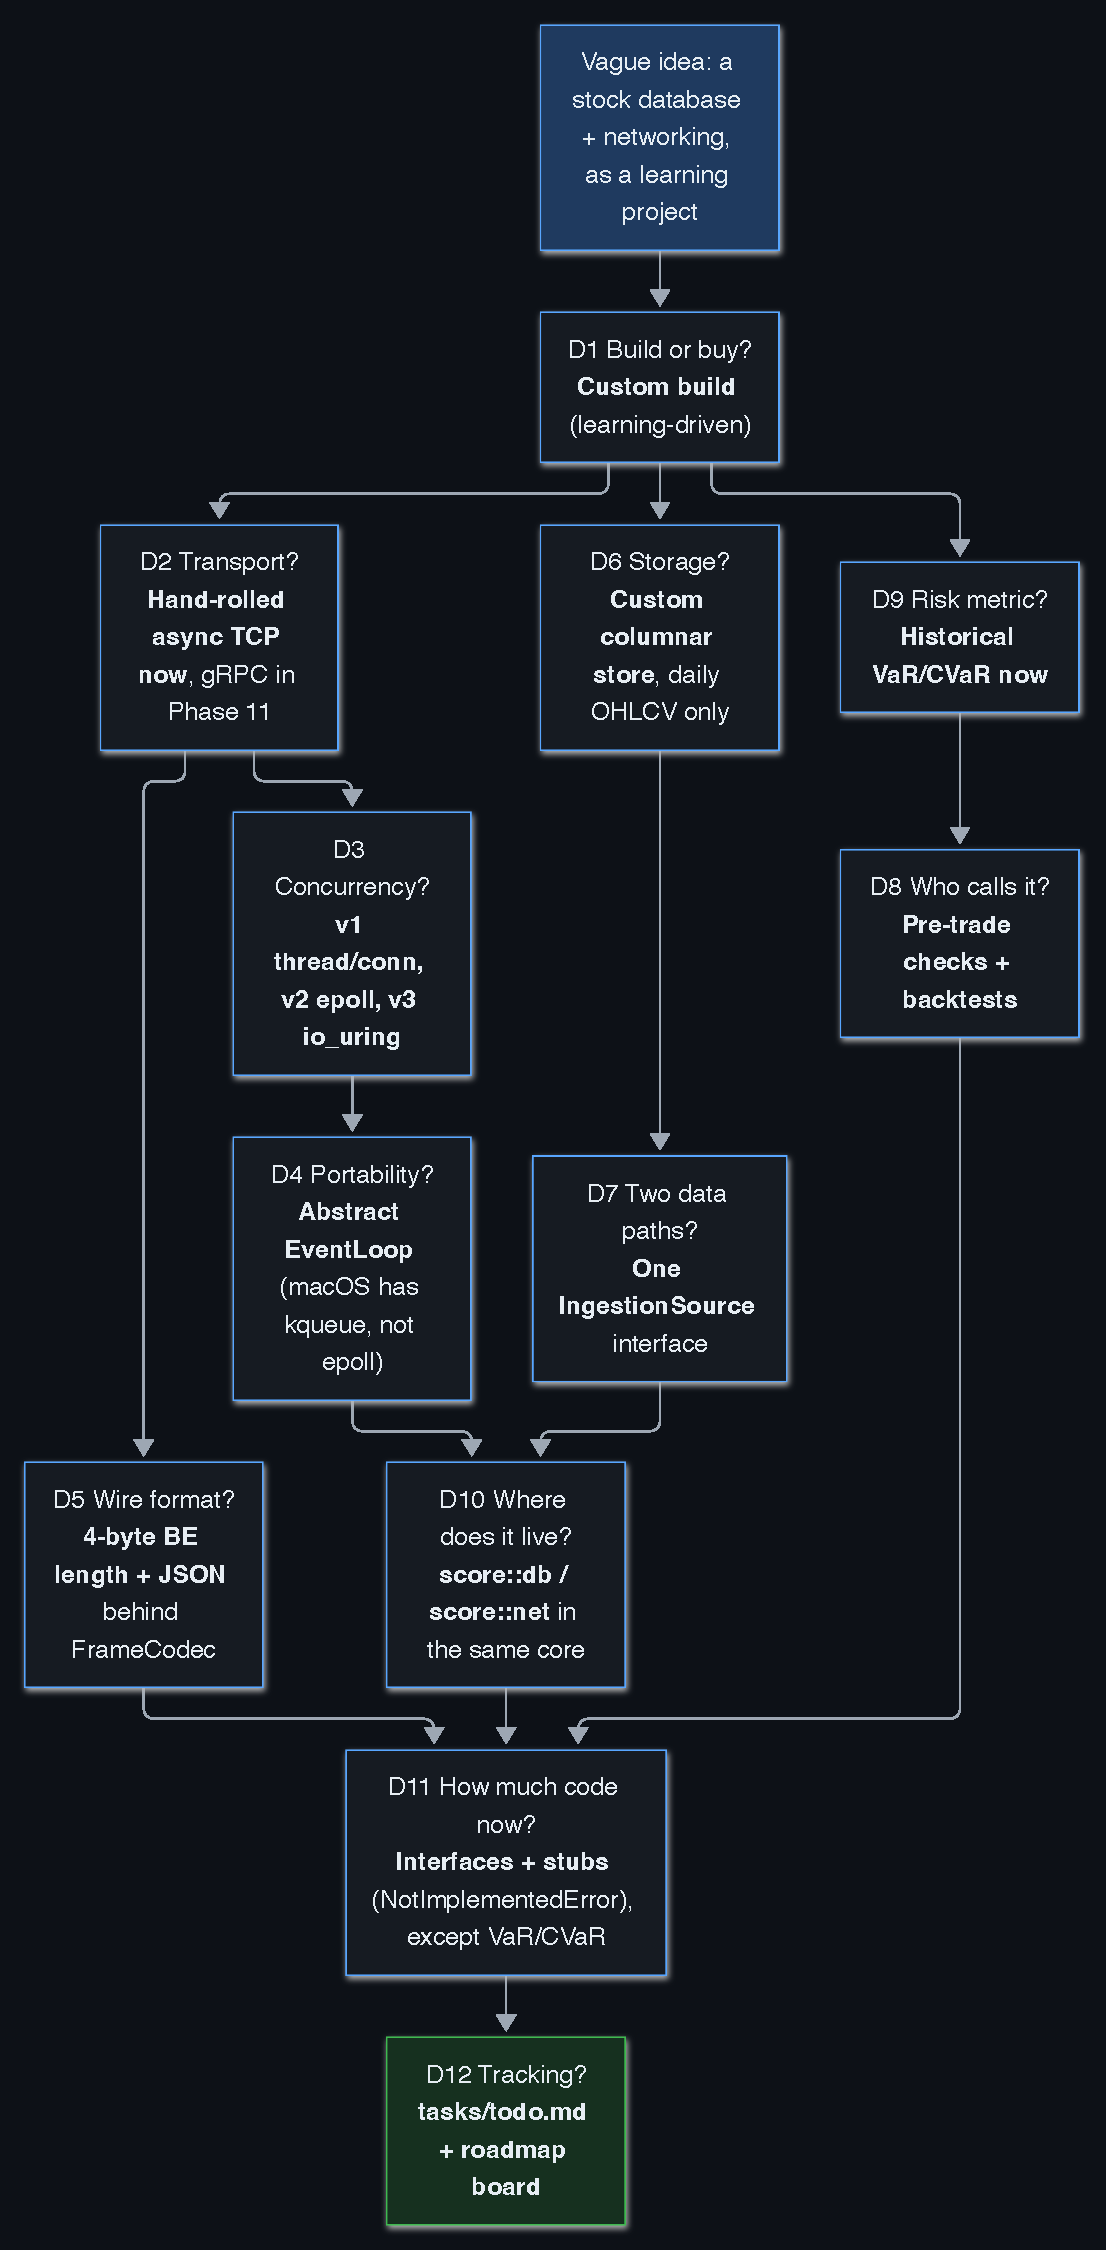
\includegraphics[height=0.82\textheight]{diagrams/grilling.pdf}
\caption{The decision graph of the grilling session (Mermaid). Each node is a question with its recommended answer in
bold. Edges are the dependency relation $\prec$ of \cref{def:frontier}; the session visited nodes in a topological order.}
\label{fig:grill}
\end{figure}

\section{The twelve decisions}
\Cref{tab:decisions} lists the decisions with the alternative that lost and a falsifier for each. Read the
falsifier column carefully: it is the part you will reuse when a decision needs revisiting.

\begin{center}
\footnotesize
\begin{longtable}{@{}>{\leavevmode\bfseries\color{yel}}p{0.6cm} >{\raggedright\arraybackslash}p{3.6cm} >{\raggedright\arraybackslash}p{2.9cm} >{\raggedright\arraybackslash}p{5.4cm}@{}}
\caption{The twelve decisions. ``Lost to'' is the strongest rejected alternative.}\label{tab:decisions}\\
\toprule
\textcolor{muted}{\#} & \textcolor{muted}{Decision} & \textcolor{muted}{Lost to} & \textcolor{muted}{Falsifier (what would reverse it)}\\
\midrule\endfirsthead
\toprule
\textcolor{muted}{\#} & \textcolor{muted}{Decision} & \textcolor{muted}{Lost to} & \textcolor{muted}{Falsifier}\\
\midrule\endhead
D1 & Learning-driven custom build & Off-the-shelf DB + RPC & The goal changes from learning to shipping to users.\\
D2 & Hand-rolled async TCP engine now; gRPC later (Phase 11) & gRPC now & Clients in other languages need the API before Phase 8 is stable.\\
D3 & v1 thread-per-connection $\to$ v2 epoll $\to$ v3 io\_uring (stretch) & Start at epoll & v1 cannot be made correct without the same buffering a reactor needs (\cref{ex:blocking}).\\
D4 & Platform-agnostic \cc{EventLoop} so macOS (kqueue) builds & Linux-only & Development moves entirely to Linux containers.\\
D5 & v1 wire format: 4-byte big-endian length + JSON behind \cc{FrameCodec}; binary later & Binary first & Profiling shows JSON encode/parse dominating request latency.\\
D6 & Custom columnar store, daily OHLCV only & SQLite / Parquet & Intraday or multi-asset data becomes a requirement.\\
D7 & One \cc{IngestionSource} for both data paths & Two ad-hoc loaders & The two sources need incompatible write semantics (e.g.\ corrections that rewrite history).\\
D8 & Users: pre-trade risk checks and backtesting & General analytics & A consumer appears whose queries are not ``one symbol, one date range''.\\
D9 & Real historical VaR/CVaR now & Parametric (Gaussian) VaR & Data too short for the tail ($k=0$, \cref{ch:risk}) at the confidences users ask for.\\
D10 & New \cc{score::db} / \cc{score::net} modules in the same core library & Separate libraries/services & Build times or dependency weight of \texttt{net} hurt Python users who never serve.\\
D11 & Scaffolding only (stubs throw \cc{NotImplementedError}), except VaR/CVaR & Implement everything at once & A stub's interface proves wrong before its implementation phase starts.\\
D12 & Tracked in \file{tasks/todo.md} and the generated roadmap board & Issue tracker & More than one contributor needs to coordinate.\\
\bottomrule
\end{longtable}
\end{center}

\section{Why interfaces first: a counting argument}
Decisions D3, D4 and D5 each name a family of interchangeable implementations: three event loops, two
codecs, two operating systems. Suppose the server were written directly against one concrete loop and one concrete codec.

\begin{proposition}[Sum, not product]\label[proposition]{prop:sum}
Let a component depend on $m$ independent variation points with $v_1,\dots,v_m$ variants each. If it is written against
concrete types, covering all combinations requires $\prod_i v_i$ component variants. If it depends only on an interface per
variation point, it requires one component plus $\sum_i v_i$ implementations.
\end{proposition}
\begin{proof}
Against concrete types, each combination $(a_1,\dots,a_m)$ fixes the source text of the component, and distinct
combinations give distinct texts, hence $\prod_i v_i$ variants. Against interfaces, the component's text mentions no
variant; each variant is written once, behind its interface, and any combination is assembled at construction time
(for \cc{Server}: an \cc{EventLoop&} and a \cc{CodecFactory}). That is $1+\sum_i v_i$ units of code.
\end{proof}

For \texttt{score}, with $v=(3,2)$ for (event loop, codec), that is $6$ server variants versus $1+5$ units, and the gap
widens with every new backend. Parnas made the underlying argument in 1972: decompose a system so that each module
hides one \emph{design decision likely to change}~\cite{parnas1972criteria}. \cc{EventLoop} hides the concurrency model,
\cc{FrameCodec} the wire format, \cc{ColumnStore} the byte layout, \cc{IngestionSource} the provenance of the data.
Martin later named the same idea the Dependency Inversion Principle~\cite{martin2003agile}.

\begin{remarkbox}
Interfaces are not free. Every call through \cc{EventLoop} is a virtual call, and every \cc{IoCallback} is a
\cc{std::function} that may allocate. For a learning project those costs are noise next to a system call, which is
two to three orders of magnitude more expensive (\cref{tab:costs}). Measure before removing them.
\end{remarkbox}

\section{Scaffolding that fails loudly}
Decision D11 says that everything except VaR/CVaR is scaffolding: real headers, real class shapes, and bodies that throw.

\repo[firstline=31,lastline=34]{include/score/core/exceptions.hpp}{The exception every stub throws (lines 31--34). It derives from
\cc{ScoreException}, which derives from \cc{std::runtime_error}, so Python callers see an ordinary exception
once bindings exist.}{lst:notimpl}

\repo{src/net/json_codec.cpp}{A typical stub. Every method throws; none returns a plausible default.}{lst:jsonstub}

\begin{claim}\label[claim]{claim:loud}
A stub that throws is strictly safer than a stub that returns a default value of the declared type.
\end{claim}
\begin{proof}[Argument]
Consider \cc{try_decode()} returning \cc{std::nullopt} as a ``harmless'' default. Every caller treats
\cc{nullopt} as ``not enough bytes yet'', so a test that feeds a complete frame and asserts nothing more than ``no crash''
passes, and a server built on it silently never answers. A throwing stub turns the same test into a failure, and its
message names the unimplemented function. A test can only pass against a throwing stub if it never calls the stub, and that
is visible in coverage. So the throwing stub cannot produce a vacuous pass, while the defaulting stub can.
\end{proof}

\begin{history}
Brooks's advice to ``plan to throw one away''~\cite{brooks1975mythical} is often quoted as permission to write disposable
code. Scaffolding is the opposite bet: keep the \emph{interfaces}, which are cheap to get right by thinking,
and postpone the \emph{implementations}, which are cheap to get right only by building. The grilling session existed to make the
interfaces right before any implementation existed.
\end{history}

\begin{exercises}
\ex{ex:falsify}{\lvA} For decisions D2, D6 and D9, describe a concrete measurement or event in \emph{this} repository that
would trigger the falsifier in \cref{tab:decisions}. Who would observe it, and in which file?

\ex{ex:leak}{\lvB} Parnas's criterion says an interface should hide one secret. \cc{event_loop.hpp} declares
\cc{using SocketHandle = int;}. Which secret leaks through that line? What breaks on Windows, where a socket is
\cc{SOCKET}, an unsigned pointer-sized integer? Propose a fix that does not add a virtual call.

\ex{ex:order}{\lvB} \cc{ColumnStore::append} documents that implementations ``should reject bars that are out of
order or overlap dates already stored''. The interface cannot enforce this. Sketch a type (for example a
\cc{SortedBars} that can only be built by a validating factory) that makes an unsorted batch unrepresentable, and
discuss what it costs at the Python boundary.

\ex{ex:lifetime}{\lvB} \cc{Connection} stores \cc{EventLoop& loop_}, and its destructor is defaulted, while
\cc{close()} must unregister from the loop. Specify the destruction order of \cc{Server}, its \cc{connections_}, and the
loop so that no callback can run on a destroyed \cc{Connection}. Which of the three may outlive the others?

\ex{ex:frontier}{\lvC} \Cref{fig:grill} is one topological order. Find a pair of decisions whose order in the session
could be swapped without changing any answer, and a pair that could not. Then argue whether a design interview
should prefer depth-first (finish a branch) or breadth-first (settle every top-level question first) traversal of the frontier.
\end{exercises}


\chapter{TCP and Sockets: A Byte Stream, Not a Message Queue}\label{ch:tcp}

\begin{objectives}
\begin{itemize}
\item state TCP's service model precisely, including what it does \emph{not} promise;
\item walk the \cc{socket}/\cc{bind}/\cc{listen}/\cc{accept} lifecycle and say which kernel object each call creates;
\item explain the listen backlog and the two queues behind it;
\item prove that any protocol relying on \cc{recv} boundaries is incorrect, and reproduce the failure on loopback;
\item map each call onto \cc{Server::listen}, \cc{Connection}, and \cc{SocketHandle} in \texttt{score::net}.
\end{itemize}
{\small\color{muted}\textbf{Chapter references:} RFC 793 and RFC 9293~\cite{rfc793,rfc9293}; RFC 896~\cite{rfc896}; RFC 1122~\cite{rfc1122};
Stevens et al.~\cite{stevens2004unp}; Kerrisk~\cite{kerrisk2010tlpi}.}
\end{objectives}

\section{The service model}
TCP was specified in RFC~793 (1981)~\cite{rfc793} and consolidated in RFC~9293 (2022)~\cite{rfc9293}. Its promise to an
application is narrow, and most networking bugs come from assuming more than it gives.

\begin{definition}[Reliable byte stream]\label[definition]{def:bytestream}
A \emph{reliable byte stream} from $A$ to $B$ is a channel such that, if $A$ writes the byte sequences
$w_1, w_2, \dots, w_m$, then the concatenation of everything $B$ reads is a prefix of $w_1\Vert w_2\Vert\cdots\Vert w_m$,
and, absent failure, eventually the whole of it. Nothing is promised about how the bytes are grouped into reads.
\end{definition}

TCP provides two such streams per connection, one in each direction (full duplex). It handles loss, duplication and
reordering in the network with sequence numbers, acknowledgements and retransmission. It does \emph{not} carry the
application's write boundaries: a write is not a message, and a segment is not a write.

\begin{layman}
UDP is like posting letters: each envelope arrives whole or not at all, possibly out of order. TCP is like a garden
hose: the water arrives in order, but nobody can tell from the water where one bucketful ended and the next began. If
you need buckets, you have to mark them yourself. That marking is \emph{framing} (\cref{ch:framing}).
\end{layman}

\begin{proposition}[Boundary-blindness]\label[proposition]{prop:boundary}
Let $S=w_1\Vert\cdots\Vert w_m$ with $|S|=B$. Under \cref{def:bytestream}, any sequence of positive integers
$(\ell_1,\dots,\ell_q)$ with $\sum_j\ell_j=B$ is a permissible sequence of \cc{recv} return values (subject only to
each $\ell_j$ not exceeding the receiver's buffer size). Consequently an application protocol whose parsing depends on
the $\ell_j$ is not correct over TCP.
\end{proposition}
\begin{proof}
The definition constrains only the \emph{content} of the concatenated reads, never their lengths, so every
composition of $B$ is consistent with it. A protocol is correct only if it behaves correctly on every permitted
execution. If its output depends on $(\ell_j)$, two executions with equal byte content but different compositions give
different outputs, so at least one is wrong.
\end{proof}

The proposition is not hypothetical. \Cref{lst:streamdemo} writes one 44-byte frame (the one we will dissect in
\cref{ch:framing}) as three \cc{send} calls of 3, 20 and 21 bytes over loopback, with \cc{TCP_NODELAY} set, first with
50\,ms pauses and then with none.

\begin{code}{stream\_demo.cpp (excerpt): one frame, three writes}{lst:streamdemo}
const int cuts[] = {0, 3, 23, 44};
for (int i = 0; i < 3; ++i) {
    send(c, frame + cuts[i], cuts[i + 1] - cuts[i], 0);
    std::this_thread::sleep_for(std::chrono::milliseconds(pause_ms));
}
// ... server side, after accept():
for (ssize_t n; (n = recv(fd, buf, sizeof buf, 0)) > 0;) std::printf(" %zd", n);
\end{code}

\begin{progout}{stream\_demo on macOS loopback (two runs, identical)}{lst:streamout}
writes 3+20+21 with 50 ms pauses -> recv() returned: 3 20 21 0 (EOF)
writes 3+20+21 with 0 ms pauses -> recv() returned: 44 0 (EOF)
\end{progout}

The same bytes produced the read compositions $(3,20,21)$ and $(44)$ depending only on timing. A parser that
assumed ``one \cc{recv} = one request'' would see three garbage requests in the first run and be right only by luck in
the second. Over a real network, with a different maximum segment size, retransmissions and receive-window updates, the
compositions vary even more.

\section{The socket lifecycle}
A server needs a \emph{listening} socket, which never carries data, and one \emph{connected} socket per client.
\Cref{fig:tcp} shows the calls and the three-way handshake between them.

\begin{figure}[htbp]
\centering
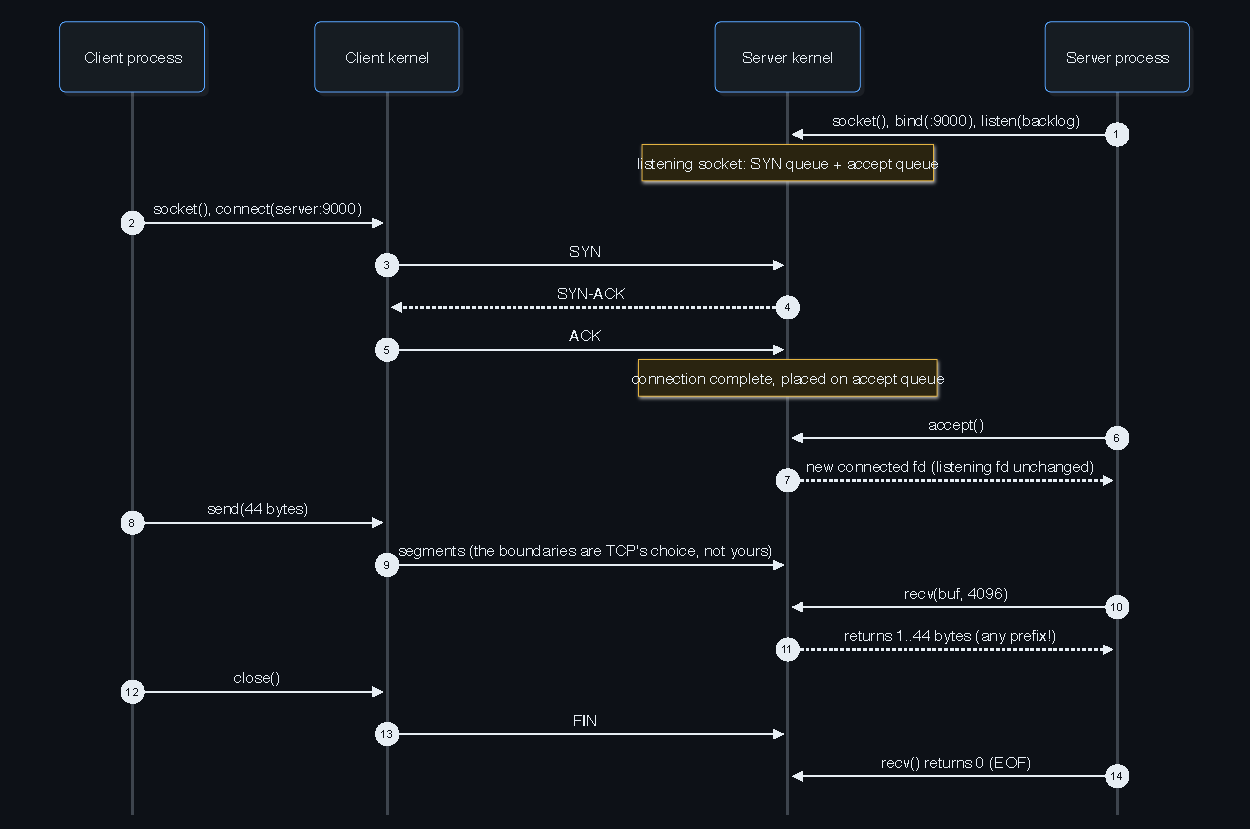
\includegraphics[width=\linewidth]{diagrams/tcp_lifecycle.pdf}
\caption{Server and client socket lifecycle, with the handshake performed by the kernels (Mermaid). The server process
is not involved in the handshake: \cc{accept} only dequeues a connection that the kernel has already completed.}
\label{fig:tcp}
\end{figure}

\begin{center}
\small
\begin{tabularx}{\linewidth}{@{}>{\leavevmode\ttfamily\color{org}}l X@{}}
\toprule
\textcolor{muted}{\rmfamily Call} & \textcolor{muted}{What it does in the kernel}\\
\midrule
socket(AF\_INET, SOCK\_STREAM, 0) & Allocates a socket object and returns a descriptor, a small integer indexing the process's file table. In \texttt{score} this is \cc{SocketHandle = int}.\\
setsockopt(SO\_REUSEADDR) & Allows \cc{bind} to an address with old connections still in TIME-WAIT, so a restarted server can rebind at once.\\
bind(fd, addr) & Attaches a local address and port.\\
listen(fd, backlog) & Marks the socket passive. The kernel now completes handshakes on its behalf and queues finished connections.\\
accept(fd) & Dequeues one completed connection and returns a \emph{new} descriptor for it. The listening descriptor is unchanged.\\
connect(fd, addr) & Client side: starts the handshake (SYN) and returns when it completes or fails.\\
recv / send & Copy bytes between user memory and the socket's kernel buffers. Either may move fewer bytes than asked.\\
shutdown(fd, SHUT\_WR) & Sends FIN (``I will write no more'') while still allowing reads: a half-close.\\
close(fd) & Releases the descriptor; the kernel finishes the connection teardown.\\
\bottomrule
\end{tabularx}
\end{center}

\subsection{The listen backlog}
The kernel holds two kinds of not-yet-accepted connections: those mid-handshake (SYN received, SYN-ACK sent) and those
complete but not yet returned by \cc{accept}. On Linux the \cc{backlog} argument bounds the second queue, the
\emph{accept queue}, and is silently capped by \cc{net.core.somaxconn}; half-open connections are governed separately by
\cc{tcp_max_syn_backlog}~\cite{kerrisk2010tlpi}. On the measurement machine, \cc{sysctl kern.ipc.somaxconn} reports
\texttt{128}. If the accept queue is full because the application is slow to call \cc{accept}, new clients see their SYNs
dropped or refused and retry with exponential back-off, which shows up as latency spikes of whole seconds rather than as
errors.

\begin{remarkbox}
The backlog is where the concurrency model of \cref{ch:conc} becomes visible to clients. A thread-per-connection server
calls \cc{accept} in a loop and hands off immediately, so its accept queue drains quickly until the machine runs out of
threads. A reactor calls \cc{accept} when the listening descriptor is reported \emph{readable}, so a slow handler on the
loop thread delays every \cc{accept}.
\end{remarkbox}

\section{Partial reads, partial writes, and the errors in between}
\Cref{prop:boundary} applies to writes too: \cc{send} on a non-blocking socket may accept fewer bytes than requested
when the kernel send buffer is nearly full, and then fails with \cc{EAGAIN} until space frees up. Correct code therefore
has the same shape on both sides:

\begin{code}{write\_all: the loop every sender needs (blocking socket)}{lst:writeall}
bool write_all(int fd, const std::uint8_t* p, std::size_t n) {
    while (n > 0) {
        ssize_t k = ::send(fd, p, n, 0);
        if (k < 0) {
            if (errno == EINTR) continue;   // interrupted by a signal: retry
            return false;                   // real error (EPIPE, ECONNRESET, ...)
        }
        p += k;                              // k may be < n: advance and loop
        n -= static_cast<std::size_t>(k);
    }
    return true;
}
\end{code}

On a non-blocking socket the reactor version cannot loop: on \cc{EAGAIN} it must keep the unsent tail in a per-connection
output buffer and register for \cc{IoEvent::kWritable}. That is precisely why \cc{Connection::send} is documented as
``\emph{queues} \cc{frame} for writing''.

\repo[firstline=9,lastline=29]{include/score/net/connection.hpp}{\cc{Connection} owns the descriptor and a codec and
holds a reference to the loop. The word ``queues'' in the comment on \cc{send} commits the implementation to an output
buffer, because a non-blocking write may be partial.}{lst:connection}

\subsection{Small writes and Nagle's algorithm}
Nagle's algorithm (RFC~896, 1984)~\cite{rfc896} holds back a small segment while earlier data is unacknowledged, and
receivers commonly delay ACKs~\cite{rfc1122}. A sender that writes a 4-byte length prefix and then the payload as
\emph{two} writes can stall for a delayed-ACK interval waiting for an acknowledgement. Two habits avoid it:
build the whole frame in one buffer (as \cc{FrameCodec::encode} does by returning a single \cc{std::vector<std::uint8_t>}),
or use a gather write (\cc{writev}). Setting \cc{TCP_NODELAY} disables Nagle's algorithm but does not make two writes
one.

\section{Mapping onto \texttt{score::net}}
\repo[firstline=13,lastline=38]{include/score/net/server.hpp}{\cc{Server::listen(port)} will be
\cc{socket}+\cc{setsockopt}+\cc{bind}+\cc{listen}, then registration of the listening descriptor with the loop for
readability. Each readable event on it means ``\cc{accept} will not block''. Each accepted descriptor gets a fresh codec
from \cc{CodecFactory}, because codecs hold per-connection buffers.}{lst:server}

\begin{example}[One request, end to end]\label[example]{ex:e2e}
A pre-trade client connects, writes the 44-byte frame of \cref{fig:frame} and waits. The server kernel completes the
handshake and queues the connection; the loop reports the listening descriptor readable; \cc{Server} calls \cc{accept}
and creates a \cc{Connection} with a new \cc{JsonFrameCodec}; the loop later reports the connection readable; the
callback \cc{recv}s some prefix of the 44 bytes and \cc{feed}s it to the codec; \cc{try_decode} returns \cc{nullopt}
until all 44 bytes have arrived (\cref{thm:segmentation}); the handler computes VaR and \cc{send}s a reply frame, which
may itself take several writes.
\end{example}

\begin{exercises}
\ex{ex:listen}{\lvA} Write the exact sequence of system calls \cc{Server::listen(9000)} should make, including
\cc{SO_REUSEADDR}, \cc{O_NONBLOCK} and the loop registration. Say what goes wrong in a test suite that restarts the
server on the same port if \cc{SO_REUSEADDR} is omitted.

\ex{ex:compositions}{\lvB} A client sends two 44-byte frames back to back. How many distinct \cc{recv} return sequences
are possible if the server's buffer is 64 bytes? Which of them leave the second frame's length prefix split across two
reads? (Count compositions with bounded parts.)

\ex{ex:sendq}{\lvB} \cc{Connection::send} is called from a request handler while the kernel send buffer is full. Design the
output queue: data structure, when to register and unregister \cc{kWritable}, and a cap that stops a slow reader from
exhausting server memory. What should happen to the connection when the cap is hit?

\ex{ex:backlog}{\lvC} With the accept queue full, what exactly does a client observe on Linux, and what on macOS?
Design an experiment with a server that never calls \cc{accept}, and predict the client's \cc{connect} latency
distribution before running it.

\ex{ex:halfclose}{\lvB} A backtest client sends 500 requests and then has nothing more to say, but still needs the 500
replies. Explain how \cc{shutdown(SHUT_WR)} helps the server, and what the server's read loop sees.
\end{exercises}


\chapter{Concurrency Models: Threads, Readiness and Completion}\label{ch:conc}

\begin{objectives}
\begin{itemize}
\item build a cost model for thread-per-connection (stack memory, context switches) and evaluate it with measured numbers;
\item prove that \cc{select}/\cc{poll} cost $\Theta(n)$ per call and that \cc{epoll}/\cc{kqueue} cost $\Theta(1+r)$, and check both against a benchmark;
\item distinguish the reactor and proactor patterns, and say which one \cc{score::net::EventLoop} is;
\item explain io\_uring's submission and completion rings;
\item map v1, v2 and v3 of the roadmap onto the \cc{EventLoop} interface and its limits.
\end{itemize}
{\small\color{muted}\textbf{Chapter references:} Kegel~\cite{kegel1999c10k}; Banga et al.~\cite{banga1999scalable}; Lemon~\cite{lemon2001kqueue};
Schmidt~\cite{schmidt1995reactor}; Pyarali et al.~\cite{pyarali1997proactor}; POSA2~\cite{schmidt2000posa2};
Axboe~\cite{axboe2019iouring}; Kerrisk~\cite{kerrisk2010tlpi}.}
\end{objectives}

\section{The question: how does one process serve \texorpdfstring{$n$}{n} connections?}
A connection spends nearly all its life waiting: for the client to send, for the kernel to free buffer space, for a
disk. Concurrency models differ in \emph{who waits} and \emph{what waiting costs}. There are three families:
\begin{enumerate}[label=\textbf{\color{yel}(\roman*)}]
\item \textbf{One thread per connection.} Each thread blocks in \cc{recv}; the kernel scheduler is the event loop.
\item \textbf{Readiness notification (reactor).} One thread asks the kernel ``which of my descriptors can make progress?'' and performs non-blocking I/O on those.
\item \textbf{Completion notification (proactor).} The thread submits operations; the kernel performs them and reports ``this read finished, here are the bytes''.
\end{enumerate}

\begin{history}
In 1999 Dan Kegel's web page ``The C10K problem''~\cite{kegel1999c10k} asked how to serve ten thousand concurrent clients
from one machine, and catalogued the then-available strategies. At the time the dominant Apache configuration,
the \emph{prefork} model, dedicated a whole process to each connection. Banga, Mogul and Druschel had just shown that
\cc{select}'s per-call cost made event-driven servers scale poorly and proposed an explicit event-delivery
interface~\cite{banga1999scalable}. FreeBSD's \cc{kqueue} (Lemon, 2001)~\cite{lemon2001kqueue} and Linux's \cc{epoll}
(merged during the 2.5 development series, first stable in 2.6) followed. nginx, publicly released by Igor Sysoev in 2004,
was built around such an event loop from the start. \Cref{sec:hist-c10k} returns to this history.
\end{history}

\section{Thread-per-connection: the cost model}\label{sec:tpc}
\begin{layman}
A restaurant can give every table its own waiter. Service is simple, since each waiter only thinks about one table, but
waiters stand idle most of the evening, every one of them needs a uniform and a locker, and when twenty waiters crowd the
kitchen door they spend their time getting out of each other's way.
\end{layman}

Let $n$ be the number of connections. Each thread needs a stack (virtual address space reserved up front, physical
pages committed on first touch) and kernel bookkeeping, and each request wakes a thread, which costs a context switch.

\begin{definition}[Thread-per-connection cost model]\label[definition]{def:tpcmodel}
With reserved stack size $S$, resident stack $s\le S$, per-thread kernel overhead $\kappa$, service time $w$ per request and
context-switch cost $\sigma$, a thread-per-connection server needs virtual memory $V(n)=nS$, resident memory
$M(n)\approx n(s+\kappa)$, and on one core can complete at most
\[ \lambda_{\max}=\frac{1}{w+2\sigma} \]
requests per second, counting one switch to wake the handler and one to leave it.
\end{definition}

\begin{verified}
Measured on the machine described on the title page (\file{verify/layout.cpp}, \file{verify/bench.cpp}):
\begin{itemize}
\item default \cc{pthread} stack for a secondary thread: \textbf{524{,}288 bytes (512 KiB)}; \cc{ulimit -s} for the main thread: \textbf{8176 KiB};
\item \cc{std::thread} create + join: \textbf{14.9\,\textmu s} (mean of 20{,}000);
\item one blocking hand-off between two threads over a pipe (half a ping-pong round trip): \textbf{2.3\,\textmu s} (mean of 200{,}000 round trips of 4.5\,\textmu s).
\end{itemize}
\end{verified}

With $S=512$\,KiB, $10^4$ threads reserve $4.88$\,GiB of address space; with the 8\,MiB default common on Linux, $78.1$\,GiB.
Reservation is not residence, so the machine survives, but the numbers explain why thread-per-connection servers lower
the stack size. The switching term matters more: if $w$ is a few microseconds of VaR arithmetic on cached data, then
$2\sigma\approx 4.6$\,\textmu s is the same order as the useful work.

\section{Readiness APIs and their asymptotics}
\subsection{select and poll: the interest set travels on every call}
\cc{poll(fds, n, timeout)} receives an array of $n$ descriptors each time it is called. \cc{select} does the same with
bitmaps limited to \cc{FD_SETSIZE} descriptors (1024 on this system, verified by compiling a one-line program).

\begin{proposition}[Linear cost of stateless readiness]\label[proposition]{prop:polln}
Any implementation of \cc{poll} that holds no state between calls takes $\Omega(n)$ time per call, even if only one
descriptor is ready.
\end{proposition}
\begin{proof}
The result must report \cc{revents} for every entry, and the input may differ arbitrarily from the previous call. An
implementation that skipped entry $i$ could not distinguish an input where descriptor $i$ is ready from one where it is
not, so it would be wrong on one of them. Hence every entry is read, and copying the array from user memory alone is $\Theta(n)$.
\end{proof}

\subsection{epoll and kqueue: the interest set lives in the kernel}
\cc{epoll_ctl} and \cc{kevent} \emph{register} interest once. The kernel attaches a callback to each watched file, and
when a file becomes ready the callback appends it to a ready list. \cc{epoll_wait} and \cc{kevent} only drain that list.

\begin{theorem}[Cost of stateful readiness]\label{thm:epoll}
If registering and deregistering a descriptor costs $O(1)$ amortized, and each readiness transition costs $O(1)$ to record,
then a wait that returns $r$ ready descriptors costs $\Theta(1+r)$, independent of the number $n$ of registered descriptors.
\end{theorem}
\begin{proof}[Proof sketch]
The wait performs constant work to check the ready list and $O(1)$ per element it copies out, giving $O(1+r)$. It must at least
write $r$ results, giving $\Omega(1+r)$. The $n$ idle descriptors are never touched by the wait: their cost was paid once
at registration and is charged to \cc{epoll_ctl}/\cc{kevent} calls, not to waits. Summed over a run, total work is
$O(\#\text{registrations}+\#\text{transitions}+\sum r)$.
\end{proof}

The prediction is easy to test: register $n$ pipes, make exactly one readable, and time a zero-timeout wait.
\Cref{fig:pollbench} shows the result.

\begin{figure}[htbp]
\centering
\begin{tikzpicture}
\begin{loglogaxis}[darkaxis,width=0.92\linewidth,height=7.2cm,
  xlabel={registered descriptors $n$ (one ready)},ylabel={time per call (\textmu s)},
  grid=major,legend pos=north west,xmin=0.8,xmax=12000,ymin=0.1,ymax=3000]
\addplot[color=red,mark=*,mark size=1.8pt,thick] table[x=n,y=poll_us]{data/bench.dat};
\addlegendentry{\texttt{poll()} (interest set copied each call)}
\addplot[color=grn,mark=square*,mark size=1.8pt,thick] table[x=n,y=kqueue_us]{data/bench.dat};
\addlegendentry{\texttt{kevent()} on a \texttt{kqueue} (registered once)}
\addplot[color=muted,dashed,domain=1:10000,samples=2] {0.1394*x};
\addlegendentry{fit: $0.139\,n$ \textmu s}
\end{loglogaxis}
\end{tikzpicture}
\caption{Measured cost of one readiness check on macOS (Apple M3 Max), median of five runs of 2000 calls
(\file{verify/bench.cpp}). \texttt{poll} grows linearly, about 0.139\,\textmu s per descriptor (least-squares fit);
\texttt{kevent} stays near 0.19--0.24\,\textmu s from $n=1$ to $n=8000$.}
\label{fig:pollbench}
\end{figure}

\begin{center}
\small
\begin{tabular}{@{}rrrr@{}}
\toprule
\textcolor{muted}{$n$} & \textcolor{muted}{\texttt{poll} (\textmu s)} & \textcolor{muted}{\texttt{kevent} (\textmu s)} & \textcolor{muted}{ratio}\\
\midrule
1 & 0.386 & 0.197 & 2.0\\
100 & 11.378 & 0.200 & 57\\
1000 & 134.507 & 0.197 & 683\\
8000 & 1106.619 & 0.200 & 5533\\
\bottomrule
\end{tabular}
\end{center}

\subsection{Level- versus edge-triggered}
In \emph{level-triggered} mode (the default for both APIs) a descriptor is reported on every wait while it remains readable.
In \emph{edge-triggered} mode (\cc{EPOLLET}, \cc{EV_CLEAR}) it is reported once per transition from not-ready to ready.

\begin{pitfall}[title={Pitfall: edge-triggered without draining}]
With edge triggering, a handler that reads 4096 bytes and returns while more bytes sit in the socket buffer will
not be told again until \emph{new} data arrives. If the client is waiting for a reply before sending more, both sides
wait forever. Under edge triggering the rule is: read until \cc{EAGAIN}, and feed everything to the codec.
\Cref{ex:et} asks you to prove the deadlock.
\end{pitfall}

\section{Reactor and proactor}
Schmidt named the readiness pattern the \emph{Reactor}~\cite{schmidt1995reactor}; Pyarali, Harrison, Schmidt and Jordan
named the completion pattern the \emph{Proactor}~\cite{pyarali1997proactor}; both are catalogued in
POSA2~\cite{schmidt2000posa2}.

\begin{definition}[Reactor]\label[definition]{def:reactor}
An event loop that demultiplexes \emph{readiness} events on a set of handles and synchronously dispatches each to a
registered handler, which then performs the I/O itself without blocking.
\end{definition}
\begin{definition}[Proactor]\label[definition]{def:proactor}
An event loop in which handlers \emph{initiate} asynchronous operations, the operating system performs them, and the loop
dispatches \emph{completion} events, carrying results, to completion handlers.
\end{definition}

\begin{figure}[htbp]
\centering
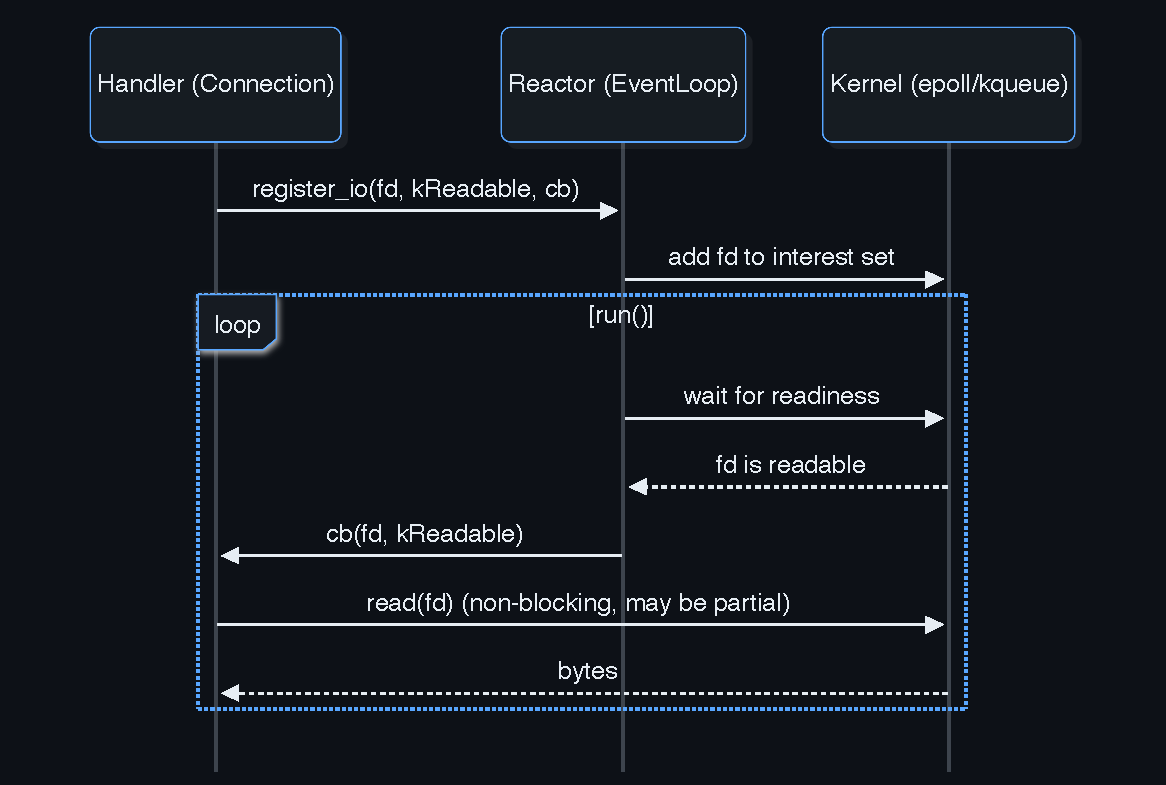
\includegraphics[width=0.66\linewidth]{diagrams/reactor_seq.pdf}\\[-1pt]
{\small\color{muted}(a) Reactor: ``you may read now''.}\\[6pt]
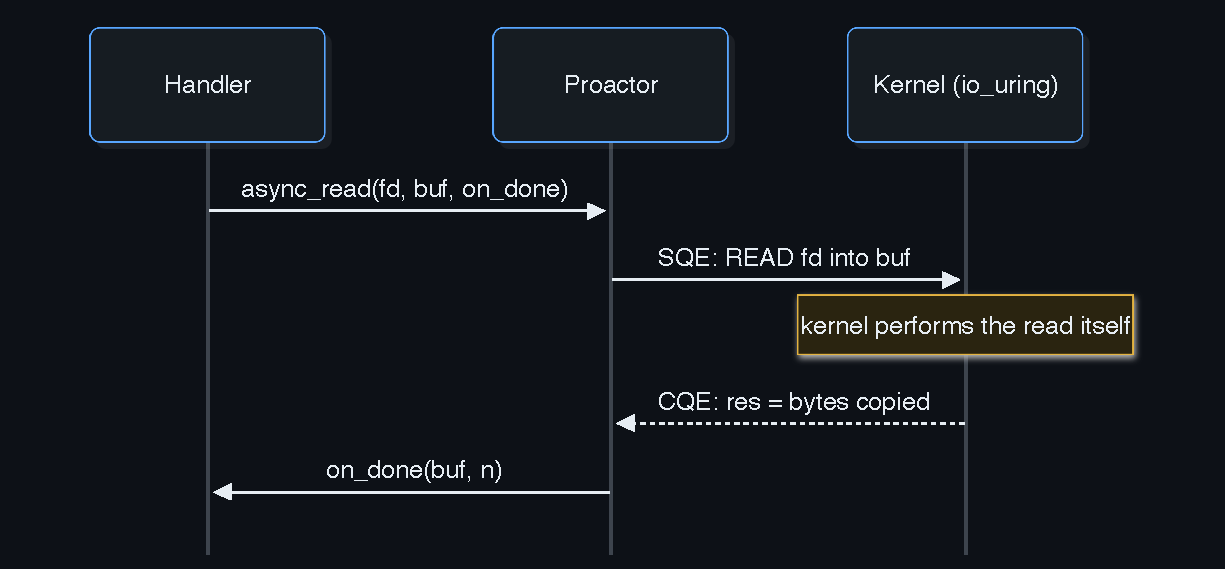
\includegraphics[width=0.6\linewidth]{diagrams/proactor_seq.pdf}\\[-1pt]
{\small\color{muted}(b) Proactor: ``your read is done''.}
\caption{Readiness versus completion (Mermaid). In (a) the handler performs the copy; in (b) the kernel does, into a
buffer the handler supplied when it submitted the operation.}
\label{fig:reactorproactor}
\end{figure}

\repo[firstline=5,lastline=34]{include/score/net/event_loop.hpp}{\cc{EventLoop} is a \emph{reactor} interface:
\cc{register_io(fd, event, cb)} subscribes to readiness, and \cc{IoCallback} receives only \cc{(fd, event)}, no bytes and
no byte count. A completion backend must therefore either emulate readiness or the interface must grow
(\cref{ex:uringadapt}).}{lst:eventloop}

\section{io\_uring: shared rings}
io\_uring, designed by Jens Axboe and merged in Linux 5.1 (2019)~\cite{axboe2019iouring}, replaces one system call per
operation with two ring buffers in memory shared between the process and the kernel. The application writes
\emph{submission queue entries} (SQEs) at the tail of the SQ; the kernel consumes them from the head, performs the
operations, and writes \emph{completion queue entries} (CQEs) to the CQ, which the application consumes.

\begin{figure}[htbp]
\centering
\begin{tikzpicture}[x=0.9cm,y=0.9cm]
  % SQ
  \node[font=\small\bfseries,text=acc] at (3.5,2.0) {Submission queue (SQ)};
  \foreach \i in {0,...,7}{\draw[draw=acc,fill=codebg] (\i,0.6) rectangle ++(1,0.9);}
  \foreach \i/\t in {2/READ,3/READ,4/WRITE}{\fill[acc!35!codebg] (\i+0.04,0.64) rectangle ++(0.92,0.82); \node[font=\scriptsize\ttfamily,text=fg] at (\i+0.5,1.05) {\t};}
  \draw[-{Stealth},thick,yel] (2.0,-0.1) node[below,font=\scriptsize,text=yel]{head (kernel)} -- (2.0,0.55);
  \draw[-{Stealth},thick,grn] (5.0,-0.1) node[below,font=\scriptsize,text=grn]{tail (app)} -- (5.0,0.55);
  % CQ
  \node[font=\small\bfseries,text=org] at (13.0,2.0) {Completion queue (CQ)};
  \foreach \i in {0,...,7}{\draw[draw=org,fill=codebg] (9.5+\i,0.6) rectangle ++(1,0.9);}
  \foreach \i/\t in {1/res=44,2/res=4096}{\fill[org!35!codebg] (9.5+\i+0.04,0.64) rectangle ++(0.92,0.82); \node[font=\tiny\ttfamily,text=fg] at (9.5+\i+0.5,1.05) {\t};}
  \draw[-{Stealth},thick,grn] (10.5,-0.1) node[below,font=\scriptsize,text=grn]{head (app)} -- (10.5,0.55);
  \draw[-{Stealth},thick,yel] (12.5,-0.1) node[below,font=\scriptsize,text=yel]{tail (kernel)} -- (12.5,0.55);
  % kernel
  \node[boxn,draw=muted,minimum width=4.8cm] (k) at (8.25,-1.9) {kernel: consume SQEs, perform I/O, post CQEs};
  \draw[arr] (4.0,0.55) to[out=-90,in=150] (k.west);
  \draw[arr] (k.east) to[out=30,in=-90] (12.0,0.55);
  \node[font=\scriptsize,text=muted,align=center] at (8.25,1.05) {shared\\memory};
\end{tikzpicture}
\caption{io\_uring's two single-producer/single-consumer rings (TikZ). The application produces SQEs and consumes CQEs;
the kernel does the reverse. One \texttt{io\_uring\_enter} call can submit many SQEs; in \texttt{SQPOLL} mode a kernel
thread polls the SQ and submission needs no system call at all.}
\label{fig:uring}
\end{figure}

Because each ring has exactly one producer and one consumer, it needs no lock: the producer writes the entry, then
publishes it by storing the new tail with release semantics; the consumer reads the tail with acquire semantics before
reading entries. The cost per operation falls from ``one system call'' to ``a few cache lines'', and the ring also
carries operations that \cc{epoll} cannot express, such as buffered file reads.

\section{The cost table}
\begin{center}
\footnotesize
\begin{tabularx}{\linewidth}{@{}>{\leavevmode\bfseries\color{yel}}p{2.3cm} >{\raggedright\arraybackslash}X >{\raggedright\arraybackslash}p{1.9cm} >{\raggedright\arraybackslash}p{2.1cm} >{\raggedright\arraybackslash}p{2.1cm} >{\raggedright\arraybackslash}p{1.7cm}@{}}
\toprule
\textcolor{muted}{Model} & \textcolor{muted}{Notification} & \textcolor{muted}{Cost per wait} & \textcolor{muted}{Memory} & \textcolor{muted}{Syscalls per I/O} & \textcolor{muted}{\texttt{score}}\\
\midrule
Thread per conn. & scheduler wakes the blocked thread & $\sigma\approx 2.3$\,\textmu s per switch (measured) & $nS$ virtual; $n(s+\kappa)$ resident & 1 (\cc{recv}) & v1, Phase 5\\
\cc{select}/\cc{poll} & readiness, stateless & $\Theta(n)$; $0.139$\,\textmu s$\cdot n$ (measured) & $O(n)$ per call & 1 wait + 1 per I/O & not planned\\
\cc{epoll}/\cc{kqueue} & readiness, kernel-held interest set & $\Theta(1+r)$; $\approx0.2$\,\textmu s (measured) & $O(n)$ once & 1 wait + 1 per I/O & v2, Phase 6 (Linux)\\
io\_uring & completion, shared rings & $\Theta(1+r)$ & rings + buffers & $\le 1$ per batch; 0 with \texttt{SQPOLL} & v3, Phase 7 (stretch)\\
\bottomrule
\end{tabularx}
\captionof{table}{Concurrency models compared. Measured figures are from this machine and are indicative only.}\label{tab:costs}
\end{center}

\section{Mapping the progression onto \texttt{EventLoop}}
\begin{figure}[H]
\centering
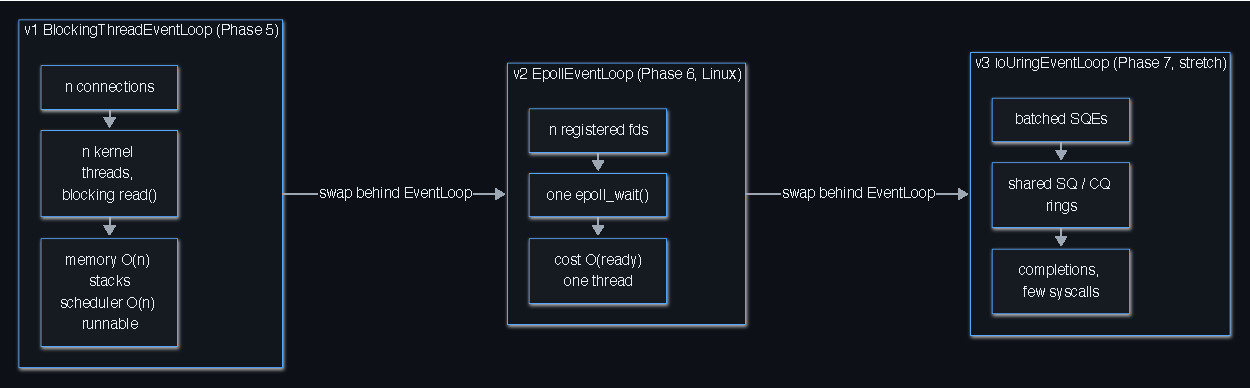
\includegraphics[width=\linewidth]{diagrams/concurrency.pdf}
\caption{The planned v1$\to$v2$\to$v3 progression (Mermaid). Each step replaces one \cc{EventLoop} implementation;
\cc{Server} and \cc{Connection} do not change.}
\label{fig:concprog}
\end{figure}

\begin{figure}[H]
\centering
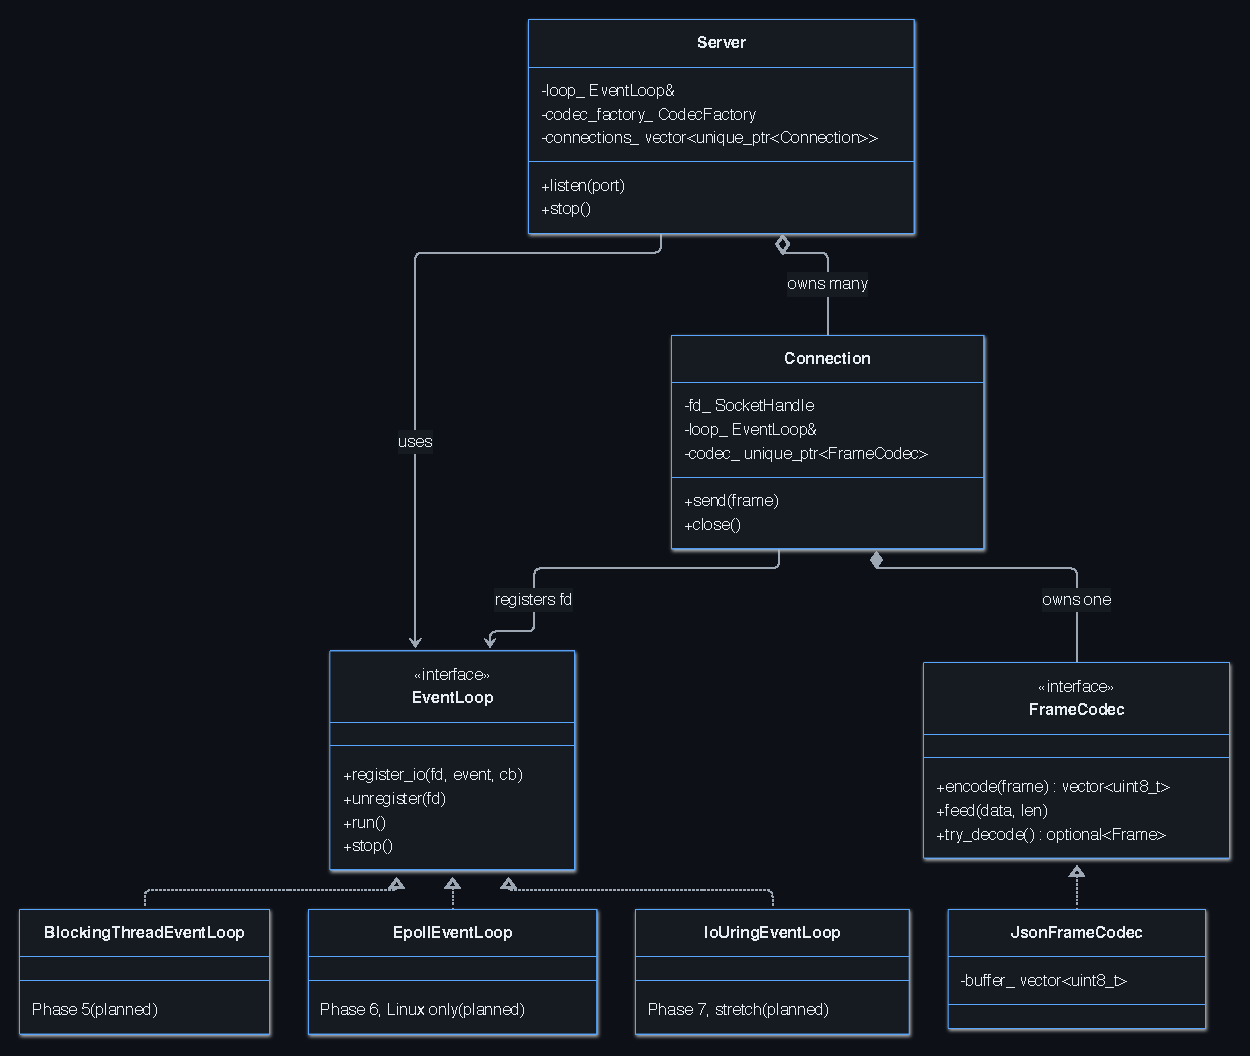
\includegraphics[width=0.8\linewidth]{diagrams/net_classes.pdf}
\caption{\texttt{score::net} class relationships (Mermaid). The three loop implementations are planned (Phases 5--7);
only the interfaces and the \cc{JsonFrameCodec}, \cc{Connection} and \cc{Server} stubs exist today.}
\label{fig:netclasses}
\end{figure}

On macOS there is no \cc{epoll}; the native readiness API is \cc{kqueue}. Decision D4 makes this a matter of adding one
more \cc{EventLoop} implementation rather than a {\ttfamily\color{org}\#ifdef} in \cc{Server}. Phase 4 encodes the same idea in the build:
the \cc{epoll} source is compiled only when CMake reports Linux (\cref{ch:roadmap}).

\begin{exercises}
\ex{ex:pollbudget}{\lvA} Using the fitted slope of \cref{fig:pollbench}, find the $n$ at which a \cc{poll}-based loop
spends half of a 1\,ms tick inside \cc{poll}. Repeat for \cc{kevent} using the measured constant, and explain why the
answer is not a number.

\ex{ex:blocking}{\lvC} \cc{BlockingThreadEventLoop} must implement \cc{register_io(fd, kReadable, cb)}, but a blocking
model has no readiness notification. One design spawns a thread per descriptor that blocks in \cc{recv} and then calls
\cc{cb}. Show that this either loses the bytes it read or requires an interface change, because \cc{IoCallback} carries no
data. Propose the smallest interface change that keeps \cc{Server} unchanged.

\ex{ex:et}{\lvB} Under edge-triggered \cc{epoll}, a handler reads at most 4096 bytes per event and the client has sent
two frames totalling 6000 bytes and then waits for both replies. Prove that the second frame is never decoded. Then
prove that ``read until \cc{EAGAIN}'' removes the deadlock.

\ex{ex:reentrant}{\lvB} A callback invoked by \cc{run()} calls \cc{unregister(fd)} on its own descriptor, or on another
descriptor that is ready in the same batch. Specify semantics for \cc{unregister} that are safe in both cases, and
describe an implementation that never invokes a callback for a descriptor after \cc{unregister} has returned.

\ex{ex:uringadapt}{\lvC} io\_uring can emulate readiness with \cc{IORING_OP_POLL_ADD}. Sketch an
\cc{IoUringEventLoop} that implements the present \cc{EventLoop} interface this way. What does it lose compared with a
true proactor that submits \cc{IORING_OP_RECV}? Would you change the interface instead, and what would that cost the
other two backends?

\ex{ex:memory}{\lvA} Estimate resident memory for $10^4$ idle connections under v1 and v2, assuming 16\,KiB of touched
stack per thread, a 64\,KiB receive buffer in each codec, and 1\,KiB of kernel state per socket. Which term dominates
each model?
\end{exercises}


\chapter{Framing and Codecs: Putting Message Boundaries Back}\label{ch:framing}

\begin{objectives}
\begin{itemize}
\item compare delimiter, length-prefix and self-describing framing;
\item encode a concrete VaR request byte by byte: payload, big-endian prefix, full hex dump;
\item specify the decoder as a state machine and \emph{prove} it reconstructs frames under every segmentation;
\item defend a server against hostile length prefixes;
\item explain what a binary codec changes (fixed-width fields, byte order, varints) and why only the codec changes.
\end{itemize}
{\small\color{muted}\textbf{Chapter references:} Protocol Buffers encoding guide~\cite{protobuf}; nlohmann/json~\cite{nlohmannjson};
Stevens et al.~\cite{stevens2004unp}.}
\end{objectives}

\section{Three ways to mark a boundary}
\Cref{prop:boundary} says TCP will not tell us where messages end, so the bytes must. There are three classic answers.

\begin{center}
\small
\begin{tabularx}{\linewidth}{@{}>{\leavevmode\bfseries\color{yel}}p{2.6cm} X X@{}}
\toprule
\textcolor{muted}{Strategy} & \textcolor{muted}{Mechanism} & \textcolor{muted}{Cost / risk}\\
\midrule
Delimiter & A reserved byte sequence ends each message (newline-delimited JSON; CRLF after HTTP/1.1 header lines). & Payload must escape the delimiter; the decoder scans every byte.\\
Length prefix & A fixed-size header carries the payload length. & Decoder jumps straight to the end; the length is attacker-controlled (\cref{sec:maxframe}).\\
Self-describing & Every field is tagged with its type and length (TLV; Protocol Buffers~\cite{protobuf}). & Most flexible, most complex; still needs an outer frame on a stream.\\
\bottomrule
\end{tabularx}
\end{center}

Decision D5 chose a length prefix: four bytes, unsigned, big-endian, followed by JSON.

\repo[firstline=9,lastline=31]{include/score/net/codec.hpp}{The codec interface. \cc{encode} is pure; \cc{feed} and
\cc{try_decode} split decoding into ``accept bytes'' and ``extract a frame if one is complete'', which is exactly the
shape \cref{thm:segmentation} needs.}{lst:codec}

\repo[firstline=9,lastline=21]{include/score/net/json_codec.hpp}{The v1 codec. Its only state is \cc{buffer_}: the
bytes received but not yet consumed.}{lst:jsoncodec}

\section{Encoding a request, byte by byte}\label{sec:encode}
\begin{definition}[Big-endian unsigned 32-bit integer]
Bytes $b_0b_1b_2b_3$ encode $N=b_0\cdot 2^{24}+b_1\cdot 2^{16}+b_2\cdot 2^{8}+b_3$. Most significant byte first is also
called \emph{network byte order}.
\end{definition}

Take the pre-trade request ``95\% VaR for AAPL'', built as
\begin{center}\cc{nlohmann::json{{"op","var"},{"symbol","AAPL"},{"conf",0.95}}}.\end{center}
We ran it through a reference encoder built
on the repository's own \texttt{nlohmann/json}~3.12.0 submodule (\file{verify/codec_test.cpp}).

\begin{progout}{codec\_test: encoding the request}{lst:encodeout}
dump: {"conf":0.95,"op":"var","symbol":"AAPL"}
len=40 total=44
hex:
  00 00 00 28 7B 22 63 6F 6E 66 22 3A 30 2E 39 35
  2C 22 6F 70 22 3A 22 76 61 72 22 2C 22 73 79 6D
  62 6F 6C 22 3A 22 41 41 50 4C 22 7D
\end{progout}

Three details deserve attention.
\begin{enumerate}[label=\textbf{\color{yel}\arabic*.}]
\item \textbf{Key order changed.} \cc{nlohmann::json}'s default object type is \cc{std::map<std::string, json>},
so \cc{dump()} emits keys \emph{sorted}: \texttt{conf}, \texttt{op}, \texttt{symbol}. Any test that
compares encoded bytes against a hand-written string must account for this.
\item \textbf{Compact output.} \cc{dump()} with no indent emits no spaces or newlines: 40 bytes, so $N=40=\hex{0x28}$
and the prefix is \hex{00 00 00 28}.
\item \textbf{The number is text.} \texttt{0.95} travels as the four ASCII bytes \hex{30 2E 39 35}. The receiver parses
them back to the binary64 value nearest $0.95$, which is $0.9499999999999999555\ldots$ (\cref{ch:float}).
\end{enumerate}

\begin{figure}[htbp]
\centering
\begin{tikzpicture}[x=0.92cm,y=0.95cm]
\def\row#1#2{\foreach \b [count=\i from 0] in {#2}{\node[byte] at (\i,-#1) {\b};}}
\foreach \i/\b in {0/00,1/00,2/00,3/28}{\node[byte,draw=yel,text=yel,fill=yel!12!bg] at (\i,0) {\b};}
\foreach \b [count=\i from 4] in {7B,22,63,6F,6E,66,22,3A,30,2E,39,35}{\node[byte,draw=acc] at (\i,0) {\b};}
\foreach \b [count=\i from 0] in {2C,22,6F,70,22,3A,22,76,61,72,22,2C,22,73,79,6D}{\node[byte,draw=acc] at (\i,-1) {\b};}
\foreach \b [count=\i from 0] in {62,6F,6C,22,3A,22,41,41,50,4C,22,7D}{\node[byte,draw=acc] at (\i,-2) {\b};}
% ascii under
\foreach \c [count=\i from 4] in {\{,",c,o,n,f,",:,0,.,9,5}{\node[font=\scriptsize\ttfamily,text=muted] at (\i,0.55) {\c};}
\foreach \c [count=\i from 0] in {{,},",o,p,",:,",v,a,r,",{,},",s,y,m}{\node[font=\scriptsize\ttfamily,text=muted] at (\i,-0.45) {\c};}
\foreach \c [count=\i from 0] in {b,o,l,",:,",A,A,P,L,",\}}{\node[font=\scriptsize\ttfamily,text=muted] at (\i,-1.45) {\c};}
\foreach \o [count=\r from 0] in {0,16,32}{\node[font=\scriptsize\ttfamily,text=codeframe!50!muted,anchor=east] at (-0.6,-\r) {+\o};}
\draw[decorate,decoration={brace,amplitude=5pt,mirror},draw=yel] (-0.45,-2.5) -- (3.45,-2.5) node[midway,below=6pt,font=\footnotesize,text=yel,align=center]{length prefix\\ $0\cdot2^{24}+0\cdot2^{16}+0\cdot2^{8}+40$};
\draw[decorate,decoration={brace,amplitude=5pt,mirror},draw=acc] (3.55,-2.5) -- (11.45,-2.5) node[midway,below=6pt,font=\footnotesize,text=acc,align=center]{payload: 40 bytes\\ (12 in row +0, 16 in row +16, 12 in row +32)};
\end{tikzpicture}
\caption{The 44-byte frame, 16 bytes per row (TikZ). Yellow: length prefix. Blue: UTF-8 JSON payload, with the ASCII
character above each byte.}
\label{fig:frame}
\end{figure}

\section{The decoder as a state machine}
\begin{figure}[htbp]
\centering
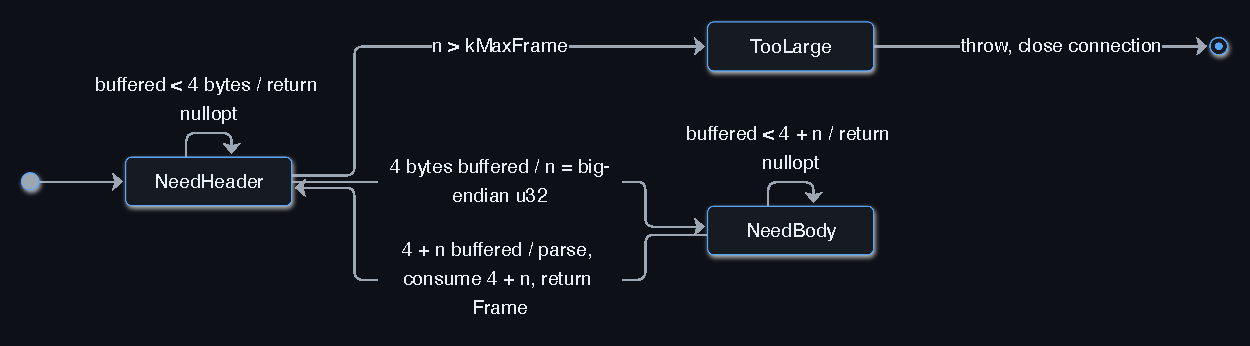
\includegraphics[width=0.92\linewidth]{diagrams/decoder_state.pdf}
\caption{Decoder states (Mermaid). Note that the decoder never needs a separate ``in the middle of a frame'' flag: the
state is a function of the buffered bytes alone.}
\label{fig:decoderstate}
\end{figure}

\Cref{lst:sketch} is a reference implementation, written for this tutorial and \emph{not} part of the repository, whose
\cc{JsonFrameCodec} still throws (\cref{lst:jsonstub}). It differs from the repository's header only in carrying a read
offset \cc{pos_} so that consuming a frame does not shift the buffer (\cref{ex:quadratic}).

\begin{code}{codec\_sketch.hpp: a reference length-prefixed JSON codec}{lst:sketch}
class SketchJsonFrameCodec {
public:
    static constexpr std::uint32_t kMaxFrame = 1u << 20;  // 1 MiB

    std::vector<std::uint8_t> encode(const Frame& f) const {
        const std::string body = f.payload.dump();
        const auto n = static_cast<std::uint32_t>(body.size());
        std::vector<std::uint8_t> out{
            static_cast<std::uint8_t>(n >> 24), static_cast<std::uint8_t>(n >> 16),
            static_cast<std::uint8_t>(n >> 8),  static_cast<std::uint8_t>(n)};
        out.insert(out.end(), body.begin(), body.end());
        return out;
    }

    void feed(const std::uint8_t* data, std::size_t len) {
        buf_.insert(buf_.end(), data, data + len);
    }

    std::optional<Frame> try_decode() {
        if (buf_.size() - pos_ < 4) return std::nullopt;            // HEADER: need 4 bytes
        const std::uint8_t* p = buf_.data() + pos_;
        const std::uint32_t n = (std::uint32_t{p[0]} << 24) | (std::uint32_t{p[1]} << 16) |
                                (std::uint32_t{p[2]} << 8)  |  std::uint32_t{p[3]};
        if (n > kMaxFrame) throw std::length_error("frame too large");
        if (buf_.size() - pos_ - 4 < n) return std::nullopt;        // BODY: need n bytes
        Frame f{nlohmann::json::parse(p + 4, p + 4 + n)};
        pos_ += 4 + n;
        if (pos_ == buf_.size()) { buf_.clear(); pos_ = 0; }        // compact when drained
        return f;
    }

private:
    std::vector<std::uint8_t> buf_;
    std::size_t pos_ = 0;
};
\end{code}

\section{Correctness under arbitrary segmentation}
\begin{theorem}[Segmentation invariance]\label{thm:segmentation}
Let $f_1,\dots,f_m$ be frames whose encodings $e_j=\mathrm{enc}(f_j)$ satisfy $|e_j|-4\le$ \cc{kMaxFrame}, and let
$S=e_1\Vert\cdots\Vert e_m$. Partition $S$ into consecutive chunks $c_1,\dots,c_q$ (any $q\ge1$, any lengths, empty chunks
allowed). Run, for $i=1,\dots,q$: \cc{feed}$(c_i)$, then call \cc{try_decode} until it returns \cc{nullopt}. Then the
frames returned, in order, are exactly $f_1,\dots,f_m$, and afterwards the buffer is empty.
\end{theorem}

\begin{proof}
Let $E_j=|e_1|+\cdots+|e_j|$ (so $E_0=0$), let $F$ be the number of bytes fed so far, and let $d$ be the number of frames
returned so far. We claim the following invariant holds between calls:

\smallskip
\textbf{(I)} the unconsumed bytes \cc{buf_[pos_..)} equal $S[E_d, F)$, and the frames returned are $f_1,\dots,f_d$.

\smallskip
\emph{Initially} $d=F=0$ and the buffer is empty, so (I) holds. \emph{\cc{feed}} appends $c_i$, which is $S[F,F+|c_i|)$
because chunks are consecutive, and leaves $d$ unchanged; (I) holds with the new $F$. \emph{\cc{try_decode}}: let
$U=S[E_d,F)$ be the unconsumed bytes. If $|U|<4$ it returns \cc{nullopt} and changes nothing. Otherwise, by (I), the
first four bytes of $U$ are the first four bytes of $e_{d+1}$, that is, the prefix of $f_{d+1}$, so the decoded $n$ is
$|e_{d+1}|-4\le$ \cc{kMaxFrame} and no exception is thrown. If $|U|<4+n$ it returns \cc{nullopt}. Otherwise
$U[4,4+n)$ is exactly the payload of $f_{d+1}$, so it returns $f_{d+1}$ and advances \cc{pos_} by $4+n=|e_{d+1}|$;
the unconsumed bytes become $S[E_{d+1},F)$ and (I) holds with $d+1$. The compaction branch only discards
already-consumed bytes and preserves (I).

\emph{Termination}: each successful call consumes at least 4 bytes, so each inner loop ends. \emph{Completeness}: after
the last chunk, $F=|S|=E_m$. If $d<m$ then $U=S[E_d,E_m)$ begins with the whole of $e_{d+1}$, so the next call succeeds.
The loop therefore stops only when $d=m$, at which point $U$ is empty.
\end{proof}

\begin{remarkbox}
The proof uses one property of the decoder: its decision depends only on the bytes buffered so far, and more bytes
never turn a ``complete'' answer into ``incomplete''. Any framing with that \emph{prefix-monotone} property, such as
newline delimiting with escaped payloads, admits the same proof.
\end{remarkbox}

\begin{verified}
\file{verify/codec_test.cpp} concatenates the request with a second frame,
\texttt{\{"conf":0.975,"op":"cvar","symbol":"MSFT"\}} (42-byte payload), into a 90-byte stream and checks
\emph{every} split into three consecutive chunks, i.e.\ every pair $0\le i\le j\le 90$:
$\binom{92}{2}=4186$ cases, all decoding to the two original frames. Feeding one byte at a time also yields exactly two
frames.
\end{verified}

\begin{example}[One frame across three reads]\label[example]{ex:threereads}
Suppose the 44 bytes of \cref{fig:frame} arrive as reads of 3, 20 and 21 bytes, as they did on loopback in
\cref{lst:streamout}. The decoder's view:
\begin{center}
\small
\begin{tabular}{@{}clrll@{}}
\toprule
\textcolor{muted}{read} & \textcolor{muted}{bytes received} & \textcolor{muted}{buffered} & \textcolor{muted}{state} & \textcolor{muted}{\cc{try_decode}}\\
\midrule
1 & \hex{00 00 00} & 3 & need header ($3<4$) & \cc{nullopt}\\
2 & \hex{28 7B 22 \dots\ 22 3A 22} & 23 & header read, $n=40$; need $44$ & \cc{nullopt}\\
3 & \hex{76 61 72 \dots\ 4C 22 7D} & 44 & complete & frame; buffer cleared\\
\bottomrule
\end{tabular}
\end{center}
Notice that the length prefix itself was split: read 1 delivered three of its four bytes. A decoder that read the length
from ``the first four bytes of this read'' would have computed $\hex{0x00000028}$ only by luck in some runs and garbage in
others. The run of \file{verify/codec_test.cpp} printed \texttt{nullopt}, \texttt{nullopt}, and the decoded object for the
three reads, in agreement with the table.
\end{example}

\begin{figure}[htbp]
\centering
\begin{tikzpicture}[x=0.3cm,y=0.9cm]
\foreach \i in {0,...,3}{\draw[draw=yel,fill=codebg] (\i,0) rectangle ++(1,0.7);}
\foreach \i in {4,...,43}{\draw[draw=acc,fill=codebg] (\i,0) rectangle ++(1,0.7);}
\fill[yel!35!codebg] (0.05,0.05) rectangle (3.95,0.65);
\draw[very thick,red] (3,-0.25) -- (3,0.95);
\draw[very thick,red] (23,-0.25) -- (23,0.95);
\node[font=\footnotesize,text=fg] at (1.5,1.35) {read 1};
\node[font=\footnotesize,text=fg] at (13,1.35) {read 2: 20 bytes};
\node[font=\footnotesize,text=fg] at (33.5,1.35) {read 3: 21 bytes};
\node[font=\scriptsize,text=yel,anchor=north] at (2,-0.3) {prefix};
\node[font=\scriptsize,text=red,anchor=north] at (13,-0.3) {cuts at byte 3 and byte 23};
\node[font=\scriptsize,text=muted,anchor=north] at (36,-0.3) {payload ends at byte 44};
\end{tikzpicture}
\caption{The split of \cref{ex:threereads} (TikZ). The first cut falls inside the length prefix.}
\label{fig:threereads}
\end{figure}

\section{Defending against hostile lengths}\label{sec:maxframe}
The length prefix is chosen by whoever is on the other end of the socket. Without a bound, the four bytes
\hex{FF FF FF FF} announce a $4{,}294{,}967{,}295$-byte payload, almost exactly 4\,GiB.

\begin{pitfall}[title={Pitfall: trusting the prefix}]
A decoder that does \cc{buffer.reserve(n)} as soon as it reads $n$ lets one 4-byte message from any client allocate
4\,GiB. A decoder that merely waits for $n$ bytes lets a client grow the buffer without limit by sending slowly. Both are
denial-of-service bugs.
\end{pitfall}

\begin{proposition}[Per-connection memory bound]\label[proposition]{prop:membound}
With the check \cc{n > kMaxFrame} in place, and reads of at most $R$ bytes fed only while \cc{try_decode} has been
drained, a connection's buffered bytes never exceed $4+\text{\cc{kMaxFrame}}+R$.
\end{proposition}
\begin{proof}
After draining, the unconsumed bytes are a proper prefix of one frame (else another frame would decode), so they number at
most $4+n-1\le 3+\text{\cc{kMaxFrame}}$, or the header check has thrown. One more read adds at most $R$.
\end{proof}

The bound covers memory, not time: a client can hold a partial frame open forever and tie up a descriptor. That needs an
idle timeout, which belongs to \cc{Connection}, not to the codec. The verification program also checked that the prefix
\hex{7F FF FF FF} ($2{,}147{,}483{,}647$) makes \cc{try_decode} throw \cc{std::length_error} before any allocation.

\section{Toward a binary codec}
JSON spends bytes on punctuation and field names and turns every number into decimal text. A binary codec (Phase 8)
replaces this with fixed-width fields and explicit byte order, and optionally \emph{varints}.

\begin{definition}[Base-128 varint]\label[definition]{def:varint}
An unsigned integer is written in 7-bit groups, least significant group first; every byte except the last has its high
bit set. Protocol Buffers uses this encoding, mapping signed integers through the zig-zag transform
$z(v)=2v$ for $v\ge0$ and $z(v)=-2v-1$ for $v<0$ so that small negative numbers stay short~\cite{protobuf}.
\end{definition}

\begin{verified}
Encodings computed by \file{verify/encodings.py}: $40\mapsto$ \hex{28}; $127\mapsto$ \hex{7F};
$128\mapsto$ \hex{80 01}; $300\mapsto$ \hex{AC 02}; $9500\mapsto$ \hex{9C 4A}. Zig-zag: $-1\mapsto1$, $1\mapsto2$.
As a fixed-width big-endian \texttt{u16}, $9500$ is \hex{25 1C} and $9750$ is \hex{26 16}.
\end{verified}

A binary layout for the same request could be: one byte of opcode, one byte of symbol length, the symbol's ASCII bytes,
and the confidence as a \texttt{u16} in basis points:
\hex{01}\,\textbar\,\hex{04}\,\textbar\,\hex{41 41 50 4C}\,\textbar\,\hex{25 1C}: 8 payload bytes instead of 40, and, as
\cref{ch:float} will show, a confidence that is an exact integer instead of an inexact binary fraction.

\repo[firstline=13,lastline=22]{include/score/net/server.hpp}{\cc{CodecFactory} is why only the codec changes: \cc{Server}
asks the factory for one codec per connection and never names a concrete codec type. Switching to binary means passing a
different lambda at the call site that constructs \cc{Server}.}{lst:codecfactory}

\begin{exercises}
\ex{ex:cvarframe}{\lvA} Encode \texttt{\{"op":"cvar","symbol":"MSFT","conf":0.975\}} by hand, remembering that
\cc{dump()} sorts keys. Give the payload length, the four prefix bytes, and the first eight payload bytes in hex.

\ex{ex:quadratic}{\lvB} The repository's \cc{JsonFrameCodec} holds only \cc{std::vector<std::uint8_t> buffer_}. If each
decoded frame is removed with \cc{buffer_.erase(begin, begin + 4 + n)}, show that one read containing $k$ small frames
costs $\Theta(k^2)$ byte moves. Prove that the \cc{pos_} offset with compaction-on-drain in \cref{lst:sketch} is $O(k)$,
and find the input pattern for which it never compacts.

\ex{ex:ndjson}{\lvB} Prove that newline-delimited JSON is segmentation-invariant if and only if no payload contains a raw
\hex{0A} byte, and argue from the JSON grammar that compact \cc{dump()} never emits one.

\ex{ex:maxframe}{\lvB} Choose \cc{kMaxFrame} from first principles. A backtest reply carries $N$ bars of six fields as
JSON. Estimate bytes per bar from \cref{fig:frame}'s density, find the largest $N$ under 1\,MiB, and decide whether
replies should instead be streamed as many frames.

\ex{ex:binary}{\lvC} Design the Phase 8 binary frame: magic, version, message type, request id, body. Show how a v2 server
can accept v1 clients, and prove that your header can be parsed with the same prefix-monotone decoder as
\cref{thm:segmentation}.

\ex{ex:badjson}{\lvB} A complete frame contains malformed JSON. Should \cc{try_decode} throw, return an error frame, or
close the connection? Consider that it is called from inside an \cc{IoCallback} running on the loop thread.
\end{exercises}


\chapter{Columnar Storage for Daily Bars}\label{ch:columnar}

\begin{objectives}
\begin{itemize}
\item describe row and column layouts of \cc{score::db::Bar} down to byte offsets measured on a real compiler;
\item derive how many bytes and cache lines a close-to-close return computation touches in each layout;
\item prove that a sorted, append-only date column answers \cc{scan(start, end)} in $O(\log n+k)$;
\item prove that ISO-8601 date strings sort chronologically, and say what the interface fails to enforce;
\item recognise \cc{IngestionSource} as the Strategy pattern and connect both data paths to it.
\end{itemize}
{\small\color{muted}\textbf{Chapter references:} Copeland and Khoshafian~\cite{copeland1985dsm}; Stonebraker et al.~\cite{stonebraker2005cstore};
Boncz et al.~\cite{boncz2005x100}; Abadi et al.~\cite{abadi2008colrow,abadi2013design}; Gamma et al.~\cite{gamma1994design};
Glasserman~\cite{glasserman2003monte}; Kx~\cite{kxq}.}
\end{objectives}

\section{The workload decides the layout}
Decision D8 named the two consumers: pre-trade risk checks and backtests. Both ask the same question, ``give me the closes
of \emph{one} symbol between two dates'', and then run arithmetic down that sequence (\cref{ch:risk}). Neither ever asks
for ``all fields of one bar''. That asymmetry is the whole case for a column store.

\repo[firstline=8,lastline=16]{include/score/db/bar.hpp}{One daily OHLCV row. The date is a \cc{std::string} holding
\texttt{"YYYY-MM-DD"}.}{lst:bar}

\repo[firstline=10,lastline=30]{include/score/db/column_store.hpp}{The storage contract. It commits to append and
range-scan semantics but deliberately not to a byte layout; \cc{ColumnStoreV1} currently throws from every method.}{lst:colstore}

\begin{definition}[Row store, column store~\cite{copeland1985dsm}]\label[definition]{def:rowcol}
For a relation with attributes $A_1,\dots,A_d$ and tuples $t_1,\dots,t_n$, a \emph{row layout} stores
$t_1[A_1],\dots,t_1[A_d],t_2[A_1],\dots$ contiguously; a \emph{column layout} stores, for each attribute separately,
$t_1[A_j],t_2[A_j],\dots,t_n[A_j]$ contiguously. Copeland and Khoshafian called the fully decomposed form the
Decomposition Storage Model.
\end{definition}

\section{The bytes, measured}
On the measurement machine (Apple clang 21, libc++, arm64) we compiled \cc{Bar} and printed its layout.

\begin{progout}{layout.cpp: sizeof and offsetof for score::db::Bar}{lst:layoutout}
sizeof(std::string)=24 sizeof(Bar)=64 alignof(Bar)=8
offsets: date=0 open=24 high=32 low=40 close=48 volume=56
PackedRow sizeof=48 offsets date=0 open=8 close=32 volume=40
SSO: string data inside object? 1 (capacity 22)
\end{progout}

The 10-character date fits libc++'s short-string buffer (capacity 22), so it lives inside the 24-byte \cc{std::string}
object and \cc{Bar} is exactly one 64-byte cache line. \cc{PackedRow}, a hypothetical on-disk row with the date as
\cc{int32} days, still occupies 48 bytes because the following \cc{double} must be 8-aligned.

\begin{figure}[htbp]
\centering
\begin{tikzpicture}[x=0.17cm,y=0.75cm]
  \node[font=\small\bfseries,text=fg,anchor=west] at (0,1.2) {Row layout: \texttt{std::vector<Bar>}, 64 bytes per bar};
  \foreach \r in {0,1,2}{
    \pgfmathtruncatemacro{\y}{-\r}
    \draw[draw=muted,fill=codebg] (0,\y) rectangle (24,\y+0.75); \node[font=\scriptsize\ttfamily,text=muted] at (12,\y+0.37) {date (24)};
    \foreach \x/\l in {24/open,32/high,40/low}{\draw[draw=muted,fill=codebg] (\x,\y) rectangle ++(8,0.75); \node[font=\scriptsize\ttfamily,text=muted] at (\x+4,\y+0.37) {\l};}
    \draw[draw=red,fill=red!30!bg,thick] (48,\y) rectangle ++(8,0.75); \node[font=\scriptsize\ttfamily,text=fg] at (52,\y+0.37) {close};
    \draw[draw=muted,fill=codebg] (56,\y) rectangle ++(8,0.75); \node[font=\scriptsize\ttfamily,text=muted] at (60,\y+0.37) {vol};
    \node[font=\scriptsize,text=muted,anchor=east] at (-0.5,\y+0.37) {bar \r};
  }
  \node[font=\scriptsize,text=red,anchor=west] at (65,-0.63) {8 useful bytes per 64-byte line};
  \foreach \x in {0,16,32,48,64}{\node[font=\tiny\ttfamily,text=muted] at (\x,-2.35) {\x};}
  % columns
  \node[font=\small\bfseries,text=fg,anchor=west] at (0,-3.4) {Column layout: one array per field};
  \foreach \i in {0,...,7}{\draw[draw=grn,fill=grn!30!bg,thick] (\i*8,-4.6) rectangle ++(8,0.75); \node[font=\scriptsize\ttfamily,text=fg] at (\i*8+4,-4.23) {c\textsubscript{\i}};}
  \node[font=\scriptsize,text=muted,anchor=east] at (-0.5,-4.23) {close};
  \node[font=\scriptsize,text=grn,anchor=west] at (65,-4.23) {8 closes per 64-byte line};
  \foreach \i in {0,...,7}{\draw[draw=muted,fill=codebg] (\i*8,-5.6) rectangle ++(8,0.75); \node[font=\scriptsize\ttfamily,text=muted] at (\i*8+4,-5.23) {o\textsubscript{\i}};}
  \node[font=\scriptsize,text=muted,anchor=east] at (-0.5,-5.23) {open};
  \node[font=\scriptsize,text=muted,anchor=west] at (65,-5.23) {not read by the query};
\end{tikzpicture}
\caption{Byte-level picture of the two layouts, using the offsets of \cref{lst:layoutout} (TikZ). Red: the close fields a
return computation needs, scattered one per cache line. Green: the same values packed eight per line.}
\label{fig:rowcol}
\end{figure}

\begin{proposition}[Bytes touched by a close-to-close scan]\label[proposition]{prop:bytes}
Let a scan read the close of $k$ consecutive bars, let the row width be $w$ bytes with the close field $f$ bytes wide,
and let cache lines be $L$ bytes with $w\ge L$ and $w$ a multiple of $L$. Then the row layout brings at least
$k$ lines, $kL$ bytes, into cache, while the column layout brings $\lceil kf/L\rceil+1$ lines at most. For $w=L=64$,
$f=8$ the ratio approaches $8$.
\end{proposition}
\begin{proof}
In the row layout the $k$ close fields sit at stride $w\ge L$, so no two of them share a line, and each needs its own line.
In the column layout they occupy $kf$ contiguous bytes, which span at most $\lceil kf/L\rceil+1$ lines (the $+1$ accounts
for a misaligned start). The ratio $kL/(\lceil kf/L\rceil+1)\to L^2/(fL)=L/f=8$.
\end{proof}

\begin{verified}
For the mock generator's $n=504$ bars: row layout $504\times64=32{,}256$ bytes in 504 lines; packed on-disk rows
$504\times48=24{,}192$ bytes; close column $504\times8=4{,}032$ bytes in 63 lines (aligned). Ten years of 252 trading
days for 500 symbols multiplies each by 2500.
\end{verified}

Bytes are only the first advantage. A column of closes is a dense \cc{double} array, which a compiler can vectorise and
a codec can compress (dates are an arithmetic progression with weekend gaps; volumes vary slowly in magnitude).
C-Store~\cite{stonebraker2005cstore} and MonetDB/X100~\cite{boncz2005x100} built whole systems on these
observations; Abadi, Madden and Hachem measured why simply storing rows by column inside a row engine does not capture
the benefit~\cite{abadi2008colrow}; and the survey by Abadi et al.\ covers the design space~\cite{abadi2013design}.

\begin{history}
Column orientation is old. Copeland and Khoshafian's Decomposition Storage Model appeared at SIGMOD in
1985~\cite{copeland1985dsm}. In finance, Kx Systems' kdb+ and its q language have long stored tick data column-wise
for exactly the ``one symbol, one time range, one field'' queries a risk engine issues~\cite{kxq}.
\end{history}

\section{Sorted, append-only columns}
\begin{lemma}[ISO-8601 dates sort chronologically]\label[lemma]{lem:iso}
For valid dates written as zero-padded \texttt{YYYY-MM-DD} strings with four-digit years, lexicographic comparison of
the strings agrees with chronological order.
\end{lemma}
\begin{proof}
All such strings have length 10, with \texttt{-} at positions 4 and 7, so lexicographic order compares
the digits position by position. For fixed-width zero-padded decimal numerals, digit-wise lexicographic order is numeric
order. The fields appear in order of significance (year, month, day), so the string order is the lexicographic order
of the triple $(Y,M,D)$, which is chronological order.
\end{proof}

\begin{pitfall}[title={Pitfall: the lemma has hypotheses}]
\texttt{"2024-5-7"} $>$ \texttt{"2024-05-07"} lexicographically, because \texttt{'5'} $>$ \texttt{'0'}. The interface types the
date as \cc{std::string}, so nothing stops such a value. \cc{append} must validate the format, or the store must keep
dates as integers (\cref{ex:intdate}).
\end{pitfall}

\begin{theorem}[Range scan]\label{thm:scan}
Suppose the date column of a symbol holds $n$ dates $d_1<d_2<\dots<d_n$ (strictly increasing). Then the indices of all
bars with $d_i\in[s,e]$ form a contiguous range $[\ell, u)$ found with $2\lceil\log_2(n+1)\rceil$ comparisons, and
\cc{scan(symbol, s, e)} costs $O(\log n + k)$ where $k=u-\ell$ is the number of bars returned.
\end{theorem}
\begin{proof}
Let $\ell=\min\{i: d_i\ge s\}$ (lower bound) and $u=\min\{i: d_i> e\}$ (upper bound), with the convention $n+1$ if no
such index exists. Because the column is sorted, $d_i\in[s,e]\iff \ell\le i<u$: for $i<\ell$, $d_i<s$; for $i\ge u$,
$d_i>e$; between them, $s\le d_\ell\le d_i\le d_{u-1}\le e$. Each bound is a binary search over $n+1$ candidate
positions, needing $\lceil\log_2(n+1)\rceil$ comparisons. Copying the $k$ bars costs $O(k)$ per column read.
\end{proof}

For $n=504$, $\lceil\log_2 505\rceil=9$ comparisons per bound. The strictness hypothesis is what the interface comment
asks of \cc{append}: reject bars ``out of order or overlap[ping] dates already stored''.

\begin{proposition}[Append preserves sortedness]\label[proposition]{prop:append}
If the stored column is strictly increasing, and an appended batch $b_1<\dots<b_m$ satisfies $b_1>d_n$, the result is
strictly increasing. The check costs $O(m)$ and needs only the last stored date.
\end{proposition}
\begin{proof}
The concatenation is increasing within each part and across the seam, since $d_n<b_1$. Checking means one comparison
with $d_n$ and $m-1$ adjacent comparisons within the batch.
\end{proof}

\section{IngestionSource as a Strategy}\label{sec:gbm}
\repo[firstline=9,lastline=25]{include/score/db/ingestion.hpp}{One interface for any producer of bars. The comment names
both Python paths as future implementations.}{lst:ingestion}

\begin{layman}
A kitchen does not care whether the vegetables came from the market this morning or from the freezer; it cares that they
arrive washed, cut, and labelled the same way. \cc{IngestionSource} is the loading dock: live \cc{yfinance} data and
synthetic GBM data unload through the same door, so the store and the risk code never learn which truck brought them.
\end{layman}

In the vocabulary of Gamma et al.~\cite{gamma1994design}, \cc{IngestionSource} is a \emph{Strategy}: a family of
interchangeable algorithms (``where do bars come from?'') behind one interface, chosen by the caller at run time. The
context object is whatever calls \cc{ingest(store, symbol)}; the \cc{ColumnStore} it receives is itself an abstraction,
so the two hierarchies vary independently (\cref{fig:ingest}).

\begin{figure}[htbp]
\centering
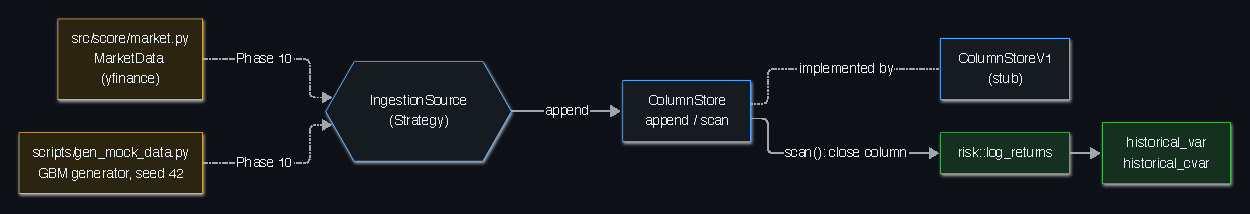
\includegraphics[width=\linewidth]{diagrams/ingestion.pdf}
\caption{Data flow after Phase 10 (Mermaid). Yellow: Python producers, today disconnected. Dotted: bridges that do not
exist yet. Green: the risk code that already works.}
\label{fig:ingest}
\end{figure}

\subsection{The synthetic path, exactly}
\Cref{lst:gbm} implements the solution of the GBM stochastic differential equation $dS=\mu S\,dt+\sigma S\,dW$. By
It\^o's lemma, $\ln S$ is a Brownian motion with drift $\mu-\frac12\sigma^2$ and volatility $\sigma$, so
\[ \ln S_{t+\Delta t}-\ln S_t \sim \mathcal N\!\big((\mu-\tfrac12\sigma^2)\Delta t,\ \sigma^2\Delta t\big) \]
exactly, with independent increments. Simulating in log space therefore has \emph{no discretisation error}, unlike an Euler
step $S_{t+\Delta t}=S_t(1+\mu\Delta t+\sigma\sqrt{\Delta t}Z)$~\cite{glasserman2003monte}. Two details of the code are worth
noticing. First, \cc{np.concatenate(([0.0], np.cumsum(log_increments[:-1])))} uses $N-1$ of the $N$ increments, so the
last normal draw is generated and discarded; the path still has $N$ prices, the first equal to the initial price.
Second, the daily log-returns of the generated closes have model standard deviation $\sigma\sqrt{\Delta t}$, which for
AAPL's $\sigma=0.28$ is $0.28/\sqrt{252}=0.017638$; the realised sample standard deviation of the 503 returns,
computed by the repository's \cc{risk::calculate_risk_from_returns}, is $0.017694$ (\cref{sec:mockvar}).

\begin{exercises}
\ex{ex:ondisk}{\lvC} Design \cc{ColumnStoreV1}'s on-disk layout: one file per (symbol, column), a header with magic,
version, element type and count, then raw little-endian values. Specify the write order (data, \cc{fsync}, header count,
\cc{fsync}) that makes \cc{append} crash-safe, and prove that a crash at any point leaves a store that \cc{scan} reads as
either the old or the new contents.

\ex{ex:bytes500}{\lvA} A nightly batch computes 97.5\% CVaR over 10 years of daily closes for 500 symbols. Compute bytes
read from memory in each layout using \cref{prop:bytes}, and the time at 20\,GB/s of memory bandwidth.

\ex{ex:intdate}{\lvB} Replace the \cc{std::string} date with \cc{int32_t} days since 1970-01-01. Prove that the map from
valid Gregorian dates to day numbers is strictly increasing, give the size of \cc{Bar} after the change (predict, then
check with \cc{sizeof}), and list every place the string form must still exist.

\ex{ex:scanedge}{\lvA} Specify \cc{scan} for: an unknown symbol; $s>e$; $s$ and $e$ both between two stored dates;
malformed date strings. Which should throw \cc{score::DomainError}, and which should return an empty vector? Justify each
from the users named in D8.

\ex{ex:yf}{\lvA} \cc{MarketData} (\cref{lst:market}) fetches \cc{history(period="1d")}. How many log-returns can a
historical VaR compute from that, and what does \cc{historical_var} do with them at $c=0.95$? Specify what a
\cc{YFinanceSource::ingest} must request instead, and how it should avoid re-appending dates already stored.

\ex{ex:compress}{\lvB} Store closes as integer ticks of \$0.0001 (the mock generator rounds to four decimals). Estimate,
from the GBM model, the typical absolute day-to-day change in ticks for AAPL, and hence the bits per value of a
delta-plus-varint encoding (\cref{def:varint}). Compare with 64 bits per \cc{double}.
\end{exercises}


\chapter{Risk Mathematics: Value at Risk and Expected Shortfall}\label{ch:risk}

\begin{objectives}
\begin{itemize}
\item define log-returns, Value at Risk and Expected Shortfall precisely, with sign conventions stated;
\item read the repository's historical-simulation estimator line by line and write it as order statistics;
\item place it among the Hyndman--Fan sample-quantile definitions and prove the inequalities between them;
\item work the ten-point example at $c\in\{0.95,0.90,0.80\}$ and the 503-return AAPL mock series;
\item state the coherence axioms, verify that VaR violates subadditivity, and prove that ES satisfies it;
\item explain why Basel's FRTB moved from 99\% VaR to 97.5\% ES.
\end{itemize}
{\small\color{muted}\textbf{Chapter references:} Artzner et al.~\cite{artzner1999coherent}; Acerbi and Tasche~\cite{acerbi2002coherence};
Rockafellar and Uryasev~\cite{rockafellar2000cvar,rockafellar2002general}; Hyndman and Fan~\cite{hyndman1996sample};
McNeil, Frey and Embrechts~\cite{mcneil2015qrm}; Jorion~\cite{jorion2007var}; Kupiec~\cite{kupiec1995techniques};
BCBS~\cite{bcbs1996amendment,bcbs2019frtb}.}
\end{objectives}

\section{Log-returns}
\begin{definition}[Log-return]\label[definition]{def:logret}
For positive prices $P_0,\dots,P_n$, the log-returns are $r_t=\ln(P_t/P_{t-1})$, $t=1,\dots,n$.
\end{definition}
Log-returns add over time: $\sum_{t=a+1}^{b}r_t=\ln(P_b/P_a)$. A log-return $r$ corresponds to the simple return
$e^r-1$, so a log-return of $-0.05$ is a loss of $1-e^{-0.05}=4.88\%$ of value. The repository computes VaR on
whatever series it is given; when that series is log-returns, the reported number is a loss in log units.

\repo[firstline=50,lastline=72]{src/statistics/risk.cpp}{\cc{risk::log_returns}. Every price must be positive (the
logarithm requires it), and $n+1$ prices yield $n$ returns.}{lst:logret}

\section{Value at Risk}
\begin{definition}[Value at Risk]\label[definition]{def:var}
Let $X$ be a return (profit positive, loss negative) with distribution function $F_X$, and let $c\in(0,1)$ be the
confidence level. The Value at Risk at level $c$ is
\[ \VaR_c(X) \;=\; -\inf\{x\in\R : F_X(x) > 1-c\}. \]
\end{definition}

\begin{layman}
Line up a thousand past trading days from worst to best. The 95\% VaR is roughly ``how bad the 50th-worst day was''.
It says nothing about how bad the 49 days beyond it were, and that blind spot is the subject of \cref{sec:es}.
\end{layman}

\begin{lemma}[Agreement with the loss convention]\label[lemma]{lem:lossconv}
With $L=-X$, \cref{def:var} equals $\inf\{\ell: \Prob(L>\ell)\le 1-c\}$, the loss-based definition of
McNeil, Frey and Embrechts~\cite{mcneil2015qrm}.
\end{lemma}
\begin{proof}
$\Prob(L>\ell)=\Prob(X<-\ell)$. Put $x=-\ell$: the condition $\Prob(X<x)\le 1-c$ holds exactly for $x\le q^+$, where
$q^+=\inf\{x:F_X(x)>1-c\}$ is the upper $(1-c)$-quantile (for $x<q^+$, $F_X(x)\le 1-c$; at $x=q^+$,
$\Prob(X<q^+)=\lim_{y\uparrow q^+}F_X(y)\le1-c$; for $x>q^+$, $\Prob(X<x)\ge F_X(y)>1-c$ for some $y\in(q^+,x)$). So the
set of admissible $\ell$ is $[-q^+,\infty)$ and its infimum is $-q^+=\VaR_c(X)$.
\end{proof}

\section{The repository's estimator}
\repo[firstline=13,lastline=48]{src/statistics/risk.cpp}{The shared helper. The tail size is
$k=\lfloor(1-c)\,n+10^{-9}\rfloor$; the epsilon is the subject of \cref{ch:float}. The comment states the post-condition:
the tail is \cc{sorted_returns[0, tail_index)}, its last element is the VaR order statistic, and its mean is CVaR.}{lst:tail}

\repo[firstline=102,lastline=111]{src/statistics/risk.cpp}{The two estimators. Both clamp at zero, so a sample whose worst
$k$ returns are all gains reports zero risk rather than a negative number.}{lst:varcvar}

\begin{definition}[Repository historical-simulation estimators]\label[definition]{def:repoest}
Given returns $X_1,\dots,X_n$ with order statistics $\ord1\le\dots\le\ord n$, confidence $c$, and
$k=\lfloor(1-c)n+\varepsilon\rfloor$ with $\varepsilon=10^{-9}$: if $k=0$ the estimators throw \cc{score::DomainError};
otherwise
\[ \widehat{\VaR}{}^{\,\mathrm{repo}}_c=\max\bigl(0,-\ord{k}\bigr),\qquad
   \widehat{\CVaR}{}^{\,\mathrm{repo}}_c=\max\Bigl(0,-\tfrac1k\textstyle\sum_{i=1}^{k}\ord{i}\Bigr). \]
\end{definition}

\section{Order statistics and the quantile zoo}
Plugging the empirical distribution $F_n$ into \cref{def:var} is the natural ``historical simulation'', but it is not what the
code computes, and it is worth knowing exactly how they differ. Hyndman and Fan catalogued nine sample-quantile
definitions in use in statistical packages~\cite{hyndman1996sample}; their \emph{type 1} is the inverse of the empirical
CDF. NumPy exposes it as \cc{method="inverted_cdf"}.

\begin{proposition}[Three empirical VaRs]\label[proposition]{prop:threevar}
Let $p=1-c$ and suppose $\varepsilon$ does not change $\lfloor pn\rfloor$ (\cref{thm:epsfloor}). Then, ignoring the clamp:
\begin{enumerate}[label=(\alph*)]
\item the plug-in of \cref{def:var} is $-\ord{\lfloor pn\rfloor+1}$;
\item the type-1 (lower) quantile $\inf\{x: F_n(x)\ge p\}$ gives $-\ord{\lceil pn\rceil}$;
\item the repository gives $-\ord{\lfloor pn\rfloor}$ (defined when $\lfloor pn\rfloor\ge1$).
\end{enumerate}
Hence $\widehat\VaR{}^{\mathrm{repo}}\ge\widehat\VaR{}^{\mathrm{type\,1}}\ge\widehat\VaR{}^{\mathrm{plug\text{-}in}}$, with
the first equality whenever $pn$ is an integer and the second whenever it is not.
\end{proposition}
\begin{proof}
$F_n(x)=j/n$ for $\ord j\le x<\ord{j+1}$ (ties only merge steps). (a) $F_n(x)>p\iff \#\{i:X_i\le x\}>pn\iff
\#\{\cdot\}\ge\lfloor pn\rfloor+1\iff x\ge\ord{\lfloor pn\rfloor+1}$, so the infimum is $\ord{\lfloor pn\rfloor+1}$.
(b) Likewise $F_n(x)\ge p\iff\#\{\cdot\}\ge\lceil pn\rceil$. (c) is \cref{def:repoest}. Since
$\lfloor pn\rfloor\le\lceil pn\rceil\le\lfloor pn\rfloor+1$ and order statistics are non-decreasing in their index,
negation reverses the inequalities. If $pn\in\N$ then $\lceil pn\rceil=\lfloor pn\rfloor$; otherwise
$\lceil pn\rceil=\lfloor pn\rfloor+1$.
\end{proof}

The repository is therefore \emph{conservative}: it reports the type-1 quantile at exact boundaries and one order statistic
further into the tail otherwise. For CVaR, the sample estimator consistent with Acerbi and Tasche~\cite{acerbi2002coherence}
averages the worst $pn$ observations, giving fractional weight to $\ord{\lfloor pn\rfloor+1}$:
\[ \widehat\ES_c=-\frac{1}{pn}\Bigl(\sum_{i=1}^{\lfloor pn\rfloor}\ord i+\bigl(pn-\lfloor pn\rfloor\bigr)\ord{\lfloor pn\rfloor+1}\Bigr), \]
which coincides with the repository's CVaR exactly when $pn$ is an integer.

\section{The ten-point worked example}\label{sec:tenpoint}
\begin{example}[Ten returns]\label[example]{ex:tenpoint}
Take $n=10$ returns
\[ X=\{0.00,\,0.01,\,0.02,\,0.03,\,0.04,\,-0.01,\,-0.02,\,-0.03,\,-0.04,\,-0.05\}. \]
Sorted ascending:
\[ \ord1,\dots,\ord{10}=-0.05,\,-0.04,\,-0.03,\,-0.02,\,-0.01,\,0.00,\,0.01,\,0.02,\,0.03,\,0.04. \]
\begin{itemize}
\item $c=0.95$: $pn$ evaluates to $0.50000000000000044$, so $k=0$ and both functions throw \cc{DomainError}: ten
observations cannot resolve a 5\% tail under this estimator. (The plug-in of \cref{def:var} would report $0.05$; the code
refuses instead.)
\item $c=0.90$: $k=1$. $\VaR=-\ord1=0.05$ and $\CVaR=-\ord1=0.05$. The tail is a single observation, so the two coincide.
\item $c=0.80$: $k=2$. $\VaR=-\ord2=0.04$ and $\CVaR=-(\ord1+\ord2)/2=-(-0.05-0.04)/2=0.045$.
\end{itemize}
\end{example}

\begin{progout}{risk\_check: the repository's own risk.cpp, compiled and called}{lst:riskout}
c=0.95 THROWS risk::historical_var: not enough returns (10) to resolve the 0.950000 confidence quantile
c=0.90 VaR=0.050000000000000003 CVaR=0.050000000000000003
c=0.85 VaR=0.050000000000000003 CVaR=0.050000000000000003
c=0.80 VaR=0.040000000000000001 CVaR=0.044999999999999998
c=0.75 VaR=0.040000000000000001 CVaR=0.044999999999999998
c=0.70 VaR=0.029999999999999999 CVaR=0.040000000000000001
c=0.50 VaR=0.01 CVaR=0.029999999999999999
\end{progout}

The 17-significant-digit output shows the binary64 values nearest $0.05$, $0.04$ and $0.045$; for example $0.05$ is
stored as $0.05000000000000000277\ldots$. \Cref{tab:quantiles} compares the estimators of \cref{prop:threevar} on the same data,
computed with exact rational arithmetic and with NumPy~2.5.1.

\begin{center}
\small
\begin{tabular}{@{}cccccccc@{}}
\toprule
\textcolor{muted}{$c$} & \textcolor{muted}{$k$} & \textcolor{muted}{repo VaR} & \textcolor{muted}{repo CVaR} & \textcolor{muted}{plug-in (a)} & \textcolor{muted}{type 1 (b)} & \textcolor{muted}{\texttt{inverted\_cdf}} & \textcolor{muted}{A--T ES}\\
\midrule
0.95 & 0 & throws & throws & 0.05 & 0.05 & 0.0500 & 0.0500\\
0.90 & 1 & 0.05 & 0.05 & 0.04 & 0.05 & 0.0500 & 0.0500\\
0.85 & 1 & 0.05 & 0.05 & 0.04 & 0.04 & 0.0400 & 0.0467\\
0.80 & 2 & 0.04 & 0.045 & 0.03 & 0.04 & 0.0400 & 0.0450\\
0.75 & 2 & 0.04 & 0.045 & 0.03 & 0.03 & 0.0300 & 0.0420\\
0.70 & 3 & 0.03 & 0.04 & 0.02 & 0.03 & 0.0200\rlap{$^\ast$} & 0.0400\\
0.50 & 5 & 0.01 & 0.03 & 0.00 & 0.01 & 0.0100 & 0.0300\\
\bottomrule
\end{tabular}
\captionof{table}{Estimators on the ten-point sample (\file{verify/var.py}). Rows with $pn\in\N$ ($c=0.90,0.80,0.70,0.50$)
show repo VaR $=$ type 1 and repo CVaR $=$ A--T ES, as \cref{prop:threevar} predicts. $^\ast$NumPy evaluates the
quantile at the binary64 value of $1-c$, here $0.30000000000000004>0.3$, and so steps to the next order statistic: the
epsilon problem of \cref{ch:float}, in a library.}\label{tab:quantiles}
\end{center}

\begin{figure}[htbp]
\centering
\begin{tikzpicture}
\begin{axis}[darkaxis,width=0.9\linewidth,height=6.3cm,xmin=-0.06,xmax=0.05,ymin=0,ymax=1.05,
  xlabel={return $x$},ylabel={$F_{10}(x)$},grid=major,xtick={-0.05,-0.04,-0.03,-0.02,-0.01,0,0.01,0.02,0.03,0.04},
  xticklabel style={/pgf/number format/fixed,/pgf/number format/precision=2},legend pos=south east]
\addplot[const plot,thick,acc] coordinates {(-0.06,0) (-0.05,0.1) (-0.04,0.2) (-0.03,0.3) (-0.02,0.4) (-0.01,0.5) (0,0.6) (0.01,0.7) (0.02,0.8) (0.03,0.9) (0.04,1.0) (0.05,1.0)};
\addlegendentry{empirical CDF}
\addplot[dashed,yel,thick] coordinates {(-0.06,0.1) (0.05,0.1)}; \addlegendentry{$p=0.10$}
\addplot[dashed,org,thick] coordinates {(-0.06,0.2) (0.05,0.2)}; \addlegendentry{$p=0.20$}
\addplot[only marks,mark=*,red,mark size=2.6pt] coordinates {(-0.05,0.1) (-0.04,0.2)};
\node[text=red,font=\footnotesize,anchor=south west,inner sep=1pt] at (axis cs:-0.037,0.47) {$\ord1$: VaR at $c=0.90$};
\draw[-{Stealth},red] (axis cs:-0.0375,0.49) -- (axis cs:-0.049,0.13);
\node[text=red,font=\footnotesize,anchor=south west,inner sep=1pt] at (axis cs:-0.037,0.68) {$\ord2$: VaR at $c=0.80$};
\draw[-{Stealth},red] (axis cs:-0.0375,0.70) -- (axis cs:-0.0398,0.23);
\end{axis}
\end{tikzpicture}
\caption{The empirical CDF of the ten returns (pgfplots). At $p=0.10$ the step reaches exactly $0.1$ at $\ord1$; the plug-in
of \cref{def:var} requires $F_n>p$ strictly and moves to $\ord2$, while type 1 and the repository stay at $\ord1$.}
\label{fig:ecdf}
\end{figure}

\section{A realistic series: the AAPL mock data}\label{sec:mockvar}
We generated the mock data in memory with \cc{gen_mock_data.generate()} (seed 42, 504 bars; no file was written), took the
AAPL closes, and ran the repository's \cc{log_returns}, \cc{calculate_risk_from_returns}, \cc{historical_var} and
\cc{historical_cvar} on the $503$ log-returns (\file{verify/mock_var.cpp}). The sample mean is $-0.000843$ and the sample
standard deviation $0.017694$.

\begin{center}
\small
\begin{tabular}{@{}ccccc@{}}
\toprule
\textcolor{muted}{$c$} & \textcolor{muted}{$k=\lfloor 503(1-c)+\varepsilon\rfloor$} & \textcolor{muted}{historical VaR} & \textcolor{muted}{historical CVaR} & \textcolor{muted}{Gaussian VaR $-(\hat\mu-z_c\hat\sigma)$}\\
\midrule
0.950 & 25 & 0.032002 & 0.038241 & 0.029948\\
0.975 & 12 & 0.036142 & 0.043080 & 0.035523\\
0.990 & 5 & 0.042478 & 0.050754 & 0.042006\\
\bottomrule
\end{tabular}
\captionof{table}{Repository estimators on the AAPL mock series, with the parametric normal VaR for comparison
($z_{0.95}=1.644854$, $z_{0.975}=1.959964$, $z_{0.99}=2.326348$).}\label{tab:mockvar}
\end{center}

The data are Gaussian by construction, so historical and parametric VaR should agree up to sampling noise, and they do
to within about 0.002. On real equity returns, whose tails are heavier than normal, the historical figure at 99\% is
typically the larger of the two.

\begin{figure}[htbp]
\centering
\begin{tikzpicture}
\begin{axis}[darkaxis,width=0.95\linewidth,height=6.2cm,ybar interval,xmin=-0.07,xmax=0.05,ymin=0,
  xlabel={daily log-return},ylabel={count (of 503)},xticklabel style={/pgf/number format/fixed,/pgf/number format/precision=2,/pgf/number format/fixed zerofill},
  xtick={-0.06,-0.04,-0.02,0,0.02,0.04}]
\addplot[fill=acc!45!bg,draw=acc] table[x=x,y=y]{data/aapl_hist.dat};
\draw[red,very thick] (axis cs:-0.032002,0) -- (axis cs:-0.032002,58) node[above,font=\footnotesize,text=red]{$-\VaR_{0.95}=-0.0320$};
\draw[org,very thick,dashed] (axis cs:-0.038241,0) -- (axis cs:-0.038241,44) node[above left,font=\footnotesize,text=org,xshift=4pt]{$-\CVaR_{0.95}=-0.0382$};
\end{axis}
\end{tikzpicture}
\caption{Histogram of the 503 AAPL mock log-returns in bins of 0.005 (pgfplots). The 95\% VaR cut leaves the worst 25
returns to its left; CVaR is their mean.}
\label{fig:aaplhist}
\end{figure}

\begin{figure}[htbp]
\centering
\begin{tikzpicture}
\begin{axis}[darkaxis,width=0.9\linewidth,height=5.8cm,xlabel={confidence $c$},ylabel={loss (log-return units)},
  grid=major,legend pos=north west,xticklabel style={/pgf/number format/fixed,/pgf/number format/precision=3}]
\addplot[const plot,thick,red] table[x=c,y=var]{data/aapl_varcurve.dat}; \addlegendentry{historical VaR}
\addplot[const plot,thick,org] table[x=c,y=cvar]{data/aapl_varcurve.dat}; \addlegendentry{historical CVaR}
\end{axis}
\end{tikzpicture}
\caption{VaR and CVaR of the AAPL mock series as functions of $c\in[0.90,0.995]$ in steps of $0.0025$ (pgfplots). Both are
step functions because $k$ is an integer; CVaR always lies above VaR.}
\label{fig:varcurve}
\end{figure}

\section{Coherent risk measures}\label{sec:es}
What should a risk measure satisfy? Artzner, Delbaen, Eber and Heath answered with four axioms~\cite{artzner1999coherent}.
Write losses as random variables $L$ (positive = bad) and a risk measure as $\rho(L)\in\R$, the capital needed to make
the position acceptable.

\begin{definition}[Coherent risk measure]\label[definition]{def:coherent}
$\rho$ is \emph{coherent} if for all losses $L,L_1,L_2$, constants $m\in\R$ and $\lambda\ge0$:
\begin{enumerate}[label=\textbf{(C\arabic*)}]
\item \emph{Monotonicity}: $L_1\le L_2$ almost surely implies $\rho(L_1)\le\rho(L_2)$.
\item \emph{Translation invariance}: $\rho(L+m)=\rho(L)+m$.
\item \emph{Positive homogeneity}: $\rho(\lambda L)=\lambda\rho(L)$.
\item \emph{Subadditivity}: $\rho(L_1+L_2)\le\rho(L_1)+\rho(L_2)$.
\end{enumerate}
\end{definition}

Subadditivity is the axiom of diversification: merging two books should never \emph{create} risk. A desk-level limit
system built on a subadditive measure can add up desk risks and know the total is an upper bound.

\begin{theorem}[VaR is not subadditive]\label{thm:varnotsub}
There exist losses $L_1,L_2$ with $\VaR_{0.95}(L_1+L_2)>\VaR_{0.95}(L_1)+\VaR_{0.95}(L_2)$.
\end{theorem}
\begin{proof}
Let $L_1,L_2$ be independent, each equal to $100$ with probability $0.04$ (a loan defaults) and $0$ otherwise. Using the
loss form of \cref{lem:lossconv}, $\VaR_{0.95}(L)=\inf\{\ell:\Prob(L>\ell)\le0.05\}$. For each loan,
$\Prob(L_i>0)=0.04\le0.05$, so $\VaR_{0.95}(L_i)=0$. For the sum,
\begin{gather*} \Prob(L_1+L_2=0)=0.96^2=\tfrac{576}{625},\qquad \Prob(L_1+L_2=100)=2(0.04)(0.96)=\tfrac{48}{625},\\ \Prob(L_1+L_2=200)=0.04^2=\tfrac{1}{625}. \end{gather*}
Then $\Prob(L_1+L_2>\ell)=\frac{49}{625}=0.0784>0.05$ for $0\le\ell<100$, and $=\frac1{625}=0.0016\le0.05$ for
$100\le\ell<200$. So $\VaR_{0.95}(L_1+L_2)=100>0+0$.
\end{proof}

\begin{verified}
\file{verify/var.py} recomputes the three probabilities with exact fractions ($576/625$, $48/625$, $1/625$). A Monte
Carlo check with $2\times10^6$ draws per loan (seed 7) gives empirical 95\% quantiles of $0$, $0$ and $100$, with default
frequencies $0.0399$ and $0.0400$ and $\Prob(\text{sum}>0)=0.0783$.
\end{verified}

The pathology is not exotic: any portfolio of rare, large, independent losses (credit, operational risk, short
out-of-the-money options) can hide below a VaR threshold individually and breach it together. VaR \emph{is} subadditive
for jointly elliptical distributions such as the multivariate normal~\cite{mcneil2015qrm}, which is part of why the problem
went unnoticed in Gaussian models.

\begin{definition}[Expected Shortfall]\label[definition]{def:es}
For a loss $L$ with $\E|L|<\infty$ and $\alpha\in(0,1)$,
$\ES_\alpha(L)=\frac{1}{1-\alpha}\int_\alpha^1 \VaR_u(L)\,du$, the average of the VaRs beyond level $\alpha$.
For continuous $L$ this equals $\E[L\mid L\ge\VaR_\alpha(L)]$, the ``conditional VaR'' of the repository's naming.
\end{definition}

\begin{theorem}[Rockafellar--Uryasev representation~\cite{rockafellar2000cvar,rockafellar2002general}]\label{thm:ru}
For $L$ with $\E|L|<\infty$,
\[ \ES_\alpha(L)=\min_{t\in\R}\Bigl\{\,t+\frac{1}{1-\alpha}\E\bigl[(L-t)^+\bigr]\Bigr\}, \]
and the minimum is attained at $t=\VaR_\alpha(L)$.
\end{theorem}

\begin{theorem}[ES is coherent~\cite{acerbi2002coherence}]\label{thm:escoherent}
$\ES_\alpha$ satisfies (C1)--(C4).
\end{theorem}
\begin{proof}
Write $g_L(t)=t+\frac1{1-\alpha}\E[(L-t)^+]$, so $\ES_\alpha(L)=\min_t g_L(t)$ by \cref{thm:ru}.
(C1) If $L_1\le L_2$ a.s.\ then $(L_1-t)^+\le(L_2-t)^+$, so $g_{L_1}\le g_{L_2}$ pointwise, and minima preserve the order.
(C2) $g_{L+m}(t+m)=t+m+\frac1{1-\alpha}\E[(L-t)^+]=g_L(t)+m$; minimising over $t$ gives $\ES(L+m)=\ES(L)+m$.
(C3) For $\lambda>0$, $g_{\lambda L}(\lambda t)=\lambda g_L(t)$; for $\lambda=0$ both sides are $0$.
(C4) For any $t_1,t_2$, since $(a+b)^+\le a^++b^+$,
\[ \ES_\alpha(L_1+L_2)\le g_{L_1+L_2}(t_1+t_2)\le t_1+t_2+\tfrac1{1-\alpha}\bigl(\E(L_1-t_1)^++\E(L_2-t_2)^+\bigr)=g_{L_1}(t_1)+g_{L_2}(t_2). \]
Taking $t_i=\VaR_\alpha(L_i)$, the minimisers, gives $\ES_\alpha(L_1+L_2)\le\ES_\alpha(L_1)+\ES_\alpha(L_2)$.
\end{proof}

\begin{example}[The loans again, with ES]\label[example]{ex:loanses}
At $\alpha=0.95$ the worst 5\% of probability mass of one loan is $0.04$ at $100$ and $0.01$ at $0$, so
$\ES_{0.95}(L_i)=(0.04\cdot100)/0.05=80$. For the sum, the worst 5\% is $0.0016$ at $200$ and $0.0484$ at $100$:
$\ES_{0.95}(L_1+L_2)=(0.0016\cdot200+0.0484\cdot100)/0.05=103.2\le160$. Subadditivity holds, and ES, unlike VaR, sees the
default risk of a single loan. (Exact fractions in \file{verify/var.py}: $80$ and $516/5$.)
\end{example}

\section{From Basel to FRTB}
The 1996 amendment to the Basel Capital Accord let banks compute market-risk capital from internal 99\%, 10-day VaR
models~\cite{bcbs1996amendment}. After 2008 the Basel Committee's Fundamental Review of the Trading Book replaced
99\% VaR with 97.5\% Expected Shortfall~\cite{bcbs2019frtb}. The level was chosen so that for normal returns the two are
close: with $\varphi$ the standard normal density,
\[ \ES_{0.975}=\frac{\varphi(z_{0.975})}{0.025}=2.337803 \qquad\text{vs.}\qquad \VaR_{0.99}=z_{0.99}=2.326348 \]
standard deviations (computed with Python's \cc{statistics.NormalDist}). Under normality the capital barely moves;
under fat tails ES grows while VaR does not look. Jorion's textbook~\cite{jorion2007var} treats the VaR side of this
history in depth; \cref{sec:hist-ltcm} recounts the episodes that discredited VaR as a sole limit.

\begin{exercises}
\ex{ex:comment}{\lvA} An earlier version of the comment above \cc{struct HistoricalTail} (\cref{lst:tail}) claimed that
``the index-0 element of the tail is the VaR quantile''; it was corrected while this tutorial was being written, and the
code never changed. Find $n$ and $c$ for which the two readings, $-\ord1$ versus $-\ord k$, give different VaRs, and
state for which $k$ they always agree.

\ex{ex:atcvar}{\lvB} Implement the Acerbi--Tasche sample ES (the displayed formula after \cref{prop:threevar}) with the same
exception conventions as \cc{historical_cvar}. Check it against \cref{tab:quantiles} and decide whether it should
replace the current CVaR, or live beside it.

\ex{ex:clamp}{\lvB} Show that the clamp $\max(0,\cdot)$ breaks translation invariance (C2) of the estimator. Give a
pre-trade use case where a \emph{negative} VaR (a position that is profitable even in its 5\% worst case) is meaningful,
and propose an API that serves both users.

\ex{ex:kupiec}{\lvC} Kupiec's proportion-of-failures test~\cite{kupiec1995techniques} checks that VaR exceedances occur
with frequency $1-c$. Count in-sample exceedances of the 95\% VaR in the AAPL mock series and explain why the count is
fixed by construction. Design a rolling out-of-sample backtest using \cc{ColumnStore::scan}, with a 250-day window.

\ex{ex:ellip}{\lvB} Prove that if $(L_1,L_2)$ is bivariate normal with mean zero, then
$\VaR_\alpha(L_1+L_2)\le\VaR_\alpha(L_1)+\VaR_\alpha(L_2)$ for $\alpha\ge\frac12$.

\ex{ex:sqrt}{\lvB} Basel's 10-day VaR was often computed as $\sqrt{10}$ times the 1-day figure. Under what assumptions on
daily log-returns is this exact? Which assumption does volatility clustering break, and in which direction is the error?
\end{exercises}


\chapter{Floating Point and the Epsilon Bug}\label{ch:float}

\begin{objectives}
\begin{itemize}
\item read an IEEE-754 binary64 number field by field, and give the exact stored values of $0.9$ and $0.1$;
\item explain, with Sterbenz's lemma, why \cc{1.0 - 0.90} is \emph{exactly} $0.09999999999999997779\ldots$;
\item trace how truncation turned \cc{tail_index} 1 into 0 at $n=10$, $c=0.90$;
\item prove a sufficient condition under which the repository's $\varepsilon=10^{-9}$ guard is correct, and exhibit an input where it is not;
\item compare the alternatives: integer basis points, rounding with tolerance, exact rationals.
\end{itemize}
{\small\color{muted}\textbf{Chapter references:} IEEE 754-2019~\cite{ieee754-2019}; Goldberg~\cite{goldberg1991what}; Higham~\cite{higham2002accuracy};
Sterbenz~\cite{sterbenz1974floating}.}
\end{objectives}

\section{The bug, as it was found}
While spot-checking \cc{historical_var} against hand-computed quantiles on the ten-point series of
\cref{ex:tenpoint}, the exact-boundary case $n=10$, $c=0.90$ produced \cc{tail_index} $=0$, although one tenth of ten
is one, so the function reported ``not enough returns''. The truncating cast had no epsilon (\file{CHANGELOG.md},
entry of 2026-10-17). The repository now reads:

\repo[firstline=32,lastline=42]{src/statistics/risk.cpp}{The fix and its comment, verbatim. The rest of this chapter asks
why the comment is true, and when the fix is enough.}{lst:epsfix}

\begin{progout}{risk\_check: the tail fraction and its truncation, with and without epsilon}{lst:epsout}
c=0.95 1-c=0.050000000000000044 (1-c)*10=0.50000000000000044 floor_noeps=0 floor_eps=0
c=0.90 1-c=0.099999999999999978 (1-c)*10=0.99999999999999978 floor_noeps=0 floor_eps=1
c=0.80 1-c=0.19999999999999996 (1-c)*10=1.9999999999999996 floor_noeps=1 floor_eps=2
\end{progout}

The bug was not confined to $0.90$: at $c=0.80$ the unguarded code would have used one tail observation instead of two and
reported $\VaR=0.05$ instead of $0.04$, a silently wrong answer rather than an exception.

\section{IEEE-754 binary64}
\begin{definition}[binary64~\cite{ieee754-2019}]\label[definition]{def:binary64}
A 64-bit word with sign bit $s$, 11-bit biased exponent $E$ and 52-bit fraction $f$ represents, for $0<E<2047$,
\[ x=(-1)^s\cdot\Bigl(1+\frac{f}{2^{52}}\Bigr)\cdot 2^{E-1023}. \]
Every such $x$ is a dyadic rational: an integer times a power of two.
\end{definition}

\begin{lemma}[Which decimals are exact]\label[lemma]{lem:dyadic}
A rational $a/b$ in lowest terms is a binary64 value (within range) only if $b$ is a power of two. In particular
$0.9=9/10$, $0.1=1/10$, $0.05=1/20$ and $0.95=19/20$ are not representable; $0.5$, $0.25$ and $0.75$ are.
\end{lemma}
\begin{proof}
By \cref{def:binary64}, $x=M\cdot2^{e}$ with integers $M$, $e$. If $e\ge0$, $x$ is an integer; otherwise
$x=M/2^{-e}$, whose reduced denominator divides $2^{-e}$. The denominators $10$ and $20$ contain the factor $5$.
\end{proof}

\begin{figure}[htbp]
\centering
\resizebox{\linewidth}{!}{% generated by gen_bits.py from struct.pack of the binary64 values
\begin{tikzpicture}[x=0.215cm,y=0.62cm]
\node[anchor=east,font=\small\ttfamily,text=fg] at (-0.6,0.25) {0.9};
\node[anchor=west,font=\scriptsize\ttfamily,text=org] at (64.6,0.25) {0x3FECCCCCCCCCCCCD};
\draw[draw=red!70!bg,fill=codebg] (0,0.0) rectangle ++(1,0.5); \node[font=\tiny\ttfamily,text=fg] at (0.5,0.25) {0};
\draw[draw=yel!70!bg,fill=codebg] (1,0.0) rectangle ++(1,0.5); \node[font=\tiny\ttfamily,text=fg] at (1.5,0.25) {0};
\draw[draw=yel!70!bg,fill=yel!45!bg] (2,0.0) rectangle ++(1,0.5); \node[font=\tiny\ttfamily,text=fg] at (2.5,0.25) {1};
\draw[draw=yel!70!bg,fill=yel!45!bg] (3,0.0) rectangle ++(1,0.5); \node[font=\tiny\ttfamily,text=fg] at (3.5,0.25) {1};
\draw[draw=yel!70!bg,fill=yel!45!bg] (4,0.0) rectangle ++(1,0.5); \node[font=\tiny\ttfamily,text=fg] at (4.5,0.25) {1};
\draw[draw=yel!70!bg,fill=yel!45!bg] (5,0.0) rectangle ++(1,0.5); \node[font=\tiny\ttfamily,text=fg] at (5.5,0.25) {1};
\draw[draw=yel!70!bg,fill=yel!45!bg] (6,0.0) rectangle ++(1,0.5); \node[font=\tiny\ttfamily,text=fg] at (6.5,0.25) {1};
\draw[draw=yel!70!bg,fill=yel!45!bg] (7,0.0) rectangle ++(1,0.5); \node[font=\tiny\ttfamily,text=fg] at (7.5,0.25) {1};
\draw[draw=yel!70!bg,fill=yel!45!bg] (8,0.0) rectangle ++(1,0.5); \node[font=\tiny\ttfamily,text=fg] at (8.5,0.25) {1};
\draw[draw=yel!70!bg,fill=yel!45!bg] (9,0.0) rectangle ++(1,0.5); \node[font=\tiny\ttfamily,text=fg] at (9.5,0.25) {1};
\draw[draw=yel!70!bg,fill=yel!45!bg] (10,0.0) rectangle ++(1,0.5); \node[font=\tiny\ttfamily,text=fg] at (10.5,0.25) {1};
\draw[draw=yel!70!bg,fill=codebg] (11,0.0) rectangle ++(1,0.5); \node[font=\tiny\ttfamily,text=fg] at (11.5,0.25) {0};
\draw[draw=acc!70!bg,fill=acc!45!bg] (12,0.0) rectangle ++(1,0.5); \node[font=\tiny\ttfamily,text=fg] at (12.5,0.25) {1};
\draw[draw=acc!70!bg,fill=acc!45!bg] (13,0.0) rectangle ++(1,0.5); \node[font=\tiny\ttfamily,text=fg] at (13.5,0.25) {1};
\draw[draw=acc!70!bg,fill=codebg] (14,0.0) rectangle ++(1,0.5); \node[font=\tiny\ttfamily,text=fg] at (14.5,0.25) {0};
\draw[draw=acc!70!bg,fill=codebg] (15,0.0) rectangle ++(1,0.5); \node[font=\tiny\ttfamily,text=fg] at (15.5,0.25) {0};
\draw[draw=acc!70!bg,fill=acc!45!bg] (16,0.0) rectangle ++(1,0.5); \node[font=\tiny\ttfamily,text=fg] at (16.5,0.25) {1};
\draw[draw=acc!70!bg,fill=acc!45!bg] (17,0.0) rectangle ++(1,0.5); \node[font=\tiny\ttfamily,text=fg] at (17.5,0.25) {1};
\draw[draw=acc!70!bg,fill=codebg] (18,0.0) rectangle ++(1,0.5); \node[font=\tiny\ttfamily,text=fg] at (18.5,0.25) {0};
\draw[draw=acc!70!bg,fill=codebg] (19,0.0) rectangle ++(1,0.5); \node[font=\tiny\ttfamily,text=fg] at (19.5,0.25) {0};
\draw[draw=acc!70!bg,fill=acc!45!bg] (20,0.0) rectangle ++(1,0.5); \node[font=\tiny\ttfamily,text=fg] at (20.5,0.25) {1};
\draw[draw=acc!70!bg,fill=acc!45!bg] (21,0.0) rectangle ++(1,0.5); \node[font=\tiny\ttfamily,text=fg] at (21.5,0.25) {1};
\draw[draw=acc!70!bg,fill=codebg] (22,0.0) rectangle ++(1,0.5); \node[font=\tiny\ttfamily,text=fg] at (22.5,0.25) {0};
\draw[draw=acc!70!bg,fill=codebg] (23,0.0) rectangle ++(1,0.5); \node[font=\tiny\ttfamily,text=fg] at (23.5,0.25) {0};
\draw[draw=acc!70!bg,fill=acc!45!bg] (24,0.0) rectangle ++(1,0.5); \node[font=\tiny\ttfamily,text=fg] at (24.5,0.25) {1};
\draw[draw=acc!70!bg,fill=acc!45!bg] (25,0.0) rectangle ++(1,0.5); \node[font=\tiny\ttfamily,text=fg] at (25.5,0.25) {1};
\draw[draw=acc!70!bg,fill=codebg] (26,0.0) rectangle ++(1,0.5); \node[font=\tiny\ttfamily,text=fg] at (26.5,0.25) {0};
\draw[draw=acc!70!bg,fill=codebg] (27,0.0) rectangle ++(1,0.5); \node[font=\tiny\ttfamily,text=fg] at (27.5,0.25) {0};
\draw[draw=acc!70!bg,fill=acc!45!bg] (28,0.0) rectangle ++(1,0.5); \node[font=\tiny\ttfamily,text=fg] at (28.5,0.25) {1};
\draw[draw=acc!70!bg,fill=acc!45!bg] (29,0.0) rectangle ++(1,0.5); \node[font=\tiny\ttfamily,text=fg] at (29.5,0.25) {1};
\draw[draw=acc!70!bg,fill=codebg] (30,0.0) rectangle ++(1,0.5); \node[font=\tiny\ttfamily,text=fg] at (30.5,0.25) {0};
\draw[draw=acc!70!bg,fill=codebg] (31,0.0) rectangle ++(1,0.5); \node[font=\tiny\ttfamily,text=fg] at (31.5,0.25) {0};
\draw[draw=acc!70!bg,fill=acc!45!bg] (32,0.0) rectangle ++(1,0.5); \node[font=\tiny\ttfamily,text=fg] at (32.5,0.25) {1};
\draw[draw=acc!70!bg,fill=acc!45!bg] (33,0.0) rectangle ++(1,0.5); \node[font=\tiny\ttfamily,text=fg] at (33.5,0.25) {1};
\draw[draw=acc!70!bg,fill=codebg] (34,0.0) rectangle ++(1,0.5); \node[font=\tiny\ttfamily,text=fg] at (34.5,0.25) {0};
\draw[draw=acc!70!bg,fill=codebg] (35,0.0) rectangle ++(1,0.5); \node[font=\tiny\ttfamily,text=fg] at (35.5,0.25) {0};
\draw[draw=acc!70!bg,fill=acc!45!bg] (36,0.0) rectangle ++(1,0.5); \node[font=\tiny\ttfamily,text=fg] at (36.5,0.25) {1};
\draw[draw=acc!70!bg,fill=acc!45!bg] (37,0.0) rectangle ++(1,0.5); \node[font=\tiny\ttfamily,text=fg] at (37.5,0.25) {1};
\draw[draw=acc!70!bg,fill=codebg] (38,0.0) rectangle ++(1,0.5); \node[font=\tiny\ttfamily,text=fg] at (38.5,0.25) {0};
\draw[draw=acc!70!bg,fill=codebg] (39,0.0) rectangle ++(1,0.5); \node[font=\tiny\ttfamily,text=fg] at (39.5,0.25) {0};
\draw[draw=acc!70!bg,fill=acc!45!bg] (40,0.0) rectangle ++(1,0.5); \node[font=\tiny\ttfamily,text=fg] at (40.5,0.25) {1};
\draw[draw=acc!70!bg,fill=acc!45!bg] (41,0.0) rectangle ++(1,0.5); \node[font=\tiny\ttfamily,text=fg] at (41.5,0.25) {1};
\draw[draw=acc!70!bg,fill=codebg] (42,0.0) rectangle ++(1,0.5); \node[font=\tiny\ttfamily,text=fg] at (42.5,0.25) {0};
\draw[draw=acc!70!bg,fill=codebg] (43,0.0) rectangle ++(1,0.5); \node[font=\tiny\ttfamily,text=fg] at (43.5,0.25) {0};
\draw[draw=acc!70!bg,fill=acc!45!bg] (44,0.0) rectangle ++(1,0.5); \node[font=\tiny\ttfamily,text=fg] at (44.5,0.25) {1};
\draw[draw=acc!70!bg,fill=acc!45!bg] (45,0.0) rectangle ++(1,0.5); \node[font=\tiny\ttfamily,text=fg] at (45.5,0.25) {1};
\draw[draw=acc!70!bg,fill=codebg] (46,0.0) rectangle ++(1,0.5); \node[font=\tiny\ttfamily,text=fg] at (46.5,0.25) {0};
\draw[draw=acc!70!bg,fill=codebg] (47,0.0) rectangle ++(1,0.5); \node[font=\tiny\ttfamily,text=fg] at (47.5,0.25) {0};
\draw[draw=acc!70!bg,fill=acc!45!bg] (48,0.0) rectangle ++(1,0.5); \node[font=\tiny\ttfamily,text=fg] at (48.5,0.25) {1};
\draw[draw=acc!70!bg,fill=acc!45!bg] (49,0.0) rectangle ++(1,0.5); \node[font=\tiny\ttfamily,text=fg] at (49.5,0.25) {1};
\draw[draw=acc!70!bg,fill=codebg] (50,0.0) rectangle ++(1,0.5); \node[font=\tiny\ttfamily,text=fg] at (50.5,0.25) {0};
\draw[draw=acc!70!bg,fill=codebg] (51,0.0) rectangle ++(1,0.5); \node[font=\tiny\ttfamily,text=fg] at (51.5,0.25) {0};
\draw[draw=acc!70!bg,fill=acc!45!bg] (52,0.0) rectangle ++(1,0.5); \node[font=\tiny\ttfamily,text=fg] at (52.5,0.25) {1};
\draw[draw=acc!70!bg,fill=acc!45!bg] (53,0.0) rectangle ++(1,0.5); \node[font=\tiny\ttfamily,text=fg] at (53.5,0.25) {1};
\draw[draw=acc!70!bg,fill=codebg] (54,0.0) rectangle ++(1,0.5); \node[font=\tiny\ttfamily,text=fg] at (54.5,0.25) {0};
\draw[draw=acc!70!bg,fill=codebg] (55,0.0) rectangle ++(1,0.5); \node[font=\tiny\ttfamily,text=fg] at (55.5,0.25) {0};
\draw[draw=acc!70!bg,fill=acc!45!bg] (56,0.0) rectangle ++(1,0.5); \node[font=\tiny\ttfamily,text=fg] at (56.5,0.25) {1};
\draw[draw=acc!70!bg,fill=acc!45!bg] (57,0.0) rectangle ++(1,0.5); \node[font=\tiny\ttfamily,text=fg] at (57.5,0.25) {1};
\draw[draw=acc!70!bg,fill=codebg] (58,0.0) rectangle ++(1,0.5); \node[font=\tiny\ttfamily,text=fg] at (58.5,0.25) {0};
\draw[draw=acc!70!bg,fill=codebg] (59,0.0) rectangle ++(1,0.5); \node[font=\tiny\ttfamily,text=fg] at (59.5,0.25) {0};
\draw[draw=acc!70!bg,fill=acc!45!bg] (60,0.0) rectangle ++(1,0.5); \node[font=\tiny\ttfamily,text=fg] at (60.5,0.25) {1};
\draw[draw=acc!70!bg,fill=acc!45!bg] (61,0.0) rectangle ++(1,0.5); \node[font=\tiny\ttfamily,text=fg] at (61.5,0.25) {1};
\draw[draw=acc!70!bg,fill=codebg] (62,0.0) rectangle ++(1,0.5); \node[font=\tiny\ttfamily,text=fg] at (62.5,0.25) {0};
\draw[draw=acc!70!bg,fill=acc!45!bg] (63,0.0) rectangle ++(1,0.5); \node[font=\tiny\ttfamily,text=fg] at (63.5,0.25) {1};
\node[anchor=east,font=\small\ttfamily,text=fg] at (-0.6,-1.30) {0.1};
\node[anchor=west,font=\scriptsize\ttfamily,text=org] at (64.6,-1.30) {0x3FB999999999999A};
\draw[draw=red!70!bg,fill=codebg] (0,-1.55) rectangle ++(1,0.5); \node[font=\tiny\ttfamily,text=fg] at (0.5,-1.30) {0};
\draw[draw=yel!70!bg,fill=codebg] (1,-1.55) rectangle ++(1,0.5); \node[font=\tiny\ttfamily,text=fg] at (1.5,-1.30) {0};
\draw[draw=yel!70!bg,fill=yel!45!bg] (2,-1.55) rectangle ++(1,0.5); \node[font=\tiny\ttfamily,text=fg] at (2.5,-1.30) {1};
\draw[draw=yel!70!bg,fill=yel!45!bg] (3,-1.55) rectangle ++(1,0.5); \node[font=\tiny\ttfamily,text=fg] at (3.5,-1.30) {1};
\draw[draw=yel!70!bg,fill=yel!45!bg] (4,-1.55) rectangle ++(1,0.5); \node[font=\tiny\ttfamily,text=fg] at (4.5,-1.30) {1};
\draw[draw=yel!70!bg,fill=yel!45!bg] (5,-1.55) rectangle ++(1,0.5); \node[font=\tiny\ttfamily,text=fg] at (5.5,-1.30) {1};
\draw[draw=yel!70!bg,fill=yel!45!bg] (6,-1.55) rectangle ++(1,0.5); \node[font=\tiny\ttfamily,text=fg] at (6.5,-1.30) {1};
\draw[draw=yel!70!bg,fill=yel!45!bg] (7,-1.55) rectangle ++(1,0.5); \node[font=\tiny\ttfamily,text=fg] at (7.5,-1.30) {1};
\draw[draw=yel!70!bg,fill=yel!45!bg] (8,-1.55) rectangle ++(1,0.5); \node[font=\tiny\ttfamily,text=fg] at (8.5,-1.30) {1};
\draw[draw=yel!70!bg,fill=codebg] (9,-1.55) rectangle ++(1,0.5); \node[font=\tiny\ttfamily,text=fg] at (9.5,-1.30) {0};
\draw[draw=yel!70!bg,fill=yel!45!bg] (10,-1.55) rectangle ++(1,0.5); \node[font=\tiny\ttfamily,text=fg] at (10.5,-1.30) {1};
\draw[draw=yel!70!bg,fill=yel!45!bg] (11,-1.55) rectangle ++(1,0.5); \node[font=\tiny\ttfamily,text=fg] at (11.5,-1.30) {1};
\draw[draw=acc!70!bg,fill=acc!45!bg] (12,-1.55) rectangle ++(1,0.5); \node[font=\tiny\ttfamily,text=fg] at (12.5,-1.30) {1};
\draw[draw=acc!70!bg,fill=codebg] (13,-1.55) rectangle ++(1,0.5); \node[font=\tiny\ttfamily,text=fg] at (13.5,-1.30) {0};
\draw[draw=acc!70!bg,fill=codebg] (14,-1.55) rectangle ++(1,0.5); \node[font=\tiny\ttfamily,text=fg] at (14.5,-1.30) {0};
\draw[draw=acc!70!bg,fill=acc!45!bg] (15,-1.55) rectangle ++(1,0.5); \node[font=\tiny\ttfamily,text=fg] at (15.5,-1.30) {1};
\draw[draw=acc!70!bg,fill=acc!45!bg] (16,-1.55) rectangle ++(1,0.5); \node[font=\tiny\ttfamily,text=fg] at (16.5,-1.30) {1};
\draw[draw=acc!70!bg,fill=codebg] (17,-1.55) rectangle ++(1,0.5); \node[font=\tiny\ttfamily,text=fg] at (17.5,-1.30) {0};
\draw[draw=acc!70!bg,fill=codebg] (18,-1.55) rectangle ++(1,0.5); \node[font=\tiny\ttfamily,text=fg] at (18.5,-1.30) {0};
\draw[draw=acc!70!bg,fill=acc!45!bg] (19,-1.55) rectangle ++(1,0.5); \node[font=\tiny\ttfamily,text=fg] at (19.5,-1.30) {1};
\draw[draw=acc!70!bg,fill=acc!45!bg] (20,-1.55) rectangle ++(1,0.5); \node[font=\tiny\ttfamily,text=fg] at (20.5,-1.30) {1};
\draw[draw=acc!70!bg,fill=codebg] (21,-1.55) rectangle ++(1,0.5); \node[font=\tiny\ttfamily,text=fg] at (21.5,-1.30) {0};
\draw[draw=acc!70!bg,fill=codebg] (22,-1.55) rectangle ++(1,0.5); \node[font=\tiny\ttfamily,text=fg] at (22.5,-1.30) {0};
\draw[draw=acc!70!bg,fill=acc!45!bg] (23,-1.55) rectangle ++(1,0.5); \node[font=\tiny\ttfamily,text=fg] at (23.5,-1.30) {1};
\draw[draw=acc!70!bg,fill=acc!45!bg] (24,-1.55) rectangle ++(1,0.5); \node[font=\tiny\ttfamily,text=fg] at (24.5,-1.30) {1};
\draw[draw=acc!70!bg,fill=codebg] (25,-1.55) rectangle ++(1,0.5); \node[font=\tiny\ttfamily,text=fg] at (25.5,-1.30) {0};
\draw[draw=acc!70!bg,fill=codebg] (26,-1.55) rectangle ++(1,0.5); \node[font=\tiny\ttfamily,text=fg] at (26.5,-1.30) {0};
\draw[draw=acc!70!bg,fill=acc!45!bg] (27,-1.55) rectangle ++(1,0.5); \node[font=\tiny\ttfamily,text=fg] at (27.5,-1.30) {1};
\draw[draw=acc!70!bg,fill=acc!45!bg] (28,-1.55) rectangle ++(1,0.5); \node[font=\tiny\ttfamily,text=fg] at (28.5,-1.30) {1};
\draw[draw=acc!70!bg,fill=codebg] (29,-1.55) rectangle ++(1,0.5); \node[font=\tiny\ttfamily,text=fg] at (29.5,-1.30) {0};
\draw[draw=acc!70!bg,fill=codebg] (30,-1.55) rectangle ++(1,0.5); \node[font=\tiny\ttfamily,text=fg] at (30.5,-1.30) {0};
\draw[draw=acc!70!bg,fill=acc!45!bg] (31,-1.55) rectangle ++(1,0.5); \node[font=\tiny\ttfamily,text=fg] at (31.5,-1.30) {1};
\draw[draw=acc!70!bg,fill=acc!45!bg] (32,-1.55) rectangle ++(1,0.5); \node[font=\tiny\ttfamily,text=fg] at (32.5,-1.30) {1};
\draw[draw=acc!70!bg,fill=codebg] (33,-1.55) rectangle ++(1,0.5); \node[font=\tiny\ttfamily,text=fg] at (33.5,-1.30) {0};
\draw[draw=acc!70!bg,fill=codebg] (34,-1.55) rectangle ++(1,0.5); \node[font=\tiny\ttfamily,text=fg] at (34.5,-1.30) {0};
\draw[draw=acc!70!bg,fill=acc!45!bg] (35,-1.55) rectangle ++(1,0.5); \node[font=\tiny\ttfamily,text=fg] at (35.5,-1.30) {1};
\draw[draw=acc!70!bg,fill=acc!45!bg] (36,-1.55) rectangle ++(1,0.5); \node[font=\tiny\ttfamily,text=fg] at (36.5,-1.30) {1};
\draw[draw=acc!70!bg,fill=codebg] (37,-1.55) rectangle ++(1,0.5); \node[font=\tiny\ttfamily,text=fg] at (37.5,-1.30) {0};
\draw[draw=acc!70!bg,fill=codebg] (38,-1.55) rectangle ++(1,0.5); \node[font=\tiny\ttfamily,text=fg] at (38.5,-1.30) {0};
\draw[draw=acc!70!bg,fill=acc!45!bg] (39,-1.55) rectangle ++(1,0.5); \node[font=\tiny\ttfamily,text=fg] at (39.5,-1.30) {1};
\draw[draw=acc!70!bg,fill=acc!45!bg] (40,-1.55) rectangle ++(1,0.5); \node[font=\tiny\ttfamily,text=fg] at (40.5,-1.30) {1};
\draw[draw=acc!70!bg,fill=codebg] (41,-1.55) rectangle ++(1,0.5); \node[font=\tiny\ttfamily,text=fg] at (41.5,-1.30) {0};
\draw[draw=acc!70!bg,fill=codebg] (42,-1.55) rectangle ++(1,0.5); \node[font=\tiny\ttfamily,text=fg] at (42.5,-1.30) {0};
\draw[draw=acc!70!bg,fill=acc!45!bg] (43,-1.55) rectangle ++(1,0.5); \node[font=\tiny\ttfamily,text=fg] at (43.5,-1.30) {1};
\draw[draw=acc!70!bg,fill=acc!45!bg] (44,-1.55) rectangle ++(1,0.5); \node[font=\tiny\ttfamily,text=fg] at (44.5,-1.30) {1};
\draw[draw=acc!70!bg,fill=codebg] (45,-1.55) rectangle ++(1,0.5); \node[font=\tiny\ttfamily,text=fg] at (45.5,-1.30) {0};
\draw[draw=acc!70!bg,fill=codebg] (46,-1.55) rectangle ++(1,0.5); \node[font=\tiny\ttfamily,text=fg] at (46.5,-1.30) {0};
\draw[draw=acc!70!bg,fill=acc!45!bg] (47,-1.55) rectangle ++(1,0.5); \node[font=\tiny\ttfamily,text=fg] at (47.5,-1.30) {1};
\draw[draw=acc!70!bg,fill=acc!45!bg] (48,-1.55) rectangle ++(1,0.5); \node[font=\tiny\ttfamily,text=fg] at (48.5,-1.30) {1};
\draw[draw=acc!70!bg,fill=codebg] (49,-1.55) rectangle ++(1,0.5); \node[font=\tiny\ttfamily,text=fg] at (49.5,-1.30) {0};
\draw[draw=acc!70!bg,fill=codebg] (50,-1.55) rectangle ++(1,0.5); \node[font=\tiny\ttfamily,text=fg] at (50.5,-1.30) {0};
\draw[draw=acc!70!bg,fill=acc!45!bg] (51,-1.55) rectangle ++(1,0.5); \node[font=\tiny\ttfamily,text=fg] at (51.5,-1.30) {1};
\draw[draw=acc!70!bg,fill=acc!45!bg] (52,-1.55) rectangle ++(1,0.5); \node[font=\tiny\ttfamily,text=fg] at (52.5,-1.30) {1};
\draw[draw=acc!70!bg,fill=codebg] (53,-1.55) rectangle ++(1,0.5); \node[font=\tiny\ttfamily,text=fg] at (53.5,-1.30) {0};
\draw[draw=acc!70!bg,fill=codebg] (54,-1.55) rectangle ++(1,0.5); \node[font=\tiny\ttfamily,text=fg] at (54.5,-1.30) {0};
\draw[draw=acc!70!bg,fill=acc!45!bg] (55,-1.55) rectangle ++(1,0.5); \node[font=\tiny\ttfamily,text=fg] at (55.5,-1.30) {1};
\draw[draw=acc!70!bg,fill=acc!45!bg] (56,-1.55) rectangle ++(1,0.5); \node[font=\tiny\ttfamily,text=fg] at (56.5,-1.30) {1};
\draw[draw=acc!70!bg,fill=codebg] (57,-1.55) rectangle ++(1,0.5); \node[font=\tiny\ttfamily,text=fg] at (57.5,-1.30) {0};
\draw[draw=acc!70!bg,fill=codebg] (58,-1.55) rectangle ++(1,0.5); \node[font=\tiny\ttfamily,text=fg] at (58.5,-1.30) {0};
\draw[draw=acc!70!bg,fill=acc!45!bg] (59,-1.55) rectangle ++(1,0.5); \node[font=\tiny\ttfamily,text=fg] at (59.5,-1.30) {1};
\draw[draw=acc!70!bg,fill=acc!45!bg] (60,-1.55) rectangle ++(1,0.5); \node[font=\tiny\ttfamily,text=fg] at (60.5,-1.30) {1};
\draw[draw=acc!70!bg,fill=codebg] (61,-1.55) rectangle ++(1,0.5); \node[font=\tiny\ttfamily,text=fg] at (61.5,-1.30) {0};
\draw[draw=acc!70!bg,fill=acc!45!bg] (62,-1.55) rectangle ++(1,0.5); \node[font=\tiny\ttfamily,text=fg] at (62.5,-1.30) {1};
\draw[draw=acc!70!bg,fill=codebg] (63,-1.55) rectangle ++(1,0.5); \node[font=\tiny\ttfamily,text=fg] at (63.5,-1.30) {0};
\node[anchor=east,font=\small\ttfamily,text=fg] at (-0.6,-2.85) {1.0 - 0.9};
\node[anchor=west,font=\scriptsize\ttfamily,text=org] at (64.6,-2.85) {0x3FB9999999999998};
\draw[draw=red!70!bg,fill=codebg] (0,-3.1) rectangle ++(1,0.5); \node[font=\tiny\ttfamily,text=fg] at (0.5,-2.85) {0};
\draw[draw=yel!70!bg,fill=codebg] (1,-3.1) rectangle ++(1,0.5); \node[font=\tiny\ttfamily,text=fg] at (1.5,-2.85) {0};
\draw[draw=yel!70!bg,fill=yel!45!bg] (2,-3.1) rectangle ++(1,0.5); \node[font=\tiny\ttfamily,text=fg] at (2.5,-2.85) {1};
\draw[draw=yel!70!bg,fill=yel!45!bg] (3,-3.1) rectangle ++(1,0.5); \node[font=\tiny\ttfamily,text=fg] at (3.5,-2.85) {1};
\draw[draw=yel!70!bg,fill=yel!45!bg] (4,-3.1) rectangle ++(1,0.5); \node[font=\tiny\ttfamily,text=fg] at (4.5,-2.85) {1};
\draw[draw=yel!70!bg,fill=yel!45!bg] (5,-3.1) rectangle ++(1,0.5); \node[font=\tiny\ttfamily,text=fg] at (5.5,-2.85) {1};
\draw[draw=yel!70!bg,fill=yel!45!bg] (6,-3.1) rectangle ++(1,0.5); \node[font=\tiny\ttfamily,text=fg] at (6.5,-2.85) {1};
\draw[draw=yel!70!bg,fill=yel!45!bg] (7,-3.1) rectangle ++(1,0.5); \node[font=\tiny\ttfamily,text=fg] at (7.5,-2.85) {1};
\draw[draw=yel!70!bg,fill=yel!45!bg] (8,-3.1) rectangle ++(1,0.5); \node[font=\tiny\ttfamily,text=fg] at (8.5,-2.85) {1};
\draw[draw=yel!70!bg,fill=codebg] (9,-3.1) rectangle ++(1,0.5); \node[font=\tiny\ttfamily,text=fg] at (9.5,-2.85) {0};
\draw[draw=yel!70!bg,fill=yel!45!bg] (10,-3.1) rectangle ++(1,0.5); \node[font=\tiny\ttfamily,text=fg] at (10.5,-2.85) {1};
\draw[draw=yel!70!bg,fill=yel!45!bg] (11,-3.1) rectangle ++(1,0.5); \node[font=\tiny\ttfamily,text=fg] at (11.5,-2.85) {1};
\draw[draw=acc!70!bg,fill=acc!45!bg] (12,-3.1) rectangle ++(1,0.5); \node[font=\tiny\ttfamily,text=fg] at (12.5,-2.85) {1};
\draw[draw=acc!70!bg,fill=codebg] (13,-3.1) rectangle ++(1,0.5); \node[font=\tiny\ttfamily,text=fg] at (13.5,-2.85) {0};
\draw[draw=acc!70!bg,fill=codebg] (14,-3.1) rectangle ++(1,0.5); \node[font=\tiny\ttfamily,text=fg] at (14.5,-2.85) {0};
\draw[draw=acc!70!bg,fill=acc!45!bg] (15,-3.1) rectangle ++(1,0.5); \node[font=\tiny\ttfamily,text=fg] at (15.5,-2.85) {1};
\draw[draw=acc!70!bg,fill=acc!45!bg] (16,-3.1) rectangle ++(1,0.5); \node[font=\tiny\ttfamily,text=fg] at (16.5,-2.85) {1};
\draw[draw=acc!70!bg,fill=codebg] (17,-3.1) rectangle ++(1,0.5); \node[font=\tiny\ttfamily,text=fg] at (17.5,-2.85) {0};
\draw[draw=acc!70!bg,fill=codebg] (18,-3.1) rectangle ++(1,0.5); \node[font=\tiny\ttfamily,text=fg] at (18.5,-2.85) {0};
\draw[draw=acc!70!bg,fill=acc!45!bg] (19,-3.1) rectangle ++(1,0.5); \node[font=\tiny\ttfamily,text=fg] at (19.5,-2.85) {1};
\draw[draw=acc!70!bg,fill=acc!45!bg] (20,-3.1) rectangle ++(1,0.5); \node[font=\tiny\ttfamily,text=fg] at (20.5,-2.85) {1};
\draw[draw=acc!70!bg,fill=codebg] (21,-3.1) rectangle ++(1,0.5); \node[font=\tiny\ttfamily,text=fg] at (21.5,-2.85) {0};
\draw[draw=acc!70!bg,fill=codebg] (22,-3.1) rectangle ++(1,0.5); \node[font=\tiny\ttfamily,text=fg] at (22.5,-2.85) {0};
\draw[draw=acc!70!bg,fill=acc!45!bg] (23,-3.1) rectangle ++(1,0.5); \node[font=\tiny\ttfamily,text=fg] at (23.5,-2.85) {1};
\draw[draw=acc!70!bg,fill=acc!45!bg] (24,-3.1) rectangle ++(1,0.5); \node[font=\tiny\ttfamily,text=fg] at (24.5,-2.85) {1};
\draw[draw=acc!70!bg,fill=codebg] (25,-3.1) rectangle ++(1,0.5); \node[font=\tiny\ttfamily,text=fg] at (25.5,-2.85) {0};
\draw[draw=acc!70!bg,fill=codebg] (26,-3.1) rectangle ++(1,0.5); \node[font=\tiny\ttfamily,text=fg] at (26.5,-2.85) {0};
\draw[draw=acc!70!bg,fill=acc!45!bg] (27,-3.1) rectangle ++(1,0.5); \node[font=\tiny\ttfamily,text=fg] at (27.5,-2.85) {1};
\draw[draw=acc!70!bg,fill=acc!45!bg] (28,-3.1) rectangle ++(1,0.5); \node[font=\tiny\ttfamily,text=fg] at (28.5,-2.85) {1};
\draw[draw=acc!70!bg,fill=codebg] (29,-3.1) rectangle ++(1,0.5); \node[font=\tiny\ttfamily,text=fg] at (29.5,-2.85) {0};
\draw[draw=acc!70!bg,fill=codebg] (30,-3.1) rectangle ++(1,0.5); \node[font=\tiny\ttfamily,text=fg] at (30.5,-2.85) {0};
\draw[draw=acc!70!bg,fill=acc!45!bg] (31,-3.1) rectangle ++(1,0.5); \node[font=\tiny\ttfamily,text=fg] at (31.5,-2.85) {1};
\draw[draw=acc!70!bg,fill=acc!45!bg] (32,-3.1) rectangle ++(1,0.5); \node[font=\tiny\ttfamily,text=fg] at (32.5,-2.85) {1};
\draw[draw=acc!70!bg,fill=codebg] (33,-3.1) rectangle ++(1,0.5); \node[font=\tiny\ttfamily,text=fg] at (33.5,-2.85) {0};
\draw[draw=acc!70!bg,fill=codebg] (34,-3.1) rectangle ++(1,0.5); \node[font=\tiny\ttfamily,text=fg] at (34.5,-2.85) {0};
\draw[draw=acc!70!bg,fill=acc!45!bg] (35,-3.1) rectangle ++(1,0.5); \node[font=\tiny\ttfamily,text=fg] at (35.5,-2.85) {1};
\draw[draw=acc!70!bg,fill=acc!45!bg] (36,-3.1) rectangle ++(1,0.5); \node[font=\tiny\ttfamily,text=fg] at (36.5,-2.85) {1};
\draw[draw=acc!70!bg,fill=codebg] (37,-3.1) rectangle ++(1,0.5); \node[font=\tiny\ttfamily,text=fg] at (37.5,-2.85) {0};
\draw[draw=acc!70!bg,fill=codebg] (38,-3.1) rectangle ++(1,0.5); \node[font=\tiny\ttfamily,text=fg] at (38.5,-2.85) {0};
\draw[draw=acc!70!bg,fill=acc!45!bg] (39,-3.1) rectangle ++(1,0.5); \node[font=\tiny\ttfamily,text=fg] at (39.5,-2.85) {1};
\draw[draw=acc!70!bg,fill=acc!45!bg] (40,-3.1) rectangle ++(1,0.5); \node[font=\tiny\ttfamily,text=fg] at (40.5,-2.85) {1};
\draw[draw=acc!70!bg,fill=codebg] (41,-3.1) rectangle ++(1,0.5); \node[font=\tiny\ttfamily,text=fg] at (41.5,-2.85) {0};
\draw[draw=acc!70!bg,fill=codebg] (42,-3.1) rectangle ++(1,0.5); \node[font=\tiny\ttfamily,text=fg] at (42.5,-2.85) {0};
\draw[draw=acc!70!bg,fill=acc!45!bg] (43,-3.1) rectangle ++(1,0.5); \node[font=\tiny\ttfamily,text=fg] at (43.5,-2.85) {1};
\draw[draw=acc!70!bg,fill=acc!45!bg] (44,-3.1) rectangle ++(1,0.5); \node[font=\tiny\ttfamily,text=fg] at (44.5,-2.85) {1};
\draw[draw=acc!70!bg,fill=codebg] (45,-3.1) rectangle ++(1,0.5); \node[font=\tiny\ttfamily,text=fg] at (45.5,-2.85) {0};
\draw[draw=acc!70!bg,fill=codebg] (46,-3.1) rectangle ++(1,0.5); \node[font=\tiny\ttfamily,text=fg] at (46.5,-2.85) {0};
\draw[draw=acc!70!bg,fill=acc!45!bg] (47,-3.1) rectangle ++(1,0.5); \node[font=\tiny\ttfamily,text=fg] at (47.5,-2.85) {1};
\draw[draw=acc!70!bg,fill=acc!45!bg] (48,-3.1) rectangle ++(1,0.5); \node[font=\tiny\ttfamily,text=fg] at (48.5,-2.85) {1};
\draw[draw=acc!70!bg,fill=codebg] (49,-3.1) rectangle ++(1,0.5); \node[font=\tiny\ttfamily,text=fg] at (49.5,-2.85) {0};
\draw[draw=acc!70!bg,fill=codebg] (50,-3.1) rectangle ++(1,0.5); \node[font=\tiny\ttfamily,text=fg] at (50.5,-2.85) {0};
\draw[draw=acc!70!bg,fill=acc!45!bg] (51,-3.1) rectangle ++(1,0.5); \node[font=\tiny\ttfamily,text=fg] at (51.5,-2.85) {1};
\draw[draw=acc!70!bg,fill=acc!45!bg] (52,-3.1) rectangle ++(1,0.5); \node[font=\tiny\ttfamily,text=fg] at (52.5,-2.85) {1};
\draw[draw=acc!70!bg,fill=codebg] (53,-3.1) rectangle ++(1,0.5); \node[font=\tiny\ttfamily,text=fg] at (53.5,-2.85) {0};
\draw[draw=acc!70!bg,fill=codebg] (54,-3.1) rectangle ++(1,0.5); \node[font=\tiny\ttfamily,text=fg] at (54.5,-2.85) {0};
\draw[draw=acc!70!bg,fill=acc!45!bg] (55,-3.1) rectangle ++(1,0.5); \node[font=\tiny\ttfamily,text=fg] at (55.5,-2.85) {1};
\draw[draw=acc!70!bg,fill=acc!45!bg] (56,-3.1) rectangle ++(1,0.5); \node[font=\tiny\ttfamily,text=fg] at (56.5,-2.85) {1};
\draw[draw=acc!70!bg,fill=codebg] (57,-3.1) rectangle ++(1,0.5); \node[font=\tiny\ttfamily,text=fg] at (57.5,-2.85) {0};
\draw[draw=acc!70!bg,fill=codebg] (58,-3.1) rectangle ++(1,0.5); \node[font=\tiny\ttfamily,text=fg] at (58.5,-2.85) {0};
\draw[draw=acc!70!bg,fill=acc!45!bg] (59,-3.1) rectangle ++(1,0.5); \node[font=\tiny\ttfamily,text=fg] at (59.5,-2.85) {1};
\draw[draw=acc!70!bg,fill=acc!45!bg] (60,-3.1) rectangle ++(1,0.5); \node[font=\tiny\ttfamily,text=fg] at (60.5,-2.85) {1};
\draw[draw=acc!70!bg,fill=codebg] (61,-3.1) rectangle ++(1,0.5); \node[font=\tiny\ttfamily,text=fg] at (61.5,-2.85) {0};
\draw[draw=acc!70!bg,fill=codebg] (62,-3.1) rectangle ++(1,0.5); \node[font=\tiny\ttfamily,text=fg] at (62.5,-2.85) {0};
\draw[draw=acc!70!bg,fill=codebg] (63,-3.1) rectangle ++(1,0.5); \node[font=\tiny\ttfamily,text=fg] at (63.5,-2.85) {0};
\draw[decorate,decoration={brace,amplitude=4pt},draw=red] (0,0.65) -- (1,0.65) node[midway,above left=5pt and -2pt,font=\scriptsize,text=red]{sign};
\draw[decorate,decoration={brace,amplitude=4pt},draw=yel] (1,0.65) -- (12,0.65) node[midway,above=4pt,xshift=14pt,font=\scriptsize,text=yel]{exponent (11 bits, bias 1023)};
\draw[decorate,decoration={brace,amplitude=4pt},draw=acc] (12,0.65) -- (64,0.65) node[midway,above=4pt,font=\scriptsize,text=acc]{fraction (52 bits; leading 1 implicit)};
\end{tikzpicture}
}
\caption{The 64 bits of \texttt{0.9}, \texttt{0.1} and \texttt{1.0 - 0.9} (TikZ, generated from \cc{struct.pack} by
\file{figures/gen_bits.py}). Filled cells are 1s. The repeating \texttt{1100} / \texttt{1001} pattern is $1/10$'s
infinite binary expansion, cut after 52 fraction bits and rounded; the last two hex digits of the third row,
\texttt{98}, differ from the second row's \texttt{9A}.}
\label{fig:bits}
\end{figure}

\begin{verified}
From \file{verify/fp.py} (Python \cc{struct}, \cc{decimal.Decimal}, \cc{fractions.Fraction}):
\begin{center}
\footnotesize
\begin{tabular}{@{}lll@{}}
\toprule
\textcolor{muted}{literal} & \textcolor{muted}{bits (hex)} & \textcolor{muted}{exact stored value}\\
\midrule
\texttt{0.9} & \hex{0x3FECCCCCCCCCCCCD} & $0.90000000000000002220446049250313080847263336181640625$\\
\texttt{0.1} & \hex{0x3FB999999999999A} & $0.1000000000000000055511151231257827021181583404541015625$\\
\texttt{1.0-0.9} & \hex{0x3FB9999999999998} & $0.09999999999999997779553950749686919152736663818359375$\\
\texttt{0.95} & \hex{0x3FEE666666666666} & $0.9499999999999999555910790149937383830547332763671875$\\
\texttt{0.8} & \hex{0x3FE999999999999A} & $0.8000000000000000444089209850062616169452667236328125$\\
\bottomrule
\end{tabular}
\end{center}
As fractions, $\fl(0.9)=8106479329266893/2^{53}$ and $\fl(1.0-0.9)=900719925474099/2^{53}$.
\end{verified}

So $\fl(0.9)$ is slightly \emph{above} $0.9$ (by $2.22\times10^{-17}$), and therefore $1-\fl(0.9)$ is slightly
\emph{below} $0.1$. Printed with the 17 significant digits needed to identify a binary64 uniquely, it is
\texttt{0.09999999999999998}. Conversely $\fl(0.95)$ is below $0.95$, so $1-\fl(0.95)$ is \emph{above} $0.05$: that
rounding direction happened to be harmless.

\section{Where the error comes from: Sterbenz's lemma}
It is tempting to blame the subtraction. It is innocent.

\begin{lemma}[Sterbenz]\label[lemma]{lem:sterbenz}
If $x$ and $y$ are binary64 numbers with $y/2\le x\le 2y$, then $x-y$ is exactly representable, so
$\fl(x-y)=x-y$.
\end{lemma}
\begin{proof}[Proof sketch]
Assume $0<y\le x\le 2y$ (the other case is symmetric). Both are integer multiples of $\ulp(y)$, the spacing at $y$, because
$x$ has an exponent at least that of $y$. So $x-y$ is a multiple of $\ulp(y)$, and $0\le x-y\le y$, so it needs no more
significant bits than $y$ has. Hence it is representable. (Goldberg gives the full argument, including subnormals~\cite{goldberg1991what}.)
\end{proof}

With $x=1$ and $y=\fl(0.9)$, $y/2\le1\le2y$ holds, so \cc{1.0 - 0.9} is computed exactly: the whole discrepancy is the
representation error of the \emph{literal} $0.9$. The multiplication by $10$ is exact too in this case (verified in Python:
\cc{Fraction((1.0-0.9)*10) == Fraction(1.0-0.9)*10} is \cc{True}), giving
\[ 0.99999999999999977795539507496869191527366638183593750, \]
which \cc{static_cast<std::size_t>} truncates to $0$.

\begin{layman}
Imagine a ruler marked only in sixteenths of an inch, and you are told to measure nine tenths of an inch. You pick the
nearest mark, slightly too long. ``One inch minus that'' is then measured perfectly, and it is slightly short of a tenth,
because the error was in the mark you chose, not in the subtraction. Ten of those slightly-short tenths do not reach the
one-inch line, and ``how many whole inches?'' answers zero.
\end{layman}

\section{When is \texorpdfstring{$\varepsilon=10^{-9}$}{epsilon = 1e-9} enough?}
We model the computation exactly as the code performs it, using the standard model
$\fl(a\circ b)=(a\circ b)(1+\delta)$, $|\delta|\le u=2^{-53}$~\cite{goldberg1991what,higham2002accuracy}.

\begin{theorem}[Correctness of the epsilon floor]\label{thm:epsfloor}
Let the confidence level be a decimal with at most $d$ digits after the point, $c=m/10^d\in(0,1)$, let
$1\le n<2^{53}$, and let the code compute $\hat k=\bigl\lfloor\fl\bigl(\fl(\fl(1-\hat c)\cdot n)+\varepsilon\bigr)\bigr\rfloor$
with $\hat c=\fl(c)$. Put $\eta(n)=n\cdot2^{-51}$. If
\[ \eta(n)<\varepsilon \qquad\text{and}\qquad \varepsilon+\eta(n)<10^{-d}, \]
then $\hat k=\lfloor(1-c)\,n\rfloor$ exactly.
\end{theorem}

\begin{proof}
Let $y=(1-c)n$ be the exact value and $K=\lfloor y\rfloor$.

\emph{Step 1: the tail fraction.} Since $c<1$, $|\hat c-c|\le\frac12\ulp(c)\le2^{-54}$. If $\hat c\ge\frac12$, Sterbenz
(\cref{lem:sterbenz}) makes $1-\hat c$ exact; otherwise $1-\hat c\in(\frac12,1]$ and rounding adds at most $2^{-54}$. In
both cases $t:=\fl(1-\hat c)$ satisfies $|t-(1-c)|\le2^{-53}$.

\emph{Step 2: the product.} $\hat y:=\fl(tn)$ satisfies $|\hat y-tn|\le u\,tn\le n2^{-53}$, so
$|\hat y-y|\le|\hat y-tn|+n|t-(1-c)|\le n2^{-52}$.

\emph{Step 3: adding $\varepsilon$.} $z:=\fl(\hat y+\varepsilon)$ satisfies $|z-(\hat y+\varepsilon)|\le u(\hat y+\varepsilon)\le n2^{-52}$
for $n\ge1$. Altogether $|z-(y+\varepsilon)|\le n2^{-51}=\eta(n)$.

\emph{Step 4: the floor.} Because $y=(10^d-m)n/10^d$, its fractional part $\phi=y-K$ is a multiple of $10^{-d}$, so
$\phi\le1-10^{-d}$. Then
\[ z\ \ge\ y+\varepsilon-\eta\ \ge\ K+(\varepsilon-\eta)\ >\ K,\qquad
   z\ \le\ K+\phi+\varepsilon+\eta\ \le\ K+1-10^{-d}+\varepsilon+\eta\ <\ K+1, \]
by the two hypotheses. Hence $\lfloor z\rfloor=K$; for non-negative $z$ the cast to \cc{std::size_t} truncates, which is the floor.
\end{proof}

\begin{corollary}[What the repository's constant buys]\label[corollary]{cor:eps}
With $\varepsilon=10^{-9}$ the hypotheses hold for every confidence level with at most $8$ decimal digits and every
$n\le2{,}251{,}799$ ($=\lfloor10^{-9}\cdot2^{51}\rfloor$). With $\varepsilon=0$ the first hypothesis fails, and the floor can be wrong
whenever $y$ is an integer and the accumulated rounding error is negative, as at $(n,c)=(10,0.90)$.
\end{corollary}

The bound on $n$ is about 8{,}900 years of daily data, so it does not bind. The bound is also loose; experiment shows more
headroom.

\begin{verified}
\file{verify/fp.py} compares the guarded and unguarded expressions with $\lfloor(1-c)n\rfloor$ computed in exact rational
arithmetic for all $9{,}999$ four-decimal levels $c\in\{0.0001,\dots,0.9999\}$ and all
$n\in\{1,\dots,2000\}\cup\{10^4,10^5,10^6\}$: $20{,}027{,}997$ cases. The guarded expression has \textbf{0} mismatches;
the unguarded one has \textbf{9{,}344}.
\end{verified}

\subsection{Where the guard fails}
The second hypothesis is not decoration. Take a level with eleven decimals, $c=0.90000000005$, and $n=10$. Exactly,
$(1-c)\cdot10=0.9999999995$, so the true tail size is $0$ and the function should throw. The computed product is
$0.9999999994999997$; adding $10^{-9}$ pushes it past $1$.

\begin{progout}{eps\_fail: the repository's historical\_var with c = 0.90000000005, n = 10}{lst:epsfail}
c=0.90000000005000003 -> VaR=0.050000000000000003 (true tail size floor((1-c)*10)=0, should throw)
msg for c=0.9500001: risk::historical_var: not enough returns (10) to resolve the 0.950000 confidence quantile
\end{progout}

The second line shows a smaller wart: the error message formats the level with \cc{std::to_string}, which prints six
decimals, so a caller who passed $0.9500001$ is told about ``0.950000''.

\section{Alternatives to an epsilon}
\begin{center}
\small
\begin{tabularx}{\linewidth}{@{}>{\leavevmode\bfseries\color{yel}}p{2.9cm} X X@{}}
\toprule
\textcolor{muted}{Approach} & \textcolor{muted}{How} & \textcolor{muted}{Trade-off}\\
\midrule
$\varepsilon$-floor (current) & $\lfloor\fl((1-c)n)+10^{-9}\rfloor$ & One line; correct under \cref{thm:epsfloor}; wrong for levels with more than eight decimals.\\
Integer basis points & Take \cc{conf_bp} $\in[1,9999]$; $k=\lfloor(10^4-\text{bp})\,n/10^4\rfloor$ in \cc{uint64_t} & Exact for $n<1.8\times10^{15}$; changes the API; cannot express $c=0.99995$.\\
Round with tolerance & $k=\mathrm{round}(pn)$ if $|pn-\mathrm{round}(pn)|<\tau$, else $\lfloor pn\rfloor$ & Same idea as $\varepsilon$, stated symmetrically; still needs a $\tau$ and a theorem.\\
Exact rationals & Parse the level as a decimal string into a fraction; compute $\lfloor\cdot\rfloor$ exactly & Always right; the confidence must arrive as text (it does, over the JSON wire).\\
Decimal floating point & IEEE-754 \texttt{decimal64}~\cite{ieee754-2019} & $0.9$ is exact; little native hardware or standard-library support in C++.\\
\bottomrule
\end{tabularx}
\end{center}

\begin{code}{tail\_index\_bp: confidence in basis points (not repository code)}{lst:bp}
std::size_t tail_index_bp(std::uint32_t conf_bp, std::size_t n) {
    if (conf_bp == 0 || conf_bp >= 10'000) throw std::domain_error("conf_bp must be in [1, 9999]");
    // exact: floor((1 - conf_bp/10^4) * n) == floor((10^4 - conf_bp) * n / 10^4)
    return static_cast<std::size_t>((std::uint64_t{10'000 - conf_bp} * n) / 10'000);
}
\end{code}

\begin{verified}
\file{verify/bp.cpp} checks \cref{lst:bp} against a brute-force integer floor for all $9{,}999$ levels and $n\le61$
($609{,}939$ cases, 0 mismatches), and reproduces $k=1,0,2$ at $n=10$ for 9000, 9500 and 8000 basis points and
$k=25,12,5$ at $n=503$ for 9500, 9750 and 9900. The product overflows \cc{uint64_t} only for
$n>\lfloor2^{64}/10^4\rfloor=1{,}844{,}674{,}407{,}370{,}955$.
\end{verified}

\begin{remarkbox}
The wire format already carries the confidence as text: \cref{fig:frame} shows \texttt{0.95} as the bytes
\hex{30 2E 39 35}. A server could parse that decimal string straight into basis points or a rational and never create the
inexact \cc{double} at all. Choosing \cc{double} for a quantity that users think of as an exact decimal is the root cause;
the epsilon treats the symptom, provably well within the stated bounds.
\end{remarkbox}

\begin{history}
Three well-documented failures share this chapter's anatomy: a quantity that people think of as exact, stored in a
format that cannot hold it, with the error accumulating or overflowing in a place nobody was looking. The Patriot
battery at Dhahran (1991) kept time in tenths of a second with a truncated binary $1/10$; the Vancouver Stock Exchange index
(1982--83) truncated instead of rounding at every recomputation; Ariane~5 Flight~501 (1996) converted a 64-bit float to a
16-bit integer that could not hold it. \Cref{sec:hist-patriot,sec:hist-vse,sec:hist-ariane} work through each with numbers we recomputed.
\end{history}

\begin{exercises}
\ex{ex:095}{\lvA} Without running code, predict from \cref{fig:bits}'s pattern whether $\fl(0.95)$ lies above or below
$0.95$ (hint: look at the last fraction bits of $19/20$'s expansion and the rounding). Confirm with the table above, and
explain why \cc{1.0 - 0.95} is greater than $0.05$.

\ex{ex:sterbenz}{\lvB} Complete the proof of \cref{lem:sterbenz} for normal numbers, including the case where $x$ and $y$
have different exponents. Then show the lemma fails for $x=1$, $y=\fl(0.1)$ by finding the rounding error of \cc{1.0 - 0.1}.

\ex{ex:characterise}{\lvB} For $c\in\{0.01,0.02,\dots,0.99\}$ and $n\le1000$, find every pair where the \emph{unguarded}
floor is wrong. Characterise them: is it always the case that $(1-c)n$ is an integer? Can the unguarded floor ever be too
\emph{large}? Prove your answer.

\ex{ex:bpapi}{\lvB} Change \cc{historical_var} to compute $k$ by \cref{lst:bp} internally while keeping the
\cc{double confidence_level} signature for Python callers. How do you convert the \cc{double} to basis points safely, and
which inputs do you now reject that were accepted before?

\ex{ex:message}{\lvA} Fix the error message so that it prints the confidence level exactly as the shortest decimal that
round-trips (C++23 \cc{std::format("{}", x)} does this). Produce one input for which the old and new messages differ.

\ex{ex:kahan}{\lvB} \cc{historical_cvar} sums $k$ sorted returns with \cc{std::accumulate}. Bound the absolute error of the
sum with the standard model, evaluate the bound for the AAPL mock series at $k=25$, and decide whether compensated (Kahan)
summation could change any of the six significant digits reported in \cref{tab:mockvar}.
\end{exercises}


\chapter{The Roadmap: Twelve Phases}\label{ch:roadmap}

\begin{objectives}
\begin{itemize}
\item read the twelve-phase plan in \file{tasks/todo.md} as a dependency graph with a critical path;
\item say exactly what ``done'' meant for Phases 0--3 and what remains open inside them;
\item write and test the Phase 4 CMake change, the next step;
\item connect every later phase to the chapter that teaches its ideas.
\end{itemize}
{\small\color{muted}\textbf{Chapter references:} the repository files \file{tasks/todo.md} and \file{CHANGELOG.md}; Kerrisk~\cite{kerrisk2010tlpi} for the Linux-specific APIs.}
\end{objectives}

\section{The plan as a graph}
\begin{figure}[htbp]
\centering
\begin{tikzpicture}[
  ph/.style={draw,rounded corners=3pt,fill=codebg,text=fg,font=\footnotesize,align=center,minimum width=3.15cm,minimum height=1.25cm,inner sep=3pt},
  done/.style={ph,draw=grn,line width=1pt},
  next/.style={ph,draw=yel,line width=2pt,fill=yel!10!bg},
  todo/.style={ph,draw=acc},
  later/.style={ph,draw=pur,dashed},
  e/.style={-{Stealth[length=2mm]},draw=muted,thick}]
\node[done] (p0) at (0,0) {\textbf{P0} Risk\\historical VaR/CVaR};
\node[done] (p1) at (3.7,0) {\textbf{P1} Storage\\\texttt{ColumnStore} + V1 stub};
\node[done] (p2) at (7.4,0) {\textbf{P2} Ingestion\\\texttt{IngestionSource}};
\node[done] (p3) at (11.1,0) {\textbf{P3} Net\\interfaces + stubs};
\node[next] (p4) at (11.1,-2.0) {\textbf{P4} Net CMake\\Linux-only epoll guard};
\node[todo] (p5) at (7.4,-2.0) {\textbf{P5} v1 concurrency\\thread per connection};
\node[todo] (p6) at (3.7,-2.0) {\textbf{P6} v2 concurrency\\epoll (Linux)};
\node[todo] (p7) at (0,-2.0) {\textbf{P7} v3 (stretch)\\io\_uring};
\node[todo] (p8) at (7.4,-4.0) {\textbf{P8} Wire protocol\\binary codec};
\node[todo] (p9) at (3.7,-4.0) {\textbf{P9} Test coverage\\db + ingestion};
\node[todo] (p10) at (0,-4.0) {\textbf{P10} nanobind\\+ Python ingestion};
\node[later] (p11) at (0,-6.0) {\textbf{P11} gRPC facade\\(out of scope now)};
\draw[e] (p0)--(p1); \draw[e] (p1)--(p2); \draw[e] (p2)--(p3); \draw[e] (p3)--(p4);
\draw[e] (p4)--(p5); \draw[e] (p5)--(p6); \draw[e] (p6)--(p7);
\draw[e] (p5)--(p8); \draw[e] (p8)--(p9); \draw[e] (p9)--(p10); \draw[e] (p10)--(p11);
\draw[e] (p1) to[out=-60,in=60] (p9);
\node[font=\scriptsize,text=muted,anchor=west] at (5.0,-6.0) {\textcolor{grn}{\rule{8pt}{8pt}} done\quad \textcolor{yel}{\rule{8pt}{8pt}} next\quad \textcolor{acc}{\rule{8pt}{8pt}} planned\quad \textcolor{pur}{\rule{8pt}{8pt}} deferred};
\end{tikzpicture}
\caption{The twelve phases of \file{tasks/todo.md} as a dependency graph (TikZ). Edges are ``must precede''. Phase 7 is a
stretch goal off the main line; the main line to Phase 11 runs through the binary codec and the test pass.}
\label{fig:roadmap}
\end{figure}

\repomd[firstline=29,lastline=79]{tasks/todo.md}{The plan, verbatim (lines 29--79). Checked boxes are Phases 0--3. Some
items inside those phases remain open by design: the VaR test file, the on-disk layout, and the note about the Python
integration points.}{lst:todo}

\section{What ``done'' meant for Phases 0--3}
Decision D11 defined done narrowly. For Phase 0 it meant a real implementation (\cref{ch:risk}), spot-checked by hand,
with \file{tests/cpp/test_risk.cpp} still unchecked. For Phases 1--3 it meant headers with the final shape, \file{.cpp}
stubs that throw, and, for \file{db/}, inclusion in the build. According to the newest changelog entry, the existing suites
still passed afterwards: 16 of 16 C++ tests and 21 of 21 Python tests.

\begin{remarkbox}
The two kinds of ``done'' are visible in \cref{fig:arch}: \texttt{db/} has a solid blue border (built, stubbed),
\texttt{net/} a dashed yellow one (not built). Keeping \texttt{net/} out of the build was deliberate: adding it brings the
first platform-specific source file, and that deserves its own reviewed change.
\end{remarkbox}

\section{Phase 4: the next step}
Phase 4 adds the network sources to \cc{SCORE_CORE_CPP_SOURCES} and compiles the \cc{epoll} backend only on Linux.

\begin{code}[listing options={style=plaindark}]{src/CMakeLists.txt, Phase 4 sketch (not yet in the repository)}{lst:phase4}
list(APPEND SCORE_CORE_CPP_SOURCES
    net/json_codec.cpp
    net/connection.cpp
    net/server.cpp
)
if(CMAKE_SYSTEM_NAME STREQUAL "Linux")
    list(APPEND SCORE_CORE_CPP_SOURCES net/event_loop_epoll.cpp)
endif()
\end{code}

\begin{verified}
The snippet was configured in a scratch CMake project (CMake from Homebrew): on macOS it printed
\texttt{system=Darwin} and the three network sources; configured with \texttt{-DCMAKE\_SYSTEM\_NAME=Linux} it printed
\texttt{system=Linux} and added \texttt{net/event\_loop\_epoll.cpp}.
\end{verified}

Two engineering points matter more than the syntax.
\begin{enumerate}[label=\textbf{\color{yel}\arabic*.}]
\item \textbf{Guard the build and the source.} The CMake guard keeps the file out of non-Linux builds; an
{\ttfamily\color{org}\#if defined(\_\_linux\_\_)} inside the file (as the plan for Phase 6 says) keeps it harmless if someone adds it by hand.
Platform tests by feature (``does \file{sys/epoll.h} exist?'') are more robust than by name; \cref{ex:feature} explores this.
\item \textbf{Prove both platforms build.} The plan's second Phase 4 item is to confirm \cc{score_core} builds on
macOS and Linux. Until a CI job runs on both, D4's promise is untested.
\end{enumerate}

\section{The phases and the chapters that teach them}
\begin{center}
\footnotesize
\begin{tabularx}{\linewidth}{@{}>{\leavevmode\bfseries\color{yel}}p{0.8cm} >{\raggedright\arraybackslash}X >{\raggedright\arraybackslash}p{3.0cm} >{\raggedright\arraybackslash}p{4.4cm}@{}}
\toprule
\textcolor{muted}{Phase} & \textcolor{muted}{Deliverable} & \textcolor{muted}{Status} & \textcolor{muted}{Where taught}\\
\midrule
0 & historical VaR/CVaR & implemented; test file open & \cref{ch:risk,ch:float}\\
1 & \cc{ColumnStore}, \cc{ColumnStoreV1} stub & scaffolded, built & \cref{ch:columnar}\\
2 & \cc{IngestionSource} & scaffolded & \cref{sec:gbm}\\
3 & \cc{EventLoop}, \cc{FrameCodec}, \cc{JsonFrameCodec}, \cc{Connection}, \cc{Server} & scaffolded, not built & \cref{ch:tcp,ch:conc,ch:framing}\\
4 & net CMake wiring, Linux-only epoll guard & \textcolor{yel}{next} & this chapter\\
5 & \cc{BlockingThreadEventLoop} + loopback echo test & planned & \cref{sec:tpc}, \cref{ex:blocking}\\
6 & \cc{EpollEventLoop} (Linux) & planned & \cref{thm:epoll}, \cref{ex:et}\\
7 & \cc{IoUringEventLoop} (stretch) & planned & \cref{fig:uring}, \cref{ex:uringadapt}\\
8 & \cc{BinaryFrameCodec} & planned & \cref{def:varint}, \cref{ex:binary}\\
9 & tests for store and ingestion & planned & \cref{thm:scan}, \cref{ex:scanedge}\\
10 & nanobind exposure; Python ingestion wiring & planned & \cref{ex:yf}, \cref{ex:gil}\\
11 & gRPC facade & deferred & \cref{ex:grpc}\\
\bottomrule
\end{tabularx}
\end{center}

\begin{exercises}
\ex{ex:phase4}{\lvA} The three \file{src/net/*.cpp} files already pass \cc{clang++ -std=c++23 -fsyntax-only} on macOS
(checked for this tutorial). Apply \cref{lst:phase4} as written and configure on Linux: what does CMake report, given that
\file{net/event_loop_epoll.cpp} does not exist yet? Choose between adding a stub file in Phase 4 and deferring the
\cc{if} block to Phase 6, and justify the choice against the plan's ``reviewed, isolated CMake change''.

\ex{ex:feature}{\lvB} Replace the name test \cc{CMAKE_SYSTEM_NAME STREQUAL "Linux"} with a feature test using
\cc{check_include_file(sys/epoll.h ...)} or \cc{check_symbol_exists(epoll_create1 ...)}. Name one platform where the two
tests disagree, and say which behaviour you want there.

\ex{ex:ci}{\lvB} Design a CI matrix that keeps D4 honest: which jobs, on which runners, building which backends, running
which tests. What is the cheapest matrix that would have caught a {\ttfamily\color{org}\#include <sys/epoll.h>} leaking into \cc{server.cpp}?

\ex{ex:order8}{\lvB} The graph puts the binary codec (P8) after v1 concurrency (P5) and in parallel with epoll (P6).
Argue for or against doing P8 before P5. Which tests written for P5 would then also test P8?

\ex{ex:gil}{\lvC} Phase 10 asks for ``the Python surface for \cc{net::Server}''. A reactor thread that calls back into
Python must hold the GIL; one that never does can release it. Design the binding so that \cc{Server::run} releases the
GIL, handlers run in C++, and Python can still stop the server. What happens to a Python exception raised in a callback?

\ex{ex:grpc}{\lvC} Phase 11 evaluates gRPC ``as a facade over the \cc{FrameCodec}/\cc{Server} abstraction''. gRPC runs
over HTTP/2 with its own framing. Explain why gRPC cannot simply be another \cc{FrameCodec}, and sketch what ``facade''
should mean instead.
\end{exercises}

\chapter{Historical Case Studies}\label{ch:history}

\begin{objectives}
\begin{itemize}
\item connect each design concern in this tutorial to a real event that made it famous;
\item recompute the key numbers of three numerical failures and check them against the official accounts;
\item extract from each case one concrete rule for \texttt{score}.
\end{itemize}
{\small\color{muted}\textbf{Chapter references:} Kegel~\cite{kegel1999c10k}; Banga et al.~\cite{banga1999scalable}; Lemon~\cite{lemon2001kqueue}; Axboe~\cite{axboe2019iouring}; Lowenstein~\cite{lowenstein2000genius}; BCBS~\cite{bcbs2009revisions,bcbs2019frtb}; GAO~\cite{gao1992patriot}; Skeel~\cite{skeel1992roundoff}; Lions et al.~\cite{lions1996ariane}.}
\end{objectives}

Each case below is told with the numbers we could recompute or source to a primary account; where accounts differ or a
figure could not be checked, we say so and state less.

\section{C10K, prefork and the event loop}\label{sec:hist-c10k}
In 1999 Dan Kegel posted ``The C10K problem''~\cite{kegel1999c10k}: hardware could plausibly serve ten thousand
concurrent clients, but the dominant software designs could not. The widespread Apache configuration of the time, the
\emph{prefork} model, ran one process per connection, the extreme version of \cref{def:tpcmodel}. Kegel's page surveyed the
alternatives: non-blocking I/O with \cc{select}/\cc{poll}, signal-driven I/O, kernel event queues, and asynchronous I/O.
Banga, Mogul and Druschel showed experimentally that the cost of \cc{select} grew with the number of descriptors and
proposed a stateful, explicit event interface~\cite{banga1999scalable}, the design idea that \cref{thm:epoll} formalises.
FreeBSD shipped \cc{kqueue} in 2000 and Jonathan Lemon described it at USENIX in 2001~\cite{lemon2001kqueue}; Linux gained
\cc{epoll} in the 2.5 development series and in stable 2.6 kernels. nginx, first publicly released in 2004, was built on
such event loops from the start. Fifteen years later, io\_uring (Linux 5.1, 2019)~\cite{axboe2019iouring} moved the frontier
from ``one system call per wait'' to ``shared rings, few system calls at all''.

\textbf{Rule for \texttt{score}.} Measure before choosing, and choose behind an interface: \cref{fig:pollbench} reproduces
the 1999 observation on a 2020s laptop in a hundred lines of C++, and \cc{EventLoop} keeps the choice reversible.

\section{Long-Term Capital Management, 1998}\label{sec:hist-ltcm}
LTCM was founded in 1994 by John Meriwether; its partners included Myron Scholes and Robert Merton, who shared the 1997
Nobel memorial prize in economics. Its strategies were highly leveraged convergence trades whose risk models were
estimated on historical data from relatively calm markets. After Russia defaulted on its domestic debt in August 1998,
investors fled to the most liquid assets, spreads that the models expected to narrow widened together, and
positions that looked diversified lost money at the same time. In September 1998 the Federal Reserve Bank of New York
organised a recapitalisation of about \$3.6 billion by a consortium of private financial institutions~\cite{lowenstein2000genius}.

\textbf{Rule for \texttt{score}.} Historical simulation can only see the past it is given. A 503-day window that happens to
be calm (\cref{sec:mockvar}) says nothing about a regime it has not seen, which is why \cref{ex:kupiec} asks for out-of-sample
backtests and why stressed windows matter.

\section{The 2008 crisis and the move to Expected Shortfall}\label{sec:hist-2008}
Trading-book capital computed from 99\% VaR proved too low in 2007--2008, for two reasons this tutorial has made precise:
VaR ignores the size of losses beyond its quantile (\cref{sec:es}), and models fitted to the preceding calm years
under-predicted the tail. The Basel Committee responded first with ``Basel 2.5'' in 2009, which added a \emph{stressed}
VaR calibrated to a period of significant stress~\cite{bcbs2009revisions}, and then with the Fundamental Review of the
Trading Book, which replaced VaR with 97.5\% Expected Shortfall~\cite{bcbs2019frtb}.

\textbf{Rule for \texttt{score}.} Report CVaR beside VaR, always. The repository already computes both from the same sorted tail.

\section{The Patriot battery at Dhahran, 1991}\label{sec:hist-patriot}
On 25 February 1991 a Patriot air-defence battery at Dhahran, Saudi Arabia, failed to engage an incoming Scud missile,
which struck a US Army barracks and killed 28 American soldiers. The US General Accounting Office traced the failure to
the system's timekeeping~\cite{gao1992patriot}. The system counted time as an integer number of tenths of a second and
converted it to seconds by multiplying by $1/10$ held in a 24-bit fixed-point register. Because $1/10$ has no finite binary
expansion (\cref{lem:dyadic}), the stored constant was truncated, and the error grew linearly with uptime. The battery had
been running for about 100 hours.

\begin{example}[Recomputing the drift]\label[example]{ex:patriot}
Skeel's analysis~\cite{skeel1992roundoff} takes the stored value to be $1/10$ chopped after 23 binary places:
\[ 0.00011001100110011001100_2=\tfrac{209715}{2097152},\qquad \tfrac1{10}-\tfrac{209715}{2097152}=9.5367431640625\times10^{-8}. \]
After $h$ hours the clock has ticked $36{,}000h$ times, so the time error is $36{,}000h\times9.5367\times10^{-8}$\,s.
\begin{center}
\small
\begin{tabular}{@{}rrrrrrr@{}}
\toprule
\textcolor{muted}{hours} & 1 & 8 & 20 & 48 & 72 & 100\\
\midrule
\textcolor{muted}{drift (s)} & 0.0034 & 0.0275 & 0.0687 & 0.1648 & 0.2472 & 0.3433\\
\bottomrule
\end{tabular}
\end{center}
These values (\file{verify/hist.py}) match the GAO report's table, including $0.3433$\,s at 100 hours, which GAO
translates into a shift of 687 metres in the range gate where the radar looked for the target. Chopping after 24 binary places
instead would give an error of $3.58\times10^{-8}$ per tick and $0.1287$\,s at 100 hours, which does \emph{not} match;
the published numbers pin down the 23-place interpretation.
\end{example}

\begin{figure}[htbp]
\centering
\begin{tikzpicture}
\begin{axis}[darkaxis,width=0.82\linewidth,height=5.4cm,xlabel={hours of continuous operation},ylabel={clock error (s)},
  grid=major,xmin=0,xmax=105,ymin=0,ymax=0.38]
\addplot[red,thick,mark=*,mark size=1.8pt] table[x=h,y=drift]{data/patriot.dat};
\node[text=red,font=\footnotesize,anchor=south east] at (axis cs:100,0.3433) {0.3433 s at 100 h};
\end{axis}
\end{tikzpicture}
\caption{Patriot clock drift from a truncated binary $1/10$, recomputed exactly with rational arithmetic (pgfplots).}
\label{fig:patriot}
\end{figure}

According to GAO, Israeli users had reported the loss of accuracy after long runs, and a software fix was issued but reached
Dhahran on 26 February, the day after the attack~\cite{gao1992patriot}.

\textbf{Rule for \texttt{score}.} An error of one part in ten million per step is harmless once and fatal when multiplied by
millions of steps. The same arithmetic applies to an epsilon guard: \cref{thm:epsfloor} bounds the error as a function of $n$.

\section{The Vancouver Stock Exchange index, 1982--83}\label{sec:hist-vse}
The Vancouver Stock Exchange launched a new index in January 1982 at a base value of 1000. It was recomputed after every
trade, reportedly a few thousand times a day, and each new value was \emph{truncated}, not rounded, to three decimal
places. By late 1983 the index stood at roughly half the value it should have had; the figures usually quoted are about
524.8 before correction and about 1098.9 after recomputation.

The mechanism is easy to check. Truncation to three decimals discards on average half of the last unit, $0.0005$ points,
on every update, always in the same direction, while rounding errors cancel on average. \Cref{fig:vse} simulates
$1{,}386{,}000$ updates ($3000$ per day for 22 months of 21 trading days) of a driftless random index with tiny moves.

\begin{figure}[htbp]
\centering
\begin{tikzpicture}
\begin{axis}[darkaxis,width=0.9\linewidth,height=6.0cm,xlabel={number of recomputations},ylabel={index value},
  grid=major,legend pos=south west,ymin=0,ymax=1150,scaled x ticks=base 10:-6,xtick scale label code/.code={$\times10^{6}$},
  every x tick scale label/.style={at={(1,0)},anchor=north west,font=\footnotesize,text=muted}]
\addplot[grn,thick] table[x=u,y=exact]{data/vse.dat}; \addlegendentry{exact (no rounding)}
\addplot[acc,thick,dashed] table[x=u,y=round]{data/vse.dat}; \addlegendentry{rounded to 3 decimals}
\addplot[red,thick] table[x=u,y=trunc]{data/vse.dat}; \addlegendentry{truncated to 3 decimals}
\end{axis}
\end{tikzpicture}
\caption{Simulation of truncation bias (\file{verify/make_plot_data.py}, seed 1982; illustrative, not historical data).
After $1.386\times10^6$ updates the exact path ends at 930.18, the rounded one at 930.37, and the truncated one at 275.81:
a mean loss of $0.00047$ points per update, close to the $0.0005$ predicted.}
\label{fig:vse}
\end{figure}

\textbf{Rule for \texttt{score}.} A biased rounding mode is worse than a large unbiased one, because bias accumulates
linearly while unbiased error grows like $\sqrt{n}$. The cast \cc{static_cast<std::size_t>} in \cref{lst:epsfix} is a
truncation, and it was a truncation that turned $0.99999999999999978$ into $0$.

\section{Ariane 5 Flight 501, 1996}\label{sec:hist-ariane}
On 4 June 1996, about 37 seconds after lift-off, the first Ariane~5 veered off course and broke up. The Inquiry Board
chaired by Jacques-Louis Lions reported on 19 July 1996~\cite{lions1996ariane}. The inertial reference software, reused from
Ariane~4, converted a 64-bit floating-point value related to horizontal velocity (the ``horizontal bias'') to a 16-bit
signed integer. Ariane~5's faster trajectory produced a value larger than $2^{15}-1=32{,}767$, the conversion raised an
operand error that was not handled, and both the active and the backup inertial units, running the same code, shut down.
The flight computer then interpreted diagnostic data as flight data and commanded full nozzle deflections. The function
that failed served no purpose after lift-off; it kept running for compatibility with Ariane~4's requirements.

\textbf{Rule for \texttt{score}.} Every narrowing conversion is a claim about the range of its input. The \cc{static_cast}
in \cc{historical_tail} narrows a \cc{double} to \cc{std::size_t} and is safe only because the function first checks
$0<c<1$; the length prefix in \cref{ch:framing} narrows a \cc{size_t} to \cc{uint32_t}, and \cref{ex:maxframe} asks what
guards it.

\section{Synthesis}
\begin{center}
\footnotesize
\begin{tabularx}{\linewidth}{@{}>{\leavevmode\bfseries\color{yel}}p{2.4cm} >{\raggedright\arraybackslash}X >{\raggedright\arraybackslash}X >{\raggedright\arraybackslash}p{2.1cm}@{}}
\toprule
\textcolor{muted}{Case} & \textcolor{muted}{What failed} & \textcolor{muted}{Lesson applied in \texttt{score}} & \textcolor{muted}{See}\\
\midrule
C10K (1999) & per-connection processes and $O(n)$ readiness checks & concurrency model behind \cc{EventLoop}; measure & \cref{ch:conc}\\
LTCM (1998) & models fitted to calm history & out-of-sample backtests, stressed windows & \cref{ch:risk}\\
2008 / FRTB & VaR blind beyond its quantile & report CVaR with VaR & \cref{sec:es}\\
Patriot (1991) & truncated binary $1/10$, error $\propto$ uptime & error bounds as a function of $n$ & \cref{thm:epsfloor}\\
VSE (1982--83) & truncation bias accumulating & avoid biased casts on boundary values & \cref{lst:epsfix}\\
Ariane 5 (1996) & unguarded narrowing conversion & range checks before every narrowing & \cref{ch:framing,ch:float}\\
\bottomrule
\end{tabularx}
\end{center}

\begin{exercises}
\ex{ex:patriotfix}{\lvB} Give two fixes for the Patriot clock that need no extra precision: one that changes the
representation of time, one that changes the computation. Which of them corresponds to the basis-point fix of
\cref{lst:bp}?

\ex{ex:vsebias}{\lvB} Prove that if the true fractional part (in units of $0.001$) of each update is uniform on $[0,1)$,
truncation loses $0.0005$ points per update in expectation, while round-half-to-even loses $0$. How large must the
per-update moves be for the uniform assumption to be reasonable?

\ex{ex:ariane}{\lvC} The Ariane~4 code was not wrong for Ariane~4. State the precondition the conversion relied on as a
formula, and design a test strategy for \texttt{score} that would detect when a reused component's preconditions no longer
hold (think of \cc{historical_tail} reused by a future intraday store with $n$ in the millions).
\end{exercises}

\appendix
\chapter{Hints to the Engineering Questions}\label{app:hints}
Hints point in a direction; they are not solutions. If a hint gives a number, it is one you should be able to reproduce.

\section*{Chapter 1}
\hint{ex:falsify}{For D9, the observable is a \cc{DomainError} from \cc{historical_tail}; at which $n$ does 99\% first work?}
\hint{ex:leak}{The secret is ``descriptors are small non-negative \cc{int}s''. A strong typedef (a one-member struct) costs nothing at run time.}
\hint{ex:order}{Make the constructor private and give the type a static factory returning \cc{std::expected} or throwing; on the Python side, validate once while converting.}
\hint{ex:lifetime}{Members are destroyed in reverse declaration order, and a reference member does not extend a lifetime. Ask who calls \cc{unregister}, and when.}
\hint{ex:frontier}{D6 and D9 both depend only on D1. Does anything depend on both?}

\section*{Chapter 2}
\hint{ex:listen}{TIME-WAIT lasts twice the maximum segment lifetime; without \cc{SO_REUSEADDR}, \cc{bind} fails with \cc{EADDRINUSE}.}
\hint{ex:compositions}{Count compositions of 88 into parts of at most 64; inclusion--exclusion on the parts that exceed 64, or a short dynamic program.}
\hint{ex:sendq}{A deque of byte buffers with an offset into the first; register \cc{kWritable} only while the queue is non-empty.}
\hint{ex:backlog}{Look at \cc{tcp_abort_on_overflow} on Linux and at SYN retransmission timing. Expect latencies near whole seconds.}
\hint{ex:halfclose}{\cc{recv} returning 0 means ``no more requests'', not ``connection gone''; the server may still write.}

\section*{Chapter 3}
\hint{ex:pollbudget}{$0.5\,\text{ms}/0.139\,\text{\textmu s}$ is in the low thousands. For \cc{kevent}, the cost does not depend on $n$.}
\hint{ex:blocking}{Who owns the bytes \cc{recv} returned? The callback signature has nowhere to put them. Consider letting the callback do the \cc{recv}, and ask what the waiting thread then does.}
\hint{ex:et}{Edge triggering reports a transition. After a partial read the socket stays readable, so no new transition occurs.}
\hint{ex:reentrant}{Mark entries dead and remove them after dispatch, or snapshot a generation counter per descriptor.}
\hint{ex:uringadapt}{\cc{POLL_ADD} returns readiness, after which you still call \cc{recv}: two steps, as in a reactor. What did the proactor save?}
\hint{ex:memory}{Under v1 the stack term multiplies by $n$; under v2 the codec buffers dominate. Do the arithmetic for both.}

\section*{Chapter 4}
\hint{ex:cvarframe}{The verification program printed the payload length 42.}
\hint{ex:quadratic}{Sum the sizes of the suffixes moved by successive erases. For the second part, consider a peer that always keeps a partial frame buffered.}
\hint{ex:ndjson}{JSON strings must escape control characters, including U+000A.}
\hint{ex:maxframe}{The request in \cref{fig:frame} spends about 13 bytes per field. A bar has six fields plus punctuation.}
\hint{ex:binary}{Put the fixed-size part first, including the body length, so the decoder's decision depends only on a prefix.}
\hint{ex:badjson}{An exception escaping the callback unwinds into \cc{run()}. Which other connections does that affect?}

\section*{Chapter 5}
\hint{ex:ondisk}{The count in the header is the commit point; bytes beyond it are ignored on read.}
\hint{ex:bytes500}{$2520$ bars per symbol; multiply by 64 and by 8, then by 500.}
\hint{ex:intdate}{Use the proleptic Gregorian day count; monotonicity follows from summing positive month lengths. Predict \cc{sizeof} from \cref{lst:layoutout}.}
\hint{ex:scanedge}{Distinguish ``invalid request'' from ``valid request with no matching data''.}
\hint{ex:yf}{One day of history gives one price. Read the first two checks in \cref{lst:logret}.}
\hint{ex:compress}{Daily $\sigma\approx0.0176$ on a price between 100 and 175 is a few dollars, i.e.\ tens of thousands of ticks; how many varint bytes is that?}

\section*{Chapter 6}
\hint{ex:comment}{Try $c=0.80$ on the worked example, where the tail holds two returns.}
\hint{ex:atcvar}{At $c=0.85$ and $n=10$ the estimator should give $0.0467$ (\cref{tab:quantiles}).}
\hint{ex:clamp}{Add a large constant gain $m$ to every return and compare $\rho(L-m)$ with $\rho(L)-m$.}
\hint{ex:kupiec}{In-sample, the number of returns below $\ord{k}$ is at most $k-1$ by construction.}
\hint{ex:ellip}{$L_1+L_2$ is normal with standard deviation at most $\sigma_1+\sigma_2$, and $\VaR_\alpha=z_\alpha\sigma$ for zero mean.}
\hint{ex:sqrt}{Independent, identically distributed, zero-mean normal increments. Clustering makes consecutive large moves more likely.}

\section*{Chapter 7}
\hint{ex:095}{$19/20=0.11110011001100\ldots_2$. Look at the first discarded bit.}
\hint{ex:sterbenz}{Write $x$ and $y$ as integers times $\ulp(y)$. For $y=\fl(0.1)$, the condition $y/2\le1\le2y$ fails because $2y<1$.}
\hint{ex:characterise}{Run the scan in \file{verify/fp.py} restricted to two decimals. Can the computed product exceed an integer that the true product does not reach?}
\hint{ex:bpapi}{\cc{std::lround(c * 10000)} followed by a check that the round-trip is within half a basis point.}
\hint{ex:message}{Any level with more than six significant decimals.}
\hint{ex:kahan}{The standard bound is $(k-1)u\sum|x_i|$ to first order. Compare with $5\times10^{-7}$.}

\section*{Chapter 8}
\hint{ex:phase4}{CMake checks that every listed source exists at generate time.}
\hint{ex:feature}{Android and other Linux-kernel systems; also some BSD compatibility layers.}
\hint{ex:ci}{One Linux and one macOS job, each building the library, is already enough to catch the include leak.}
\hint{ex:order8}{The loopback echo test round-trips frames; with P8 first it would exercise the binary codec.}
\hint{ex:gil}{nanobind provides \cc{nb::gil_scoped_release}. Stopping requires a thread-safe wake-up of the loop.}
\hint{ex:grpc}{gRPC owns the connection, the HTTP/2 framing and the threading model.}

\section*{Chapter 9}
\hint{ex:patriotfix}{Count time in integer tenths throughout; or compute elapsed time as a difference of nearby values.}
\hint{ex:vsebias}{The expected value of the discarded fraction, then linearity of expectation over updates.}
\hint{ex:ariane}{Turn the precondition into an assertion and into a property-based test over the new operating range.}

\chapter{Reproducing Every Number}\label{app:repro}
Every quantitative claim in this tutorial came from one of the programs below, shipped in \file{pdf-src/verify/}.
C++ programs compile with
\begin{center}\cc{clang++ -std=c++23 -I<repo>/include -I<repo>/external/json/single_include}\end{center}
and those that call the risk code also compile \file{<repo>/src/statistics/risk.cpp}.

\begin{center}
\small
\begin{tabularx}{\linewidth}{@{}>{\leavevmode\raggedright\ttfamily\color{strc}}p{4.3cm} X@{}}
\toprule
\textcolor{muted}{\rmfamily Program} & \textcolor{muted}{Produces}\\
\midrule
risk\_check.cpp & repository VaR/CVaR on the ten-point series; tail-fraction values with and without $\varepsilon$ (\cref{lst:riskout,lst:epsout})\\
eps\_fail.cpp & the $c=0.90000000005$ counterexample; the \cc{std::to_string} message; \cc{FD_SETSIZE} (\cref{lst:epsfail})\\
fp.py & bit patterns, exact decimals, Sterbenz check, the 20{,}027{,}997-case scan (\cref{ch:float})\\
var.py & quantile comparison (\cref{tab:quantiles}); exact loan probabilities, ES values, Monte Carlo (\cref{thm:varnotsub})\\
bp.cpp & basis-point tail index (\cref{lst:bp})\\
codec\_sketch.hpp, codec\_test.cpp & frame bytes, exhaustive split test, oversize rejection (\cref{ch:framing})\\
encodings.py & varints, zig-zag, fixed-width encodings\\
stream\_demo.cpp & loopback read boundaries (\cref{lst:streamout})\\
layout.cpp & \cc{sizeof}/\cc{offsetof} of \cc{Bar}; default thread stack (\cref{lst:layoutout})\\
bench.cpp & \cc{poll} versus \cc{kqueue}; ping-pong; thread creation (\cref{fig:pollbench})\\
mock\_var.cpp & AAPL/MSFT/TSLA mock VaR, CVaR and Gaussian VaR (\cref{tab:mockvar}); needs \file{mock_closes.json}\\
hist.py, make\_plot\_data.py & Patriot drift, VSE simulation, histogram and curve data for the plots\\
\bottomrule
\end{tabularx}
\end{center}

\file{mock_closes.json} was produced by importing \file{scripts/gen_mock_data.py} and calling \cc{generate()} in memory,
so that no file in the repository was written. Benchmarks are machine-dependent; the shape of \cref{fig:pollbench}, not
its constants, is the claim.

\begingroup
\renewcommand{\bibname}{Bibliography}
\small
\begin{thebibliography}{99}\addcontentsline{toc}{chapter}{Bibliography}\markboth{Bibliography}{}
\setlength{\itemsep}{3pt}

\bibitem{acerbi2002coherence} C.~Acerbi and D.~Tasche. On the coherence of expected shortfall. \emph{Journal of Banking \& Finance}, 26(7):1487--1503, 2002.

\bibitem{abadi2008colrow} D.~J.~Abadi, S.~R.~Madden and N.~Hachem. Column-stores vs.\ row-stores: how different are they really? In \emph{Proc.\ ACM SIGMOD International Conference on Management of Data}, 2008.

\bibitem{abadi2013design} D.~Abadi, P.~Boncz, S.~Harizopoulos, S.~Idreos and S.~Madden. The design and implementation of modern column-oriented database systems. \emph{Foundations and Trends in Databases}, 5(3):197--280, 2013.

\bibitem{artzner1999coherent} P.~Artzner, F.~Delbaen, J.-M.~Eber and D.~Heath. Coherent measures of risk. \emph{Mathematical Finance}, 9(3):203--228, 1999.

\bibitem{axboe2019iouring} J.~Axboe. Efficient IO with io\_uring. Design document, 2019. \url{https://kernel.dk/io_uring.pdf}.

\bibitem{banga1999scalable} G.~Banga, J.~C.~Mogul and P.~Druschel. A scalable and explicit event delivery mechanism for UNIX. In \emph{Proc.\ USENIX Annual Technical Conference}, 1999.

\bibitem{bcbs1996amendment} Basel Committee on Banking Supervision. \emph{Amendment to the Capital Accord to Incorporate Market Risks}. Bank for International Settlements, January 1996.

\bibitem{bcbs2009revisions} Basel Committee on Banking Supervision. \emph{Revisions to the Basel II Market Risk Framework}. Bank for International Settlements, July 2009.

\bibitem{bcbs2019frtb} Basel Committee on Banking Supervision. \emph{Minimum Capital Requirements for Market Risk}. Bank for International Settlements, January 2019 (revising the January 2016 standard).

\bibitem{boncz2005x100} P.~Boncz, M.~Zukowski and N.~Nes. MonetDB/X100: hyper-pipelining query execution. In \emph{Proc.\ Conference on Innovative Data Systems Research (CIDR)}, 2005.

\bibitem{brooks1975mythical} F.~P.~Brooks, Jr. \emph{The Mythical Man-Month: Essays on Software Engineering}. Addison-Wesley, 1975.

\bibitem{copeland1985dsm} G.~P.~Copeland and S.~N.~Khoshafian. A decomposition storage model. In \emph{Proc.\ ACM SIGMOD International Conference on Management of Data}, 1985.

\bibitem{gamma1994design} E.~Gamma, R.~Helm, R.~Johnson and J.~Vlissides. \emph{Design Patterns: Elements of Reusable Object-Oriented Software}. Addison-Wesley, 1994.

\bibitem{gao1992patriot} U.S.\ General Accounting Office. \emph{Patriot Missile Defense: Software Problem Led to System Failure at Dhahran, Saudi Arabia}. Report GAO/IMTEC-92-26, February 1992.

\bibitem{glasserman2003monte} P.~Glasserman. \emph{Monte Carlo Methods in Financial Engineering}. Springer, 2003.

\bibitem{goldberg1991what} D.~Goldberg. What every computer scientist should know about floating-point arithmetic. \emph{ACM Computing Surveys}, 23(1):5--48, 1991.

\bibitem{higham2002accuracy} N.~J.~Higham. \emph{Accuracy and Stability of Numerical Algorithms}, 2nd ed. SIAM, 2002.

\bibitem{hyndman1996sample} R.~J.~Hyndman and Y.~Fan. Sample quantiles in statistical packages. \emph{The American Statistician}, 50(4):361--365, 1996.

\bibitem{ieee754-2019} IEEE. \emph{IEEE Standard for Floating-Point Arithmetic}, IEEE Std 754-2019, 2019.

\bibitem{jorion2007var} P.~Jorion. \emph{Value at Risk: The New Benchmark for Managing Financial Risk}, 3rd ed. McGraw-Hill, 2007.

\bibitem{kegel1999c10k} D.~Kegel. The C10K problem. Web page, 1999, revised later. \url{http://www.kegel.com/c10k.html}.

\bibitem{kerrisk2010tlpi} M.~Kerrisk. \emph{The Linux Programming Interface}. No Starch Press, 2010.

\bibitem{kupiec1995techniques} P.~H.~Kupiec. Techniques for verifying the accuracy of risk measurement models. \emph{The Journal of Derivatives}, 3(2):73--84, 1995.

\bibitem{kxq} KX. kdb+ and q documentation. \url{https://code.kx.com/q/}.

\bibitem{lemon2001kqueue} J.~Lemon. Kqueue: a generic and scalable event notification facility. In \emph{Proc.\ FREENIX Track, USENIX Annual Technical Conference}, 2001.

\bibitem{lions1996ariane} J.-L.~Lions et al. \emph{Ariane 5 Flight 501 Failure: Report by the Inquiry Board}. Paris, 19 July 1996.

\bibitem{lowenstein2000genius} R.~Lowenstein. \emph{When Genius Failed: The Rise and Fall of Long-Term Capital Management}. Random House, 2000.

\bibitem{martin2003agile} R.~C.~Martin. \emph{Agile Software Development: Principles, Patterns, and Practices}. Prentice Hall, 2003.

\bibitem{mcneil2015qrm} A.~J.~McNeil, R.~Frey and P.~Embrechts. \emph{Quantitative Risk Management: Concepts, Techniques and Tools}, revised ed. Princeton University Press, 2015.

\bibitem{nlohmannjson} N.~Lohmann. JSON for Modern C++. \url{https://github.com/nlohmann/json} (version 3.12.0 is vendored in \texttt{score} as \texttt{external/json}).

\bibitem{parnas1972criteria} D.~L.~Parnas. On the criteria to be used in decomposing systems into modules. \emph{Communications of the ACM}, 15(12):1053--1058, 1972.

\bibitem{protobuf} Google. Protocol Buffers: encoding. \url{https://protobuf.dev/programming-guides/encoding/}.

\bibitem{pyarali1997proactor} I.~Pyarali, T.~Harrison, D.~C.~Schmidt and T.~D.~Jordan. Proactor: an object behavioral pattern for demultiplexing and dispatching handlers for asynchronous events. In \emph{Proc.\ 4th Pattern Languages of Programming Conference (PLoP)}, 1997.

\bibitem{rfc793} J.~Postel (ed.). \emph{Transmission Control Protocol}. RFC 793, September 1981.

\bibitem{rfc896} J.~Nagle. \emph{Congestion Control in IP/TCP Internetworks}. RFC 896, January 1984.

\bibitem{rfc1122} R.~Braden (ed.). \emph{Requirements for Internet Hosts -- Communication Layers}. RFC 1122, October 1989.

\bibitem{rfc9293} W.~Eddy (ed.). \emph{Transmission Control Protocol (TCP)}. RFC 9293, August 2022.

\bibitem{rockafellar2000cvar} R.~T.~Rockafellar and S.~Uryasev. Optimization of conditional value-at-risk. \emph{Journal of Risk}, 2(3):21--41, 2000.

\bibitem{rockafellar2002general} R.~T.~Rockafellar and S.~Uryasev. Conditional value-at-risk for general loss distributions. \emph{Journal of Banking \& Finance}, 26(7):1443--1471, 2002.

\bibitem{schmidt1995reactor} D.~C.~Schmidt. Reactor: an object behavioral pattern for demultiplexing and dispatching handles for synchronous events. In J.~O.~Coplien and D.~C.~Schmidt (eds.), \emph{Pattern Languages of Program Design}. Addison-Wesley, 1995.

\bibitem{schmidt2000posa2} D.~C.~Schmidt, M.~Stal, H.~Rohnert and F.~Buschmann. \emph{Pattern-Oriented Software Architecture, Volume 2: Patterns for Concurrent and Networked Objects}. Wiley, 2000.

\bibitem{skeel1992roundoff} R.~Skeel. Roundoff error and the Patriot missile. \emph{SIAM News}, 25(4):11, July 1992.

\bibitem{sterbenz1974floating} P.~H.~Sterbenz. \emph{Floating-Point Computation}. Prentice-Hall, 1974.

\bibitem{stevens2004unp} W.~R.~Stevens, B.~Fenner and A.~M.~Rudoff. \emph{UNIX Network Programming, Volume 1: The Sockets Networking API}, 3rd ed. Addison-Wesley, 2004.

\bibitem{stonebraker2005cstore} M.~Stonebraker, D.~J.~Abadi, A.~Batkin, X.~Chen, M.~Cherniack, M.~Ferreira, E.~Lau, A.~Lin, S.~Madden, E.~O'Neil, P.~O'Neil, A.~Rasin, N.~Tran and S.~Zdonik. C-Store: a column-oriented DBMS. In \emph{Proc.\ 31st International Conference on Very Large Data Bases (VLDB)}, pages 553--564, 2005.

\end{thebibliography}
\endgroup

\end{document}
